\documentclass[twoside,spanish,openright,11pt,numbers]{ezthesis}
\usepackage{latexsym}
\usepackage{pgf,pgfarrows,pgfnodes,pgfautomata,pgfheaps}
\usepackage{amsmath,amssymb,amsthm}
\usepackage{epsfig}
\usepackage{listings}% Include the listings-package
\usepackage{graphics}
\usepackage{multirow}
\usepackage{float}
\usepackage{eso-pic}
\renewcommand{\chaptermark}[1]{\markboth{#1}{}}
\renewcommand{\sectionmark}[1]{\markright{#1}{}}
\usepackage{epstopdf}
\usepackage{enumerate}
\usepackage{float}
\lstset	{language=Matlab}    
\usepackage{subcaption}

\usepackage[spanish]{babel}
\usepackage[latin1]{inputenc}
\usepackage[T1]{fontenc}
\newcommand{\R}{I\!\!R}
\newcommand{\N}{I\!\!N}
\usepackage{titlesec}
\usepackage{stackrel}
\usepackage[boxed]{algorithm2e}
\usepackage{array}
\usepackage{forest,adjustbox}
\usepackage{tikz}% para realzar el decision tree en latex
\usepackage{float}
\usepackage{enumitem}
\usepackage{tcolorbox}
\usepackage{pdfpages}% para no numerar el capitulo de anexo
\linespread{1.3}
\usepackage{color, colortbl}
\definecolor{Gray}{gray}{0.9}

% Table float box with bottom caption, box width adjusted to content


%\floatstyle{boxed} 
\restylefloat{figure}
\providecommand{\abs}[1]{\lvert#1\rvert}
\providecommand{\norm}[1]{\lVert#1\rVert}
\newcommand{\justifyheading}{\raggedleft}
\titleformat{\chapter}[display]{\normalfont\huge\bfseries\justifyheading}
{\chaptertitlename\ \thechapter}{20pt}{\Huge}

\newtheorem{thm}{Teorema}
\newtheorem*{deff}{Definici\'on}
\author{{\bf Arnulfo Gonz�lez Cant�}\\
arnulfo.gonzalez@cimat.mx}
\title{�rboles de Decisi�n y su aplicaci�n \\ en el S�ndrome Metab�lico}
\degree{Maestro en C�mputo Estad�stico}
\supervisor{{\bf Dr. Rodrigo Mac�as P�ez�}\\
rmaciasp@cimat.mx\\
{\bf Dr. Baidya Nath Saha}\\
baidya.saha@cimat.mx}
\institution{Centro de Investigaci�n en Matem�ticas, A. C.}
\faculty{Unidad Monterrey}
\department{CIMAT}
\submitdate{Julio, 2018 \quad{ }Monterrey Nuevo Le�n}
\geometry{top=-10mm,bottom=33mm,inner=40mm,outer=25mm}
%\hyperlinking
\makeindex
\begin{document}
\begin{titlepage}
	\AddToShipoutPicture*{\put(10,0){
\includegraphics[scale=1.02]{figuras/portada_tesis.pdf}}}	
%		\TitleBlock{\includegraphics[height=3cm]{Figuras/logo_U_cimat.png} \hspace{7.2cm} \includegraphics[height=3cm]{Figuras/logo_U_mty.png}}
	\vspace{2cm}
	\TitleBlock{\huge\scshape\insertinstitution}
	\TitleBlock[\bigskip]{\LARGE\scshape\insertfaculty}
	%\TitleBlock[\bigskip]{\large\scshape\insertdepartment}
	\vspace{.4cm}
	\TitleBlock{\large\scshape Tesina:}
	\vspace{.4cm}
	\TitleBlock{\large\scshape\inserttitle}
	\vspace{.4cm}
	\TitleBlock{\scshape
		para obtener el grado de:\\
		{\large\bf\em \insertdegree} \\
		\vspace{.5cm}
		presenta: \\
		{\large\em \insertauthor} \\
		\vspace{.3cm}
		Asesores:\\
		{\em \insertsupervisor}}
	\TitleBlock{\insertsubmitdate}
\end{titlepage}

\newgeometry{top=40mm,bottom=33mm,inner=40mm,outer=25mm}
\renewcommand{\listtablename}{\'{I}ndice de tablas}	
\renewcommand{\tablename}{Tabla}
\tableofcontents
\listoffigures
\newpage

\chapter{Introducci�n}
\section{Antecedentes del S�ndrome Metab�lico}
\subsection{Definici�n}

Se puede definir s�ndrome como una agrupaci�n de hallazgos cl�nicos que pueden ocurrir conjuntamente mas que lo que se pudiera deber al azar \cite{samson2014metabolic}.  A pesar de los multiples nombres dados en el pasado, el s�ndrome metab�lico es ahora usado universalmente. La definici�n fue propuesta por un grupo de trabajo de la OMS que inici� en 1998 y termino en 1999 \cite{alberti1998definition}. 

El s�ndrome metab�lico tiene m�ltples criterios de clasificaci�n dependiendo de la sociedad o instancia internacional.  Sin embargo, sobre sale los criterios de clasificaci�n de Haller que incluyen obesidad, diabetes, hiperlipoproteinemia e h�gado graso \cite{haller1977epidermiology}; y el de Singer que incluye  estos mismos padecimientos m�s hipertensi�n \cite{singer1977diagnosis},  hoy en d�a es com�n entre las diferentes definiciones la persistencia de esos trastornos integrados como la presencia de obesidad, adiposidad abdominal o indicadores de resistencia a la insulina, metabolismo de la glucosa alterado, hipertensi�n, y dislipidemia aterog�nica. M�s adelante se describir� con profundidad la epidemiolog�a del s�ndrome metab�lico.

\subsection{Epidemiolog�a}
La prevalencia reportada del S�ndrome metab�lico varia dependiendo de la definici�n usada, edad, g�nero y estado socioecon�mico.  Sin embargo, de estudios publicados en la �ltima d�cada, se estima que cerca de una cuarta parte a un tercio de los adultos pudieran cumplir con los criterios del s�ndrome. \par

En la encuesta de nutrici�n y salud de Estados Unidos (\textbf{N}ational \textbf{H}ealth and \textbf{N}utrition \textbf{E}xamination \textbf{S}urvey (NHANES)  en 1999 a 2010, en adultos mayores de 20 a�os, la prevalencia ajustada por edad fue del 25.5\% de 1999 a 2000, disminuyendo hasta 22.9\% del 2009 al 2010 \cite{beltran2013prevalence}.
En europa el estudio  \textbf{D}iabetes \textbf{E}pidemilogy: \textbf{C}ollaborative \textbf{A}nalysis of \textbf{D}iagnostic \textbf{C}riteria in \textbf{E}urope (DECODE) incluy� datos de 9 estudios poblacionales realizados en Finlandia, Holanda, Reino Unido, Suecia, Polonia e Italia, usando los valores de corte de la \textbf{F}ederaci�n \textbf{I}nternacional de \textbf{D}iabetes (IDF) el 41\% de los hombres y 38\% de las mujeres cumplen los criterios a los 46 a 71 a�os  \cite{Gao:2008aa}.\par

La prevalencia general del s�ndrome metab�lico en M�xico se desconoce; sin embargo, una publicaci�n reciente documento una prevalencia de 72.9\% del s�ndrome en mexicanos mayores de 65 a�os \cite{Ortiz-Rodriguez:2017aa}.
\section{Complicaciones}

En este cap�tulo se presentaran brevemente lo que en este trabajo llamaremos complicaciones del h�gado graso, que como se ver� mas adelante todas estas complicaciones tienen un origen com�n: un trastorno metab�lico asociado a alteraciones en el metabolismo de la glucosa, �cidos grasos y la subsecuente alteraci�n inmunol�gica con una presencia de inflamaci�n de bajo grado y predisposici�n a presentar alteraciones de otras v�as metab�licas (ej. retinopat�a).



\subsection{H�gado graso no alcoh�lico}

El H�gado Graso No Alcoh�lico (\textbf{N}on \textbf{A}lcoholic \textbf{F}atty \textbf{L}iver \textbf{D}isease, NAFLD), es definido como el incremento en los depositos de grasa en el h�gado con fenotipos histologicos - cl�nicos que van desde una simple esteatosis (deposito de grasa presente en > 5\% de los hepatocitos) a la esteatohepatitis no alcoh�lica (\textbf{N}on\textbf{A}lcoholic \textbf{S}teato\textbf{H}epatitis, NASH) \cite{mikolasevic2018nonalcoholic}. NASH es una presentaci�n mas agresiva de la enfermedad e incluye una presentaci�n histologica de esteatosis, ``balonamiento'' de los hepatocitos e inflamaci�n lobular que lleva a fibrosis avanzada y, finalmente, cirrosis y carcinoma hepatocelular \cite{Sberna:2018aa}. El carcinoma hepatocelular es la sexta causa mas com�n de cancer en el mundo y es predispuesto con la presencia de cirrosis, pero datos emergentes sugieren que HCC puede desarrollarse del NAFLD no cirr�tico que es fuertemente asociado al s�ndrome metab�lico \cite{Baffy:2012aa}.     \par

NAFLD se ha convertido en la enfermedad hep�tica mas com�n en el mundo, con una prevalencia estimada del 10 al 40\%. \cite{Lonardo:2016aa}. La prevalencia de NASH es aproximadamente 3\%, pero puede estar presente en mas del 25\% de los individuos con obesidad \cite{Pan:2014aa}.

\subsubsection{S�ntomas de NAFLD}

Se puede considerar al h�gado graso no alcoh�lico como una enfermedad silente debido a una perdida de s�ntomas en los estadios iniciales. Ocasionalmente, los pacientes con NASH pueden presentar fatiga, perdida de peso injustificada, y disconfort en el lado derecho del abdomen \cite{rinella2016practice}. Si el paciente no es tratado, tambi�n tendr� los s�ntomas asociados a la cirrosis.\par

\subsubsection{Etapas cl�nicas de NAFLD}

Se puede observar las diferentes etapas de la enfermedad hep�tica cr�nica causada por NAFLD, figura \ref{fig:nafldpato}.

\begin{figure}
\centering
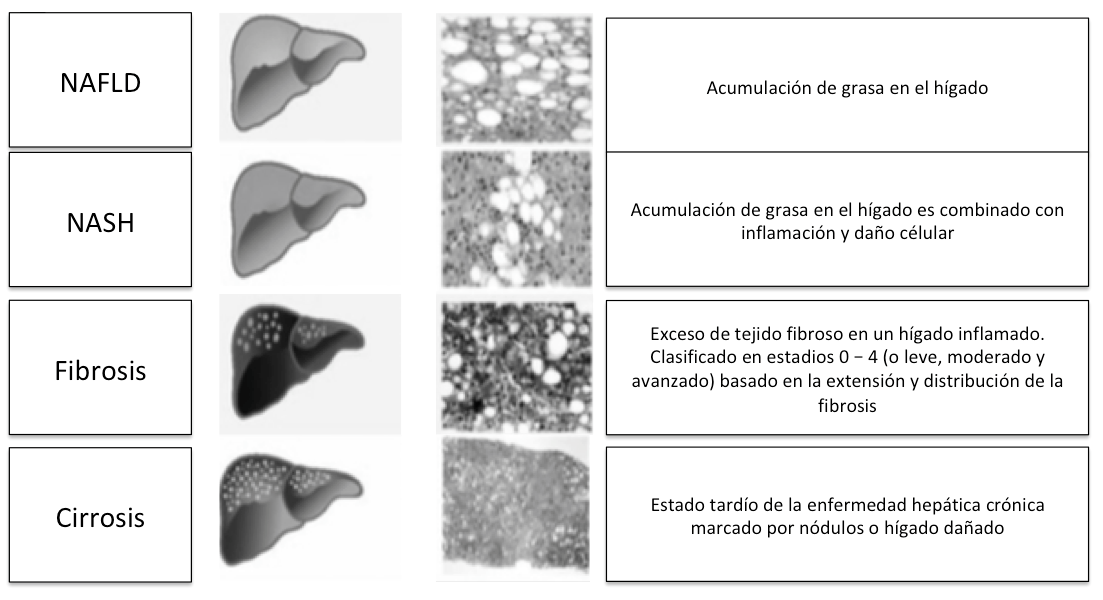
\includegraphics[height=7cm]{nafld_pato}
\caption{Estad�os de la enfermedad hep�tica cr�nica}
\label{fig:nafldpato}
\end{figure}



\subsubsection{Diagn�stico de NAFLD}

Puede ser diagnosticado por diferentes modalidades de im�genes, incluyendo el ultrasonido abdominal, que aparentemente es el mas usado \cite{de2008fatty}. Tambi�n se puede utilizar las medidas no invasivas como la tomograf�a computada y Resonancia magnetica; aunque no son confiables en reflejar el respecto de la histolog�a del h�gado en pacientes con NAFLD \cite{imajo2016magnetic}.\par


\subsubsection{Su relaci�n con el s�ndrome metab�lico}

El s�ndrome metab�lico es considerado como uno de los principales retos de salud y esta muy asociado con el NAFLD \cite{montesi2014physical}. El s�ndrome metabolico es un grupo de anormalidades que incrementan el riesgo cardiovascular. Un estudio conducido por Marchesini y Marzocchi, concluy� en que el contenido de la grasa hep�tica es significativamente mayor en pacientes con s�ndrome metab�lico comparado con los individuos libres de enfermedad, independientemente de IMC, edad o g�nero \cite{marchesini2007metabolic}.\par

\subsubsection{Insulinoresistencia (IR) y diabetes mellitus tipo 2 como factores de riesgo asociados a NAFLD}

La incidencia de NAFLD en adultos con DM2 alcanza al rededor de 75\% de la poblaci�n general \cite{jia2015non}.  El h�gado graso puede causar da�o hep�tico e inflamaci�n por estr�s oxidativo y puede progresar a fibrosis y culminar en cirrosis \cite{basaranoglu2015carbohydrate}. La insulino resistencia y el estres oxidativo son factores centrales en la patofisiolog�a de las anormalidades metab�licas de NAFLD  \cite{tilg2017nafld}.  Esto puede ser visto en la figura \ref{fig:nafldpato2}.\par

\begin{figure}[h]
\centering
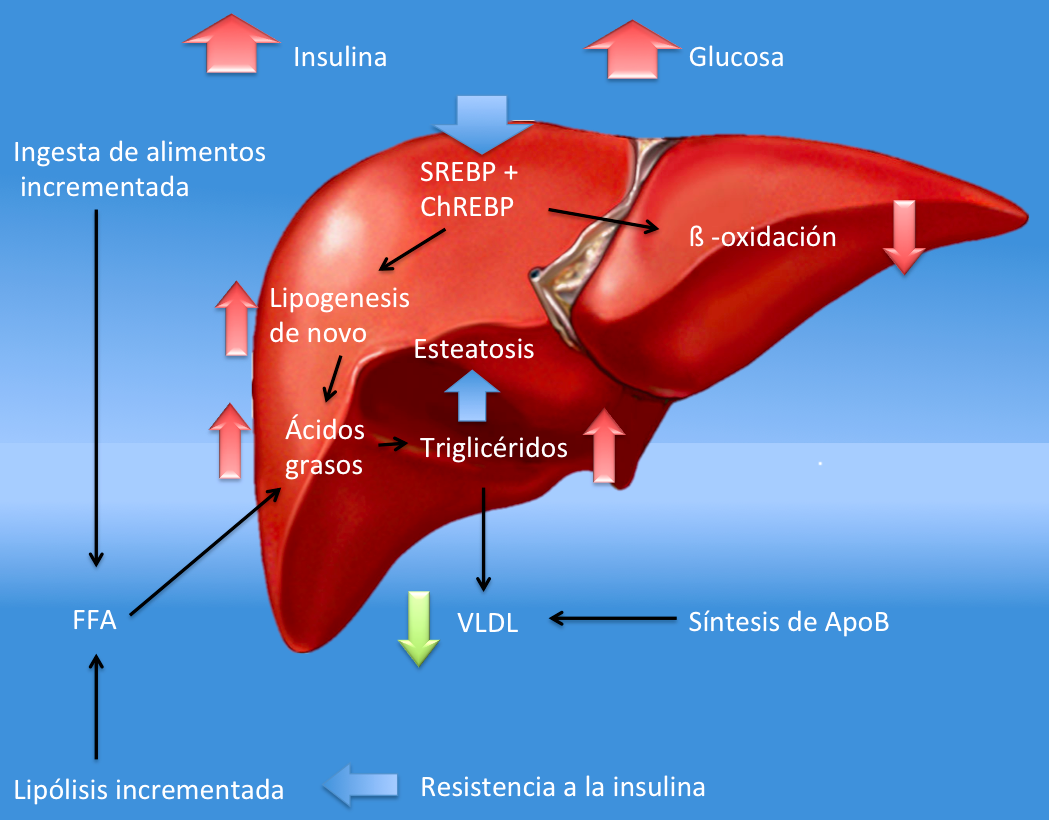
\includegraphics[height=7cm]{nafld_pato2}
\caption{Patog�nesis de la acumulaci�n de grasa dentro de las c�lulas del h�gado}
\label{fig:nafldpato2}
\end{figure}

\subsubsection{H�gado graso no alcoh�lico y Acilcarnitinas}

Recientemente Romero - Ibarguengoitia et. al. describieron un trabajo donde se relaciona el patr�n de acilcarnitinas con la presencia de obesidad e h�gado graso \cite{romero2018family} . Este estudio fue analizado mediante ecuaciones estructurales. Parte de los datos trabajados en esta tesina, corresponden a observaciones publicadas en ese art�culo. Aunque la visi�n hecha en el art�culo original, remarca la historia familiar de los pacientes y su relaci�n con obesidad. Los autores concluyen que si existe una alteraci�n en el patr�n de acilcarnitinas e inflamaci�n en los pacientes con h�gado graso. El patr�n de acilcarnitinas descrito como anormal fue el incremento de las acilcarnitinas de cadena larga (sospechando una obstrucci�n en la v�a de la beta oxidaci�n.

Por otro lado, uno de los estudios m�s representativos fue el de Statish C Kalhan y colaboradores que
incluy� 11 pacientes no diab�ticos con esteatosis hep�tica y 24 pacientes con esteatohepatitis que fueron comparados con 25 controles sanos. El patr�n metabol�mico no pudo diferenciar entre esteatosis hep�tica y esteatohepatitis; sin embargo en comparaci�n con los controles sanos las concentraciones de carnitinas libres, butirilcarnitina y metilbutiril carnitina (C3-C5) estuvo m�s alta (73). Otro estudio ha reportado tanto acilcarnitinas de cadena larga (C18, C18:2, C16) como corta (C4 yC3) relacionado a diferentes grados de
EHNA en humanos \cite{lake2015branched}.  

\subsection{Diabetes mellitus tipo 2}

La diabetes mellitus tipo 2 es una de un conjunto de enfermedades englobadas en el termino diabetes mellitus. En este y otro tipo de diabetes, varios factores gen�ticos y ambientales pueden resultar en una perdida o disfunci�n progresiva  de las c�lulas productoras de insulina (c�lulas beta), manifestandose cl�nicamente como hiperglucemia. Una vez que la hiperglucemia aparece, el paciente desarrolla un incremento a presentar complicaciones cr�nicas \cite{skyler2017differentiation} \par

La diabetes puede ser diagnosticada basandose en el criterio de glucosa plasm�tica en ayuno (FPG, por sus siglas en �ngles), a las 2 horas despu�s de una carga de tolerancia oral de glucosa (2-h PG, 2 hrs post glucose, CTOG) o con la hemoglobina glucosilada (A1c) \cite{American-Diabetes-Association:2018aa}. \par

\begin{tcolorbox}[ title = \centering Criterios para el diagnostico de Diabetes Mellitus, title filled]
\begin{itemize}
\item FPG $\geq$ 125 mg/dl (7.0 mmol/L). El ayuno definido como no ingesta calorica por al menos 8 horas*.
\item 2-h PG $\geq$ 200mg/dl (11.1 mmol/L) durante la CTOG. La prueba debe ser realizada como fue descrita por la OMS, usando una carga de glucosa que contenga 75 grs o de glucosa anh�drida disuelta en agua. 
\item A1c $\geq$ (48 mmol/mol). La prueba deber� ser realizada en un laboratorio usando el m�todo estandarizado a la prueba del DCCT.
\end{itemize}
\end{tcolorbox}

El n�mero de personas con diabetes se ha incrementado de 108 millones en 1980 a 422 millones en el 2014. La prevalencia mundial de diabetes entre adultos mayores de 18 a�os se ha incrementado de 4.7\% en 1980 a 8.5\% en 2014 \cite{mathers2006projections}. En M�xico la \textbf{E}ncuesta \textbf{N}acional de \textbf{Sa}lud y \textbf{Nut}rici�n de \textbf{M}edio \textbf{C}amino (ENSANUT MC) 2016 mostr� un ligero incremento en la prevalencia de diabetes por diagn�stico m�dico previo (9.2\%) con respecto a la encuesta del 2012 (9.2\%). El mayor incremento se observo entre los hombres de 60 a 69 a�os de edad y entre las mujeres con 60 o m�s a�os de edad, aproximadamente un 30\% de esta poblaci�n tiene diabetes \cite{hernandez2016encuesta}.


\subsubsection{La diabetes mellitus tipo2 y las acilcarnitinas}

La diabetes mellitus tipo 2 es la forma predominante de Diabetes en todo el mundo, siendo el 90\% de todos los casos \cite{melmed2016williams}. La palabra diabetes viene del griego (d�a= a trav�s de=, bainein= ir, tes=gente), es decir: ?lo que va a trav�s?, esto referido por el exceso de orina. Mellitus (del girego melli= miel) que sabe dulce o a miel (caracter�stica de la orina de estos pacientes).

El  n�mero de pacientes con diabetes esperados para el 2025 son de 300 millones de personas.  Por lo que la Diabetes mellitus tipo 2 se ha convertido en uno de los problemas mundiales de salud p�blica. En M�xico la prevalencia de la Diabetes mellitus tipo 2 es del 14.42\% (7.3 millones de personas) (3). Esta prevalencia a aumentado un 7\% comparando los resultados de la Encuesta Nacional de Salud 2006 y la Encuesta Nacional de Enfermedades Cr�nicas 2004 \cite{Villalpando:2010aa} demostrando que M�xico no es la excepci�n en el problema mundial de la Diabetes mellitus.

Este incremento tan pronunciado en la prevalencia de la Diabetes Mellitus tipo 2 es debido en parte al incremento en la prevalencia de la obesidad que en M�xico con una prevalencia combinada de sobrepeso y obesidad en mujeres mayores a 20 a�os de un 71.9\% y en hombres del 66.7\% \cite{shamah2008health}.

\begin{figure}[h]
\centering
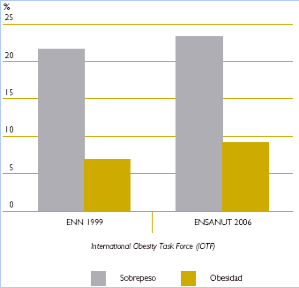
\includegraphics[width=10cm]{prev_sobre.png}
\caption{Comparaci�n de la prevalencia de sobrepeso y obesidad entre 1999 y 2006 en mujeres de 12 a 19 a�os de edad de acuerdo con los criterios propuestos por el IOTF. M�xico}
\end{figure}


\subsubsection{Fisiopatolog�a de la Diabetes Mellitus tipo 2}

La patog�nesis de la Diabetes Mellitus tipo 2 es compleja e incluyen factores gen�ticos y ambientales. Algunos de los genes descritos como predisponentes a Diabetes Mellitus tipo 2 son HHEX, SLC30A8, CDKAL1 y especialmente TCF7L2 el cual es asociado fuertemente a la enfermedad \cite{rung2009genetic}. Existen otras alteraciones gen�ticas puntuales causantes de diabetes pero son descritas como diabetes monog�nicas y sus fisiopatolog�as son distintas.
En la �ltima d�cada Ralph Defronzo describo las m�ltiples alteraciones metab�licas encontradas en el metabolismo de los carbohidratos (El ominoso octeto), en donde se describe la resistencia a la insulina. La resistencia a la insulina es una de las alteraciones precl�nicas de la diabetes mellitus y se define como la disminuci�n del efecto de la insulina en los tejidos perif�ricos.\par

\subsubsection{Teor�as de la resistencia a la insulina}
La resistencia a la insulina se manifiesta por una disminuci�n del transporte de la glucosa estimulado por la insulina, por una alteraci�n del metabolismo de la glucosa en los adipocitos y en el m�sculo esquel�tico, y por una supresi�n alterada de la producci�n hep�tica de glucosa.
La sensibilidad a la insulina est� influida por varios factores entre los que se encuentran la edad, el peso, el grupo �tnico, la grasa corporal (especialmente la abdominal), la actividad f�sica y los f�rmacos. La resistencia a la insulina se asocia con la progresi�n de la ATG y de la Diabetes mellitus tipo 2, aunque rara vez se observa una diabetes mellitus en las personas con resistencia a la insulina incluso cuando no son obesos, lo que implica la existencia de un importante componente gen�tico en el desarrollo de la resistencia a la insulina.\par

\begin{figure}[h]
\centering
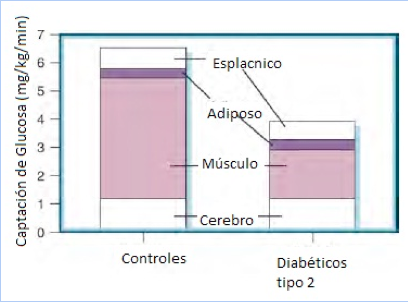
\includegraphics[width=10cm]{captacion.png}
\caption{Captaci�n de glucosa dependiente de insulina.}
\end{figure}


El principal lugar de almacenamiento de la glucosa despu�s de una comida es el m�sculo esquel�tico, y el principal mecanismo de almacenamiento de glucosa es a trav�s de su conversi�n a gluc�geno. Los estudios que utilizan la t�cnica del clamp hiperinsulinemico eugluc�mico han demostrado que en las personas resistentes a insulina con o sin DM2 hay un d�ficit en la captaci�n no oxidativa de la glucosa, en relaci�n principalmente con un defecto en la s�ntesis de gluc�geno.\par

\subsubsection{Triglic�ridos intramusculares.}

La captaci�n de glucosa estimulada por la insulina es inversamente proporcional a la cantidad de triglic�ridos intramusculares. Se ha demostrado una importante correlaci�n entre la concentraci�n de triglic�ridos intramusculares mediante biopsia, TC y resonancia magn�tica. Los familiares de primer grado de las personas con DM2 tienen un aumento de la grasa intramiocelular, y en este grupo existe tambi�n una correlaci�n con la resistencia a la insulina.\par
Esta acumulaci�n de triglic�ridos intracelulares disminuye la se�alizaci�n intracelular del receptor de insulina al mantener una fosforilzaci�n parcial del sustrato  del receptor de insulina, evitando la se�alizaci�n normal por la v�a de la MAP cinasa y terminando en la expresi�n g�nica celular; disminuye la expresi�n de canales GLUT 4 en la membrana celular y la captaci�n de glucosa por la c�lula.\par

\begin{figure}[h]
\centering
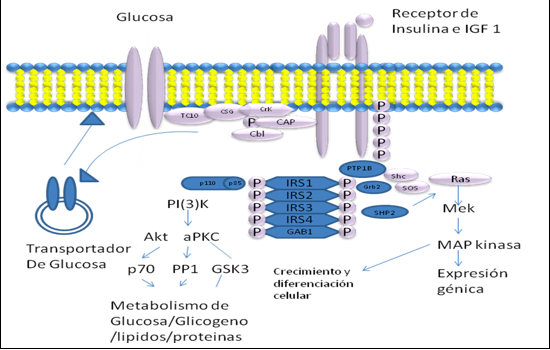
\includegraphics[width=10cm]{receptor.png}
\caption{Se�alizaci�n post receptor de insulina}
\end{figure}

\subsubsection{Fisiolog�a normal de las acil carnitinas}
En el cuerpo, los �cidos grasos son degradados a acetil-CoA la cual entra al ciclo del acido c�trico. Esta degradaci�n ocurre en la mitocondria por la beta oxidaci�n. La oxidaci�n de los �cidos grasos empieza con la activaci�n del acido graso, la reacci�n ocurre fuera y dentro de la mitocondria. \par

\begin{figure}[h]
\centering
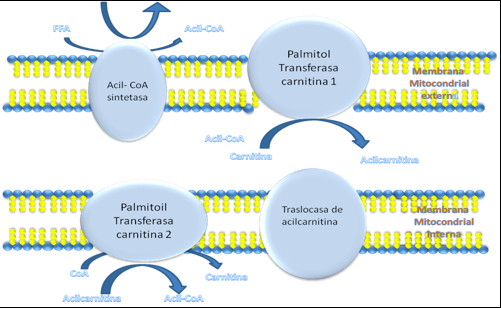
\includegraphics[width=10cm]{interna.png}
\caption{Internalizaci�n de  �cidos grasos de cadena larga a la matriz mitocondrial}
\end{figure}

Los �cidos grasos de cadena mediana y corta pueden entrar a la mitocondria sin dificultar pero los �cidos grasos de cadena larga deben entrar unidos a la carnitina con una uni�n ester antes de que pueda entrar a trav�s de la membrana mitocondrial. 
La carnitina es un b hidroxi gama trimetilamonio butirato, y es sintetizado en el cuerpo de lisina y metionina. La translocasa moviliza el ester �cido graso- carnitina dentro del espacio de la matriz en intercambio con carnitina libre. 
En el espacio de la matriz, el ester es hidrolizado haciendo el acido graso activado una mol�cula disponible para la beta oxidaci�n y proveyendo creatina libre para intercambios posteriores.  \par

\begin{figure}[h]
\centering
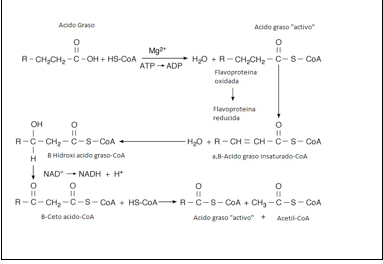
\includegraphics[width=10cm]{beta.png}
\caption{Ejemplo de la Beta oxidaci�n de un acido graso libre.}
\end{figure}

La beta oxidaci�n procede por la extracci�n de fragmentos de 2 carbonos del acido graso. La energ�a generada en este proceso es muy alta. Por ejemplo, el catabolismo de 1 mol de un acido graso de 6 carbonos que pasa a trav�s del ciclo del acido c�trico da Co2 y H2O y genera 44 mol de ATP, comparado con los 38 mol generados por el catabolismo de 1 mol de 6 carbonos de la glucosa.\par

Esta v�a de oxidaci�n de los �cidos grasos libres se mantiene inactiva mientras la c�lula es expuesta a glucosa y se activa en momentos de disminuci�n de glucosa y a la exposici�n de �cidos grasos libres.\par

\subsubsection{Evidencia de las alteraciones del metabolismo de las acilcarnitinas como etiolog�a de resistencia a la insulina.}

Recientemente se ha demostrado que la alteraci�n en la beta oxidaci�n mitocondrial es parte de la fisiopatolog�a de la resistencia a la insulina, esto al presentar diferentes patrones de acilcarnitinas s�ricas, a continuaci�n describir� algunas de las evidencias recientes.\par

Sean H. Adams et al. Encontr� en su estudio al comparar 44 mujeres obesas con diabetes mellitus tipo 2 y  12 mujeres sin diabetes mellitus (todas africano americanas), que la relaci�n de acilcarnitinas totales: carnitinas libres fue significativamente incrementada (150 a 170\%) en las mujeres con Diabetes mellitus tipo 2; adem�s la concentraci�n de �cidos grasos de cadena larga se mantuvo incrementada hasta en un 300\% en las pacientes con DM2 (p=0.004). Estos resultados son consistentes con la hip�tesis de que una beta oxidaci�n insuficiente debida en parte a la baja capacidad del ciclo del acido tricarbox�lico, incrementa la acumulaci�n de acetil CoA y genera mol�culas de acil carnitina de cadena corta que activan las v�as pro inflamatorias implicadas en la resistencia a la insulina \cite{Adams:2009aa}. \par

Kitt Falk Petersen et al. en su art�culo en el New England Journal of Medicine describe la alteraci�n mitocondrial al realizar un pinzamiento hiperinsulinemico eugluc�mico en combinaci�n de glucosa marcada en pacientes sanos, j�venes, delgados e insulinoresistentes en desendientes de pacientes con diabetes mellitus tipo 2, comparados con sujetos controles insulinosensibles pareados por edad, peso y actividad f�sica. Realizaron una resonancia magn�tica con espectroscopia para medir el contenido lip�dico intramiocelular e intra hep�tico adem�s de la evaluaci�n de la raz�n de la actividad de fosforilaci�n oxidativa mitocondrial en el m�sculo. Encontraron que la raz�n de captura de glucosa estimulada por insulina en el m�sculo fue aproximadamente 60\% m�s baja en los sujetos insulinoresistentes que en los sensibles a la insulina (p=<0.001) y fue asociado a un incremento del 80\% en el contenido lip�dico intramiocelular (p=<0.005) \cite{Mohlig:2004aa}.\par

M. M�der � A. Kie�ling et al. Demostraron que los pacientes con Diabetes mellitus tipo 2 presentan una alteraci�n en el patr�n urinario de las acilcarnitinas que concuerda con los cambios a nivel s�rico. \par

\begin{figure}[h]
\centering
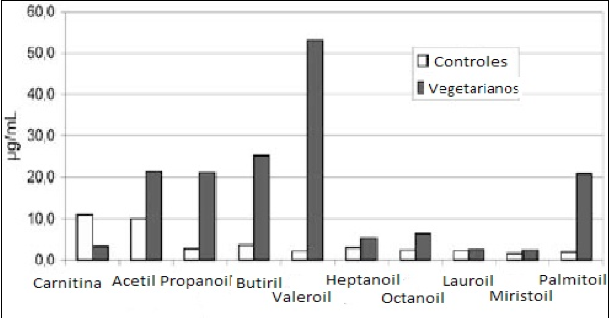
\includegraphics[width=10cm]{acilcarni.png}
\caption{Acil carnitinas urinarias en sujetos controles}
\end{figure}

Estos pacientes ten�an mayor concentraci�n urinaria de acilcarnitinas de cadena larga (principalmente palmitoil carnitina) mediante el an�lisis de inyecci�n de flujo- electroscopia de masas inonizaci�n electro espray.\par


\begin{figure}[h]
\centering
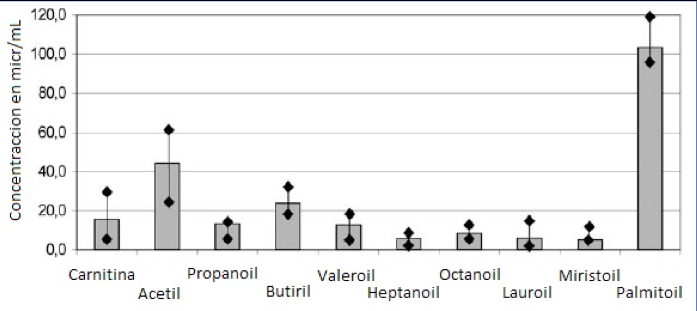
\includegraphics[width=10cm]{uri.png}
\caption{Concentraciones urinarias de acilcarnitinas en personas con DM2.}
\end{figure}


\subsection{Retinopat�a}
El t�rmino retinopat�a se refiere a la presencia de alg�n da�o no especificado en la membrana sensible a la luz del ojo llamada retina. Una de las principales causa de retinopat�a es la diab�tica, la cual es la principal causa de ceguera en los Estados Unidos, fue inicialmente descrita por Eduard Jaeger en 1856, pero sus relaciones causales entre los ex�menes de retina y la diabetes mellitus fueron inicialmente controversiales hasta 1875 cuando Leber confirmo los hallazgos \cite{Wolfensberger:2001aa}.\par

En el 2005, 5.5 millones de personas ten�an retinopat�a diab�tica y 1.2 millones se encontraban en peligro de padecerla \cite{Shah:2017aa}. En M�xico existe un estudio que evalu� la prevalencia de retinopat�a diab�tica encontrandose que mas del 34\% de la poblaci�n estudiada tenia retinopat�a no proliferativa \cite{Gonzalez-Villalpando:1994aa}.\par
Existen dos categor�as principales de retinopat�a diab�tica: no proliferativa y prolifrativa. El edema macular diab�tico puede presentarse en cualquier etapa. La diferenciaci�n entre ambas etapas de la retinopat�a es la proliferaci�n de nuevos vasos sangu�neos los cuales son altamente predisponentes a presentar sangrados y exudados de materiales lip�dicos \cite{gardner2007greenspan}.

\subsubsection{Revisi�n de fondo de ojo y el lecho vascular sist�mico}

La forma no invasiva de conocer el estado de la vasculatura sist�mica es a trav�s de la visualizaci�n de los vasos retinianos (mediante la lampara de hendidura), que provee un campo de estudio de c�mo diversas patolog�as cambian la microcirculaci�n humana.  La tecnolog�a actual permite hacer una medici�n objetiva de dichos cambios. Los vasos retinianos no tienen inervaci�n adren�rgica que pueda iniciar cambios en el tono vascular \cite{ye1990peptidergic},\cite{laties1967central}, se ha postulado que el di�metro vascular es dependiente de cambios miog�nicos \cite{dumskyj1996autoregulation}, as� como v�as que involucran la funci�n endotelial, inflamaci�n y autorregulaci�n metab�lica a trav�s de elaboraci�n de factores vasodilatadores (�xido n�trico, adenosina, prostanoides) y vasocontrictores (endotelina, angiotensina II) en respuesta a demandas metab�licas. El �xido n�trico juega un papel central en la regulaci�n del tono vascular e inhibie la adhesi�n plaquetaria y leucocitaria en las c�lulas endoteliales \cite{roufail1995nitric}, \cite{nagaoka2002effect},\cite{vecchione2002leptin}. Otros marcadores de inflamaci�n como el complemento y las interleucinas, niveles elevados de prote�na C, interleucina 1, 6 y TNF alfa se asocian a mayor di�metro venular independiente de la presi�n arterial y diabetes Mellitus (24). Recientemente se ha demostrado que la PCR puede tener efectos sobre la vasorreactividad del �xido n�trico en el endotelio retiniano arteriolar (25). La IL 10 se asocia a mejor reactividad del sistema vascular y suele encontrarse disminuida en pacientes con obesidad y los niveles de IL 17 se asocian a la mayor estimulaci�n de citocinas IL- 6 y 8. \par

En base a lo descrito previamente se realiz� el estudio de Romero - Ibarguengoitia \cite{Romero-Ibarguengoitia:2017aa}, donde se documenta la relaci�n de lesiones retinianas en pacientes con obesidad y sin diabetes. En este trabajo se continua con la intenci�n de poder clasificar estos pacientes como portadores de lesiones retinianes con las acilcarnitinas, que como se mencion� en la secci�n de NAFLD, tienen relaci�n con inflamaci�n y la presencia de obesidad.





\section{Estudios Estad�sticos previos}

Han existido m�ltiples intentos de realizar un diagnostico certero del h�gado graso no alcoh�lico mediante pruebas bioqu�micas. En el presente trabajo se hace menci�n de cuatro estudios previos basados en algoritmos de aprendizaje maquina \cite{Oh:2016aa}. Se separar� la informaci�n de la literatura en sub secciones correspondientes a las diferentes complicaciones del s�ndrome metab�lico.\par


\subsection{H�gado graso no alcoh�lico.}

\subsubsection{SteatoTest}

En el 2005 el grupo de trabajo de Thierry Poynard et. al. (2005) publicaron un estudio donde validan una herramienta para la predicci�n de h�gado graso \cite{Poynard:2005aa}.  En su publicaci�n remarcan la importancia y riesgo de realizar una biopsia de h�gado graso durante la evaluaci�n de la enfermedad hep�tica cr�nica.\par

Para el an�lisis de este estudio se incluyeron 2,272 sujetos, siendo 884 sujetos incluidos para la validaci�n del biomarcador.  El SteatoTest surge de un modelo de regresi�n log�stica y las 12 variables predictoras contenidas en el modelo son: Transaminasa Glut�mico Piruvica (TGP), $\alpha_2$-microglobulina (A2M), apolipoprote�na A-1 (ApoA1), haptoglobina, bilirrubina total, Gama glutamil transpeptidasa, colesterol, triglic�ridos, glucosa, edad, g�nero e �ndice de masa corporal.  La divisi�n de los pacientes se pueden ver en la figura \ref{fig:steatotest}  .\par

\begin{figure}[h]
\centering
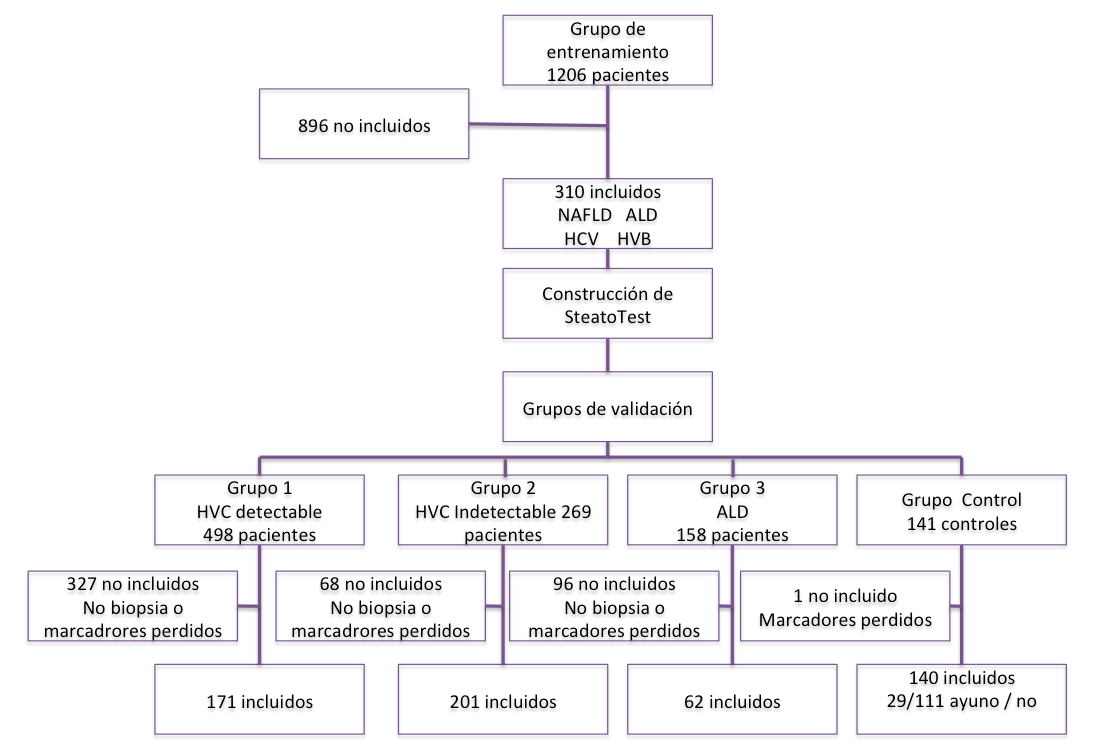
\includegraphics[width=13cm]{steatotest}
\caption[Distribuci�n de pacientes en la validaci�n de SteatoTest]{pie}
\label{fig:steatotest}
\end{figure}

En la tabla \ref{tab:auc_steto}, se puede observar como el SteatoTest tiene una mayor �rea bajo la curva ROC, en comparaci�n con biomarcadores cl�sicamente relacionados a la presencia de esteatohepatitis.  Los autores concluyen que el SteatoTest es un estimador simple y no invasivo que estima la esteatosis hep�tica y puede reducir la necesidad de biopsia hep�tica, particularmente en pacientes con factores de riesgo metab�lico.\par


\begin{table}
\begin{tabular}{cccccc}\hline
\begin{minipage}[t]{0.15\textwidth}\centering \textbf{Panel} \\ \textbf{Diagn�stico}\end{minipage} & \begin{minipage}[t]{0.15\textwidth} \centering \textbf{Grupo de} \\\textbf{entrenamiento} \end{minipage} & \textbf{Grupo 1} & \textbf{Grupo 2} & \textbf{Grupo 3} & \begin{minipage}[t]{0.15\textwidth} \centering \textbf{  Todos} \\ \textbf{los grupos}\end{minipage}  \\
&&&&&\\
 & N= 310 & N = 171 & N = 201 & N = 62 & N = 884\\
SteatoTest & 0.79 (0.03)* & 0.80 (0.04)\textsterling & 0.86 (0.03)\$ & 0.72 (0.05)** & 0.8 (0.02)\textsterling\textsterling\\
GGT & 0.66 (0.03) & 0.67 (0.05) & 0.74 (0.05) & 0.50 (0.09) & 0.66 (0.02)\\
ALT & 0.58 (0.03) & 0.62 (0.05) & 0.79 (0.04) & 0.66 (0.07) & 0.61 (0.02)\\

\multicolumn{6}{l}{
\begin{minipage}[t]{1\textwidth}
\vspace{0.1cm}
\footnotesize{* Mayor que GGT (p<0.0001 y ALT (p<0.0001); \textsterling Mayor que GGT (p=0.007) y ALT (p<0.0001);
\\ \footnotesize{\$ Mayores que GGT(p= 0.02); ** Mayor de GGT (p= 0.002); \textsterling \textsterling Mayor que GGT (p <0.0001) y ALT (p<0.0001)} }
\end{minipage}
}
\end{tabular}
\caption{�reas bajo la curva ROC de SteatoTest, GGT, ALT para el diagnostico de esteatosis mayor al 5\% en grupos de entrenamiento y validaci�n.}
\label{tab:auc_steto}
\end{table}

\subsubsection{NASH Test.}

En el 2006 Thierry Poynard et. al. publicaron el valor diagn�stico de marcadores bioqu�micos (Nash Test) con la intenci�n de predecir la presencia de esteatohepatitis no alcoh�lica  en pacientes con h�gado graso no alcoh�lico \cite{Poynard:2006aa}.  Este grupo de trabajo ha desarrollado multiples herramientas de marcadores bioqu�micos para la detecci�n de fibrosis hep�tica (FibroTest) y de h�gado graso (SteatoTest, ya presentado anteriormente).\par

La poblaci�n estudiada para la validaci�n del Nash Test consiste en la misma para el FibroTest, con criterios de inclusiones son iguales para ambos grupos de validaci�n, la �nica diferencia en el presente estudio fue la exclusi�n de pacientes sin esteatosis histol�gica. Adem�s se excluyeron los sujetos que ten�an un consumo de alcohol mayor a 50 grs por d�a para el hombre o 30 grs para las mujeres durante el a�o anterior al estudio; ademas de tener panel viral negativo y VIH negativo. Enfermedades gen�ticas como al enfermedad de Wilson o deficiencia de alfa 1 antitripsina. El modelo utilizado para el an�lisis fue un modelo de regresi�n log�stica con pesos espec�ficos (no mostrados).\par

Los par�metros cl�nicos que mas discriminan son el peso y el g�nero, AST, GGT y glucosa para los par�metros biol�gicos. En la figura \ref{fig:nashtest}  se puede observar la curva ROC para el NashTest, donde no hay diferencia entre las curvas ROC entre los datos de entrenamiento y de validaci�n p = 0.34. Los autores concluyen que deben ser seleccionados los pacientes a los que se les indica realizar esta prueba.

\begin{figure}[h]
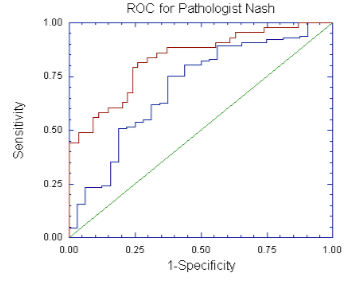
\includegraphics[width=12cm]{nashtest}
\caption{Curva ROC de NASHTest para el diagnostico de NASH por el pat�logo en los grupos de entrenamiento y validaci�n}
\begin{minipage}[t]{1\textwidth} \centering \footnotesize{La linea roja corresponde al grupo de entrenamiento y la l�nea azul la de validaci�n} \end{minipage}
\label{fig:nashtest}
\end{figure}

\subsubsection{NASH Diagnostics}

Younossi et. al. describieron en el 2008 un panel para diagnosticar la esteatohepatitis no alcoh�lica asociada a obesidad \cite{Younossi:2008aa}.  El estudio incluy� 101 pacientes con biopsias hep�ticas quienes fueron evaluados mediante pruebas ELISA, para diferentes mol�culas. De estos, 69 fueron incluidos en los datos de entrenamiento y 32 en los datos de validaci�n. Los datos cl�nicos fueron obtenidos al mismo tiempo de la biopsia hep�tica. Las muestras fueron recolectadas en ayuno, los biomarcadores inclu�dos fueron la adiponectina, resistina, insulina, glucosa, TNF-alfa, IL-6, IL-8, citoqueratina, CK-18 y M30.\par
\newpage
\begin{figure}
\centering
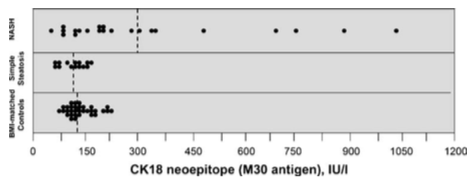
\includegraphics[width=12cm]{nashdiag}
\caption{Niveles del neoepitope CK-18 est�n significativamente incrementados en el suero de pacientes con NASH}
\label{fig:nashdiag}
\end{figure}


En la figura \ref{fig:nashdiag}, se observa la distribuci�n del epitope Ck-18, en este estudio se decidi� utilizar un modelo lineal m�ltiple para predecir NASH, tabla (\ref{tab:modelonash}). \\~\\


\begin{table}[h]
\centering
\begin{tabular}{ccccc}\hline
Modelo & \begin{minipage}[t]{0.14\textwidth} \centering Variable\\ Independiente \end{minipage} & Betas y SE & \begin{minipage}[t]{0.14\textwidth}\centering p values variables \\independientes\end{minipage} & \begin{minipage}[t]{0.14\textwidth}\centering p todo \\ el modelo \end{minipage}\\\hline
\begin{minipage}[t]{0.14\textwidth}\centering Predicci�n de NASH \end{minipage} & (Intercepto) & 0.4909 $\pm$ 0.1351 & <0.0006 & p<1.232e\textsuperscript{-6}\\
& M30, IU/L & 0.0011 $\pm$ 0.0003 & <0.0001 &\\
& M65-M30, IU/L &  0.0003 $\pm$ 0.0001 & <0.0548 & \\
&Adiponectin, $\mu$g/ml & -0.0153 $\pm$0.0069 & <0.0316 & \\
&Resistin, ng/ml & -0.0418 $\pm$ 0.0125 & <0.0014\\
\hline
\multicolumn{5}{l}{ \footnotesize{SE = error est�ndar del estimado}}
\end{tabular}
\caption{Modelo de regresi�n lineal multiple para la predicci�n de NASH}
\label{tab:modelonash}
\end{table}

El modelo lineal a mi parecer no es el modelo mas adecuado ya que aunque se ordenaron los posibles valores de la variable NASH, seria mejor utilizar un modelo multinomial o regresi�n log�stica, ya que los datos con categ�ricos ordenados. El desempe�o del modelo en los datos de validaci�n fue caracterizado por un AUC de 0.732 (95\% IC, 0.55 - 0.87). Con un limite del modelo de 0.325, fue asociado con una sensibilidad de 71.4\%, especificidad de 72.7\%, valor predictivo positivo de 83.3\%, y un valor predictivo negativo de 57.1\%.  Los autores concluyen que esta herramienta de unir a cuatro estudios basados en ELISA es adecuado para formar un biomarcador diagn�stico simple para NASH.

\subsubsection{Modelo NICE}

El \textbf{N}on -\textbf{i}nvasive \textbf{c}omposite \textbf{m}odel (Nice model) fue descrito por Anty et. al.  en el 2010 \cite{anty2010new}, esto con el objetivo de desarrollar un sistema de medici�n para el diagn�stico definitivo de NASH usando datos cl�nicos y biol�gicos relacionados a el s�ndrome metab�lico y el da�o hep�tico incluyendo el fragmento CK 18 generado por la caspasa 3.\par

Se incluyeron 464 obesos morbidos, referidos para cirug�a bari�trica, los paciente fueron enrolados entre el 2003 y 20009. Los pacientes fueron arbitrariamente divididos en dos grupos 1) datos de entrenamiento de 310 pacientes (43 hombres, 267 mujeres), y 2) grupo de validaci�n consistente de 154 pacientes. Se excluyeron pacientes con marcadores de hepatitis B y C , y la presencia de consumo de alcohol mayor a 24 grs/d�a. El modelo utilizado fue una regresi�n log�stica.\par

\begin{table}[h]
\centering
\begin{tabular}{|c|c|c|c|}\hline
& P-value & OR & 95\% IC\\\hline
ALT & 0.002 & 1.04 & 1.01 - 1.07\\\hline
GGT & 0.6 & 0.99 & 0.98 - 1.01  \\\hline
HOMA - IR & 0.6 & 0.98 & 0.92 - 1.05 \\\hline
CK18 & 0.044 & 1.003 & 1.00006 - 1.005\\\hline
Genero & 0.7 &0.82 & 0.21 - 3.19 \\\hline
IDF MS & 0.005 & 7.3 & 1.8 - 29.4 \\\hline
\multicolumn{4}{l}{ \footnotesize{
\begin{minipage}[t]{0.6\textwidth}
ALT = alanino amino transferasa, GGT, gama glutamil transpeptidasa, HOMA-IR, homeostasis model assessment of insulin resistance,IDF MS, s�ndrome metab�lico seg�n la federaci�n internacional de diabetes\end{minipage}}}
\end{tabular}
\caption{An�lisis multivariado de los datos de entrenamiento}
\label{tab:log_nice}
\end{table}

Como se aprecia en la tabla \ref{tab:log_nice}, se mantienen dentro del modelo tres variables que aparentemente no aportan significancia (GGT, HOMA-IR, Genero) al modelo.  En el figura \ref{fig:roc_nice} , se puede observar la eficacia seg�n el �rea bajo la curva ROC, que aunque no se realiz� una prueba para determinar diferencia entre ellas, no tienden a ser diferentes la curva de los datos de entrenamiento y los de validaci�n.\par


\begin{figure}[h]
\centering
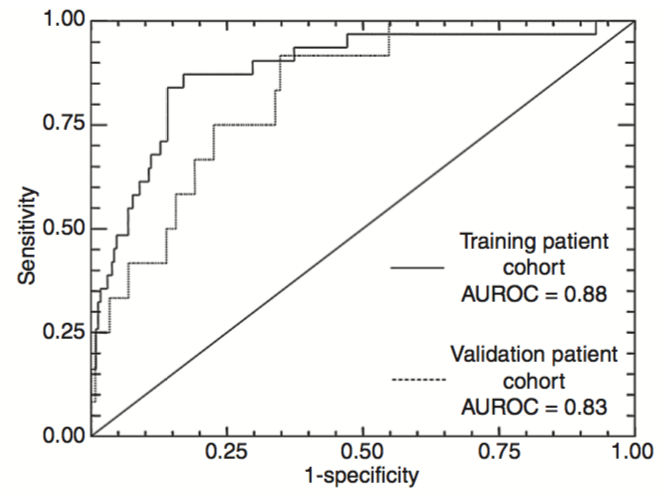
\includegraphics[width=8cm]{roc_nice}
\caption{Curvas ROC del modelo en datos de entrenamiento y validaci�n}
\label{fig:roc_nice}
\end{figure}

Los autores concluyen que el Nice model puede ser usado con el s�ndrome metab�lico para predecir la presencia de NAFLD en pacientes con obesidad morbida.\par


\subsection{Diabetes mellitus}

\subsubsection{ELSA-Brasil}

Rodrigues-Olivera et. al.  publicaron en Sao Paulo Medical Journal en 2017, un estudio transversal con el objetivo de clasificar los pacientes con diabetes mellitus en base a antecedentes familiares, edad, h�bitos de buena salud, consumo de otras substancias. Las variables tomadas en cuenta se describen en la tabla \ref{tab:elsa}.\par


\begin{table}[h]
\centering
\begin{tabular}{|p{2cm}|p{2cm}|p{2cm}|p{2cm}|p{2cm}|}\hline
Consumo de sal & �ndice Cintura - cadera & Ingreso & Uso de bicicleta& G�nero \\\hline
Actividad f�sica & Consumo de alcohol & Consumo Frutas & Consumo vegetales & Diabetes mellitus \\\hline
Educaci�n & Tabaquismo & Edad & IMC & Terapia antihipertensiva \\\hline
Uso de hipolipemiantes & Falla cardiaca &  Infarto al miocardio & Revascula- rizaci�n & Stroke\\\hline
Calidad de Sue�o & Estado Civil & Dolor al caminar & Consumo de caf� & Ant. Hipertensi�n \\\hline
Ant. Diabetes & Colesterol elevado &  &&\\\hline
\end{tabular}
\caption{Caracter�sticas de ELSA-brazil}
\label{tab:elsa}
\end{table}

\newpage

En este estudio se utilizaron tambi�n multiples algoritmos para llevar acabo la clasificaci�n, y son: regresi�n log�stica, perceptron multicapa/backpropagation, n�ive Bayes classfier, k vecino mas cercano y random forest.  Al inicio se evaluaron 15,105 sujetos, que despu�s de los la exclusi�n por falta de datos se incluyeron 12,447 sujetos para el estudio de los cuales el 30\% de ellos fueron separados para incluirlos en el grupo de prueba. En la figura \ref{fig:elsa}  se muestra el proceso de la construcci�n del modelo.\par

\begin{figure}
\centering
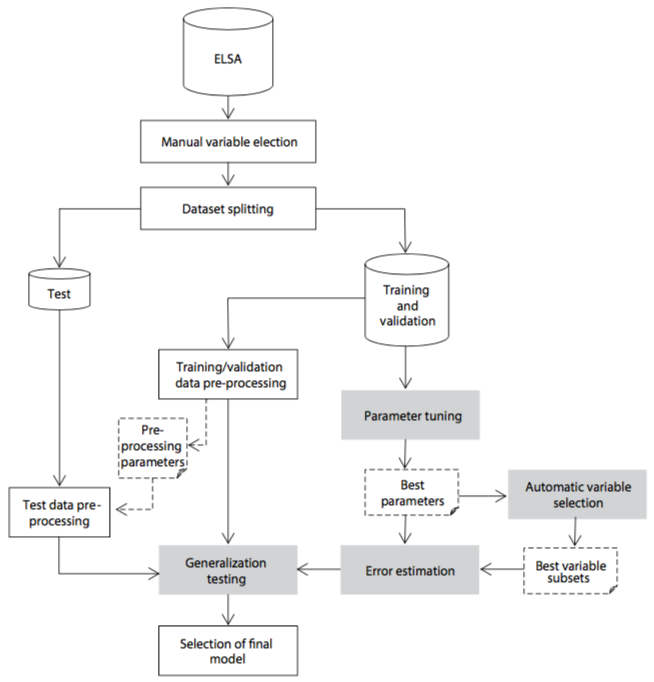
\includegraphics[height=8cm]{elsa}
\caption{Proceso general de la construcci�n del modelo y su evaluaci�n}
\label{fig:elsa}
\end{figure}

En la tabla \ref{tab:elsa_gen}  se puede observar como los alcanzaron una �rea bajo la curva (AUC) bastante pobre y no fueron mejores en sensibilidad y especificidad.\par

\begin{table}
\begin{tabular}{|c|c|c|c|c|c|c|}\hline
\multicolumn{3}{|c|}{ Estimaci�n del error} &&&\multicolumn{2}{|c|}{ Generalizaci�n}\\\hline
Algoritmo& AUC & BA & AUC & BA & Sensibilidad & Especificidad \\\hline
LR & 75.44\% & 69.30\% & 74.41\% & 67.62\% & 67.99\% & 67.24\%\\\hline
ANN & 75.45\% & 69.36\% & 74.17\% & 67.78\% & 66.25\% & 69.30\%\\\hline
NB & 74.85\% & 68.95\% & 74.06\% & 68.52\% & 74.94\% & 62.1\% \\\hline
KNN & 74.98\% & 68.52\% & 73.35\% & 67.76\% & 70.97\% & 64.55\% \\\hline
RF& 72.81\% & 67.06\% & 72.35\% & 67.5\% & 67.74 \% & 67.24\% \\\hline
\end{tabular}
\caption{Generalizaci�n de los resultados de prueba}
\label{tab:elsa_gen}
\end{table}

Los autores concluyen que todos los algoritmos tienen la misma efectividad para clasificar a los pacientes con diabetes mellitus; sin embargo, este estudio tiene la debilidad que es no contar con muchas variables biol�gicas que aporten informaci�n a los modelos.\par


\subsubsection{Identificaci�n de individuos con prediabetes y diabetes mediante �rboles de decisi�n}

Una identificaci�n m�s f�cil o temprana de paciente con prediabetes y/o diabetes es una tarea que es perseguida por muchos investigadores, Hische et. al \cite{hische2010decision} describi� en el 2010 un modelo predictivo basado en �rboles de decisi�n. El algoritmo utilizado por los autores es el descrito por Quinlan, C4.5 Las variables utilizadas para la creaci�n de este modelo incluyeron entre otras, edad, g�nero, medidas relacionadas al peso (IMC, �ndice cintura-cadera, HOMA-IR, glucosa e insulina. \par

En este estudio se utilizaron dos cohortes, una del ``cross-sectional \textbf{M}etabolic \textbf{S}yndome \textbf{B}erlin \textbf{P}otsdam \textbf{S}tudy (Mesy-Bepo) en la cual se incluyeron 1737 individuos sin diabetes (todos mayores de 18 a�os) y de la cohorte Dresden, donde se incluyeron 1998 sujetos con historia familiar de diabetes mellitus, obesidad o dislipidemia.

\begin{figure}
\centering
\begin{subfigure}[t]{0.4\textwidth}
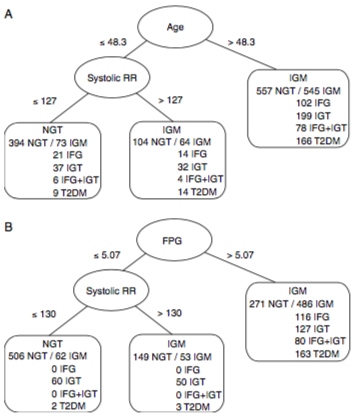
\includegraphics[height=5cm]{mesy}
\caption{�rbol de decisi�n basado en (A) cl�nica y (B) Laboratorio en la cohorte Mesy-Bepo}
\end{subfigure}
\begin{subfigure}[t]{0.4\textwidth}
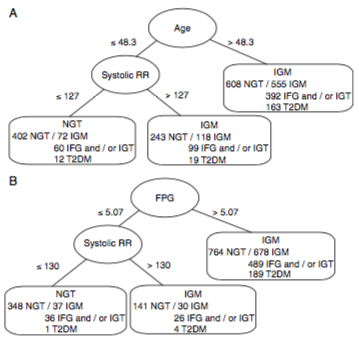
\includegraphics[height=5cm]{dresden}
\caption{�rbol de decisi�n basado en (A) cl�nica y (B) Laboratorio en la cohorte Dresden}
\end{subfigure}
\end{figure}

El desempe�o de los modelos se observa en la tabla \ref{tab:potsdam}  .

\begin{table}
\begin{tabular}{cccccc}\hline
& Datos & Sensibilidad (\%) & Especificidad (\%) & VPP (\%) & VPN (\%)\\\hline
Mesy-Bepo & C�nica & 89.3 & 37.4 & 48& 84.4 \\
 & Lab & 89.7 & 54.6 & 56.2 & 89.1 \\
Dresden& Cl�nica & 90.3 & 32.1 & 44.2 & 84.8 \\
&  lab & 95 & 27.8 & 43.9 & 90.4 \\\hline
\end{tabular}
\caption{Tabla de desempe�o de los estudios Mesy-Bepo y Dresden}
\label{tab:potsdam}
\end{table}

\subsubsection{Predicci�n de diabetes mediante �rboles de decisi�n}

Cada vez existe mas literatura m�dica en donde se utiliza el aprendizaje maquina para el an�lisis de los datos. uno de estos art�culos recientes es el de Habibi et. al. (2015) quienes trabajaron con el objetivo de producir un modelo predictivo usando caracter�sticas asociadas a diabetes mellitus tipo 2 \cite{habibi2015type}. Los datos fueron obtenidos retrospectivamente del centro de control en diabetes mellitus del Este de Azerbajian. se Incluyeron 22,398 sujetos que ten�an la categor�as de persona con diabetes, prediabetes y sano, dentro de los cuales 924 (4.1\%) ten�an diabetes, 3,062 (13.7\%) eran prediab�ticos, y 18,412 (82.2\%) eran sanos. Utilizaron el algoritmo de C4.5 descrito por Quinlan, en Weka (J48).\par

Las caracter�sticas utilizadas para la clasificaci�n incluyeron, edad, g�nero, presi�n sist�lica, diast�lica, historia familiar de diabetes, e �ndice de masa corporal. No se incluyeron variables como glucosa y triglic�ridos. La efectividad del modelos se puede ver en la tabla \ref{tab:ref_dt}  .\par

\begin{table}
\centering
\begin{tabular}{|c|c|c|c|c|c|c|}\hline
& ROC & F-Measure & Recall & Precision & Accuracy & FP rate\\\hline
results & 0.875 & 0.705 & 0.694 & 0.717 & 0.976 & 0.012\\\hline
\end{tabular}
\caption{Resultados de la evaluaci�n del modelo}
\label{tab:ref_dt}
\end{table}

El modelo obtenido se muestra en la figura \ref{fig:dt_ref1} .

\begin{figure}[h]
\centering
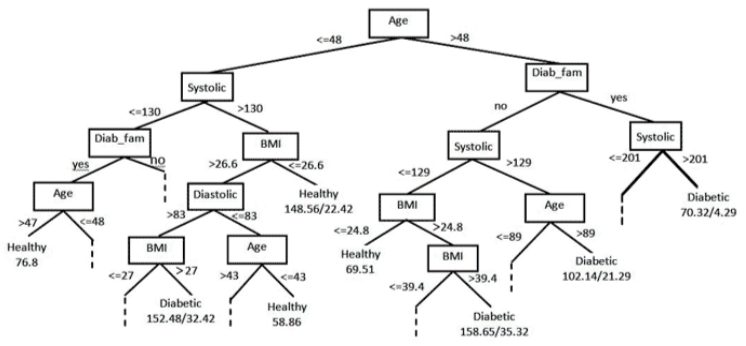
\includegraphics[height=5cm]{dt_ref1}
\caption{Modelo obtenido para la predicci�n de diabetes}
\label{fig:dt_ref1}
\end{figure}

Los autores concluyen que  aportaron a la literatura m�dica un algoritmo que pudiera ser de utilidad para el escrutinio de diabetes mellitus que no utiliza ninguna variable de laboratorio, aunque esto puede disminuir la efectividad del modelo.

\subsection{Retinopat�a}

En este cap�tulo se hablara poco sobre los modelos ya creados para clasificar la retinopat�a, ya que la mayor�a de estos modelos son para evaluaci�n de las im�genes obtenidas de la revisi�n del fondo de ojo y no de las caracter�sticas cl�nicas y/o metabol�micas. En la revisi�n de la literatura se hablar� un poco mas sobre esta relaci�n encontrada por Romero-Ibarguengoitia et. al (2018).

\subsubsection{Aplicaci�n de apoyo cl�nico, para el diagnostico de retinopat�a diab�tica.}


Esta aplicaci�n fue desarrollada por Romero-Aroca et.al, y publicada en Telemedicine and e-Health en el 2017 \cite{romero2018clinical}.  Esta aplicaci�n se desarroll� de una muestra de 2,323 pacientes divididos en 1,212 pacientes de entrenamiento y 1,111 de prueba. La aplicaci�n se baso en el algoritmo de ``fuzzy random forest''. En la figura \ref{fig:fuzzy}  se puede observar los pasos realizados para la realizaci�n del modelo.

\begin{figure}[h]
\centering
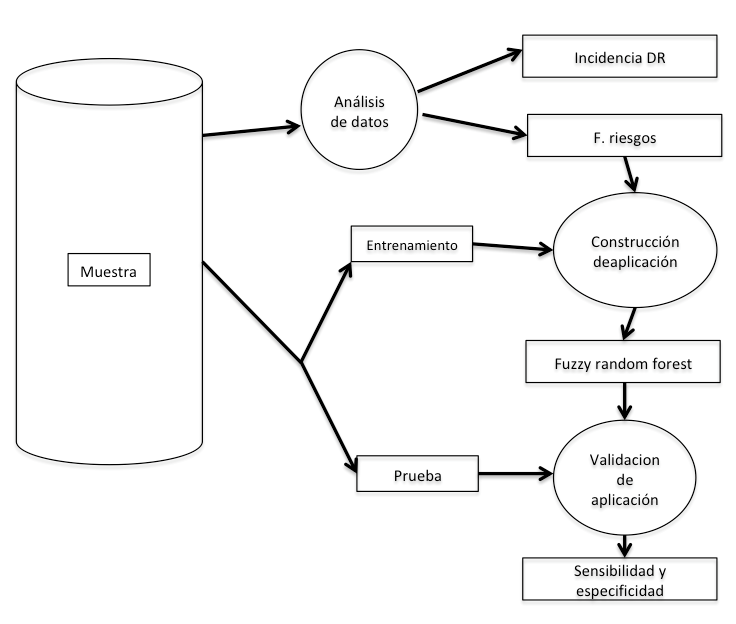
\includegraphics[height=5cm]{fuzzy}
\caption{Diagrama de flujo para la creaci�n de la aplicaci�n}
\label{fig:fuzzy}
\end{figure}

En la tabla \ref{tab:fuzzy}  se muestra la comparativa de diferentes algoritmos de predicci�n con el Fuzzy Random Forest, se documenta ser mas balanceado el �ltimo. Las variables mas importantes para clasificaci�n de la retinopat�a diab�tica es la: edad, g�nero, tratamiento con insulina, hipertensi�n arterial, A1c\%, IMC , microalbuminuria.

\begin{table}[H]
\centering
\begin{tabular}{cccccc}\hline
 & ID3 & KNN & LR & RF & Fuzzy RF\\\hline
Sensibilidad & 60\% & 25.2\% & 51.4 \% & 80\% & 80.6\%\\\hline
Especificidad & 66.7\% & 77.5\% & 94.4\% & 80.1\% & 85.9\%\\\hline
\end{tabular}
\caption{Comparaci�n de sensibilidad y especificidad, usando diferentes m�todos}
\label{tab:fuzzy}

\end{table}

El autor concluye que esta aplicaci�n puede ayudar al escrutinio de retinopat�a diab�tica, aunque es necesario mayores estudios.






\section{Antecedentes de �rboles de decisi�n en S�ndrome Metab�lico}

Dentro de la planificaci�n y del an�lisis de los datos, se realizo una primera exploraci�n de los datos en donde, se decidi� evaluar la efectividad de un �rbol de decisi�n creado por el experto (esto es, un  endocrin�logo), y que fue validado por otro endocrinologo. La forma de realizaci�n de este �rbol fue  orientado puramente en caracter�sticas cl�nicas y no se tomaron en cuenta, las caracter�sticas bioqu�micas. \par
La raz�n de este desarrollo fue identificar: 1) que las variables cl�nicas no son suficientes para la adecuada clasificaci�n de los pacientes con s�ndrome metab�lico, y 2) a�n el experto necesita de una herramienta que mejore la capacidad predictiva en la vida diaria

\begin{figure}[h]
\centering
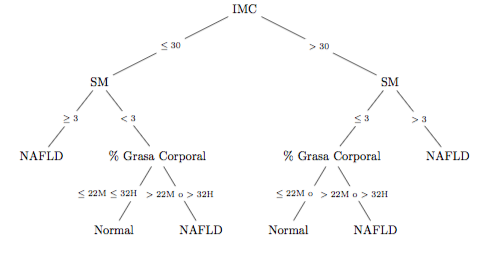
\includegraphics[height=5cm]{sm_dt}
\caption{�rbol de decisi�n creado por el experto}
\label{fig:sm_dt}
\end{figure}

En la figura \ref{fig:sm_dt} se logra ver que solo se cuentan con variables encontradas en la exploraci�n f�sica y que tambi�n pone en consideraci�n el g�nero de la persona. Todas las variables con caracter�sticas usadas por el Criterio de ATP III (Adult Treatment Panel III) para la clasificaci�n de s�ndrome metab�lico.\par

\begin{table}[h]
\centering
\begin{tabular}{|c|c|c|c|c|}\hline
Sensibilidad & Especificidad & VPP & VPN & Exactitud\\\hline
23\% & 78\% & 70\% & 31\% & 40.1\% \\\hline
\end{tabular}
\caption{Desempe�o del �rbol de decisi�n por el ATP III}
\label{tab:atp}
\end{table}

Como se observa en la tabla \ref{tab:atp}, este �rbol de decisi�n, no cuenta con suficiente exactitud para ser usado en todos los casos, aunque la especificidad del modelo es alta. El valor predictivo positivo tal vez nos permita considerarlo en ocasiones individuales.
\section{Justificaci�n y objetivos del trabajo}

La justificaci�n a este trabajo nace de la necesidad de tener herramientas que demuestren ser efectivas en solucionar los problemas en la investigaci�n m�dica y que puedan ser llevadas a la pr�ctica cl�nica diaria, ya que aunque es necesaria la investigaci�n de nuevo conocimiento y caracterizaci�n de las enfermedades, es prioritario generar mayores recursos para una correcta toma de decisiones.\par

Esta idea de formaci�n de recursos es apoyada por la alta incidencia de el s�ndrome metab�lico y sus complicaciones. El gasto p�blico desbordante es otra fuente principal que justifica el esfuerzo de este trabajo.



Por lo antes descrito, el presente trabajo cuenta con los siguientes objetivos

\begin{enumerate}
\item Clasificar las complicaciones del s�ndrome metab�lico mediante el uso del �rbol de decisi�n con variables bioqu�micas y metabol�micas.
\item Uso de �rbol de decisi�n para clasificaci�n por su facilidad de interpretaci�n.
\item Mejorar el algoritmo de decisi�n paraautomatizar el diagnostico de las complicaciones del s�ndrome metab�lico.
\item Seleccionar las caracter�sticas mas importantes mediante el m�todo de paso hacia delante, Neighborhood components analysis, y an�lisis de factores, reduciendo as� las dimensiones.
\item Generar meta caracter�sticas para incrementar la eficiencia del �rbol de decisi�n para clasificar las complicaciones del SM.
\end{enumerate}
\newpage
\section{Contribuci�n del trabajo}

\begin{itemize}
\item Proponemos el algoritmo Generalized Cost Sensitive Look Ahead Decision Tree (GCSLADT) que puede automatizar el diagnostico de complicaciones del s�ndrome metab�lico.
\item GCSLADT supera otras variantes de �rbol de decisi�n y criterio de s�ndrome metab�lico para NAFLD.

\item GCSLADT puede incorporar aprendizaje semi supervisado, aprendizaje de transferencia y aprendizaje profundo que funciona mejor para el diagnostico de complicaci�n de s�ndrome metab�lico.
\item Active, Online, reinforcement e incremental learning pueden ser incorporados en la estructura del algoritmo GCSLADT. 

\item Incorporaci�n de meta caracter�sticas ayuda a dar mayor exactitud de �rbol de decisi�n para clasificar complicaciones del s�ndrome metab�lico.

\item La funci�n de costo clase sensible tambi�n incrementa la exactitud de �rbol de decisi�n para clasificar NAFLD porque los datos no son balanceados.

\item Las t�cnicas de elegir caracter�sticas (NCA,FA, Forward selection) reduce la complejidad computacional del �rbol de decisi�n por disminuir la dimensi�n sin reducir la exactitud.

\item Se confirma la posibilidad de poder clasificar a los pacientes con diabetes, NAFLD y retinopat�a con y metabol�micas.
\end{itemize}
%\input{Organizacion}
\chapter{�rboles de decisi�n.}

\section{Conceptos b�sicos}

El �rbol de decisi�n es un simple pero poderosa y ampliamente usada t�cnica de aprendizaje m�quina. Usada para predecir (regresi�n) o clasificar; el manejo de la entrop�a y ganancia de informaci�n pueden explicar la relaci�n entre las variables ( y medici�n de l�mites), explica f�cilmente los datos y es f�cil de seguir \cite{rokach2014data}. La manera en que el �rbol de decision puede clasificar es parecida a la forma en la que los medicos toman decisiones en la vida real, y los l�mites dados por el �rbol de decision pueden ser usados en la practica diaria.

El �rbol de decisi�n $T$ consiste de un gr�fico dirigido con $N$ nodos y hojas ($E$) que satisfacen unas propiedades en particular como son: tener solo una ra�z (un nodo sin ramas que entren en �l), una �nica v�a de la ra�z a cada nodo y no existen v�as circulares, entre otras \cite{barros2015automatic};  cada �rbol puede ser visto como una disyunci�n de conjunciones y cada nodo contiene una regla de valores de los atributos que gu�an a alcanzar un nodo hoja, el cual contiene la informaci�n responsable de la predicci�n.

Existen muchas abordajes para encontrar un �rbol de decisi�n, la ganancia de informaci�n es uno de ellos y es basado en la entrop�a de Shannon ($H(\cdot)$). La entrop�a es una medida de incertidumbre de los datos y es definida como:

\begin{equation}
\text{Entrop�a} = -\sum_{i=1}^{m}p_{i}log_{2}(p_{i})
\end{equation}

Manejando solo proporciones ($p_i$) de variables, la entrop�a es f�cil de obtener.

La variable seleccionada a particionar es la que tiene la mayor ganancia de informaci�n $\Delta \phi$ definida como:

\begin{equation}
\Delta \phi = \text{Entrop�a}_{b} - \text{Entrop�a}_{a}
\end{equation}

As� que, la ganancia de informaci�n $\Delta \phi$  es el residual de la entrop�a despu�s ($\text{Entropy}_b$) de la partici�n de la variable. Este abordaje termina cuando el subconjunto de datos es lo mas puro posible (llevando a una perfecta separaci�n entre las clases) y la m�xima reducci�n de entrop�a es alcanzada. Como puede ser visto, la ganancia de informaci�n puede ser sesgada hac�a variables con muchos valores. Este problema puede ser resuelto con el ``gain ratio'', que es una normalizaci�n de la ganancia de informaci�n por la entrop�a, esto es:

\begin{equation}
\text{Gain ratio} = \frac{\text{information gain}}{\text{information content}}
\end{equation}

El contenido de informaci�n es definido como $-f_{i}log_2f_{i}$, y $f_i$ tambi�n es la proporci�n del valor en la variable.

El proceso de entrenamiento sigue un proceso de m�xima reducci�n de la entropia \cite{wang2012tracking}, y se resuelve como sigue:

\begin{enumerate}
	\item Empieza desde la ra�z, considera un conjunto grande de candidatos a particionar $(k,\beta)$ que cubren todos los posibles $k$ y provee suficientes subdivisiones para cada $v_{k}$. $\beta$ es un valor l�mite de partici�n.
	\item Para cada candidato $(k,\beta)$, se particiona un conjunto de entrenamiento $D  = \{(\textbf{v},y)\}$ en dos sub conjuntos:
	\begin{equation}
			D_{l}(k,\beta) = \{(\textbf{v},y) \mid v_{k} \leq \beta\}
		\end{equation}

		\begin{equation}		
					D_{r}(k,\beta) = D \backslash D_{l}(k,\beta)
		\end{equation}
	\item Encuentra el candidato $(k,\beta)$ que maximize la reducci�n de la entrop�a $G(k,\beta)$:
	\begin{equation}
			(k^{*},\beta^{*}) = argmax_{(k,\beta)} \text{Entropy}(k,\beta),
		\end{equation}
	\item Usar $(k^{*},\beta^{*})$ como la caracteristica indicador y el l�mite para el nodo de la partici�n actual, y repite los pasos anteriores para el sub-�rbol izquierdo con $D_{l}(k^{*},\beta^{*})$  y el derecho con $D_{r}(k^{*},\beta^{*})$.
	\item Si la profundidad alcanza el m�ximo tama�o  (o entrop�a) del conjunto de datos particionados $\tilde D$ del nodo actual es suficientemente peque�o, entonces ese nodo es una hoja, y la probabilidad de este nodo es:
	\begin{equation}
		P_{T} = \frac{\mid\{\textbf{v},y) \in \tilde D \mid y = 1\}\mid }{\mid \tilde D \mid}
	\end{equation}
	$\mid \cdot \mid$ denota  la cardinalidad del conjunto de datos. El nodo hoja es una cantidad $P_T (v)$ que indica la probabilidad de clasificaci�n es 1.
		
\end{enumerate}
\newpage


\section{Evoluci�n de los �rboles de decisi�n}

El algoritmo de �rboles de decisi�n es uno de los mas populares en la actualidad. Desde su aparici�n en 1963 con el algoritmo AID descrito por Mogran y Sonquist , este algoritmo ha tenido multiples mejoras a trav�s del tiempo. Estas mejoras han sido de tal magnitud y cantidad que ha sido necesario dividir su evoluci�n en generaciones. Estas pueden ser vistas en la figura \ref{fig:evol} .\par

\begin{figure}[h]
\centering
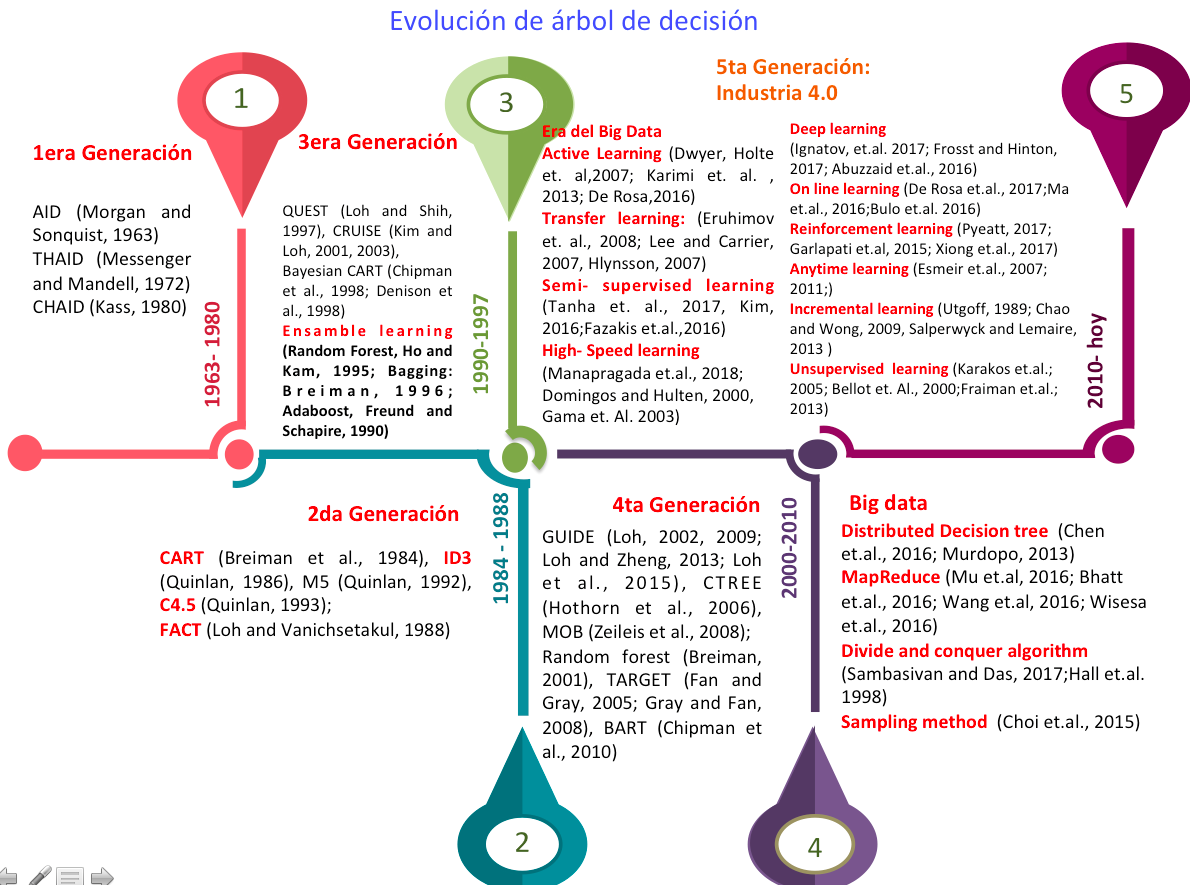
\includegraphics[height=11.5cm]{evulucion}
\caption{Evoluci�n del algoritmo de �rbol de decisi�n.}
\label{fig:evol}
\end{figure}


\subsection{Primera Generaci�n}

Incluye la descripci�n del algoritmo AID \cite{morgan1963problems}, THAID \cite{messenger1972modal}, y el CHAID \cite{kass1980exploratory}.  Esta generaci�n se inici� con �rboles de decisi�n para variables continuas (regresi�n), ajusta un modelo constante paso a paso por una divisi�n recursiva de los datos en dos subgrupos (nodos), con divisiones de la forma ``$X \leq c$'' o `$`X \in A$''. \par

\begin{figure}[ht]
\centering
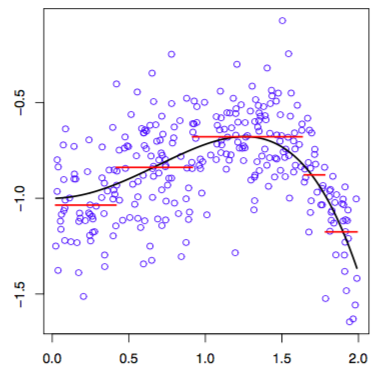
\includegraphics[height=7cm]{gen1}
\caption{Ajuste de primera generaci�n}
\label{fig:gen1}
\end{figure}

Para esto, se defini� el termino impureza (de cada nodo), \textbf{impureza} $\phi (t) = \sum_{i\in t} (y_i - \hat{y})$, un ejemplo de este ajuste se ve en la figura \ref{fig:gen1}. Aunque existen otros algoritmos que tambi�n pueden clasificar (THAID) o que mejoran la velocidad (CHAID).\par

\subsection{Segunda Generaci�n}

En esta generaci�n aparece el algoritmo \textbf{C}lassification \textbf{A}nd \textbf{R}egression \textbf{T}rees (CART) descrito por Breiman et. al. \cite{breiman85stone}.  Este algoritmo CART, usa la busqueda greedy utilizada en AID y THAID con otras adiciones:\par

\begin{enumerate}
	\item Los �rboles generados son podados en lugar de tener reglas de paro.
	\item Los �rboles son seleccionados por validaci�n cruzada.
	\item Se puede agregar un costo para las clasificaciones erroneas o para clases desbalanciadas.
	\item Se manejan los valores perdidos por particiones surrogadas.
	\item Se utilizan scores de importancia de las variables usadas para detectar el enmascaramiento.
	\item Particiones lineales $\sum_i a_i x_i \leq c$ se obtienen al azar (RPART ), es una implementaci�n de CART en R.
\end{enumerate}


Adem�s Quinlan inicia su prol�fica descripci�n de diferentes �rboles de decisi�n con el algoritmo ID3 \cite{quinlan1986induction}, M5 \cite{quinlan1992learning} y C4.5 \cite{quinlan2014c4}. En la tabla \ref{tab:carac}  se pueden observar las caracter�sticas que distinguen los diferentes algoritmos. En la figura \ref{fig:entrena} se puede ver como se clasifica una nueva observaci�n, mediante las reglas obtenidas de los datos de entrenamiento.

El algoritmo ID3 recibi� este nombre por que fue el tercero en procedimientos de identificaci�n de series. Fue realizado con la intenci�n de ser usado para datos nominales (no ordenados). Si el problema involucra variables con valor real, ellos son primero convertidos en intervalos, cada intervalo es tratado de forma no ordenada nominal. Cada split tiene un factor de rama de Bj, donde B, es el numero de atributos discretos de bins de la variable j escogida para la partici�n. En la practica, rara vez los datos son binarios as� que la impureza de la raz�n de ganancia debe ser usada. Estos �rboles tienen sus n�meros de niveles igual a el n�mero de variables ingresadas. El algoritmo continua hasta que todos los nodos son puros o no hay mas variables para particionar. No hay poda en las presentaciones est�ndar del algoritmo.

\begin{table}
\centering
\begin{tabular}{|p{1.8cm}|p{2cm}|p{2cm}|p{2cm}|}
\hline
& ID3 & C4.5 & CART\\ \hline
Criterio de Partici�n & Ganancia de informaci�n & Raz�n de Ganancia & Towing Criteria \\ \hline
Atributo & Categ�rico & Categorico y Num�rico & Categ�rico y Num�rico \\\hline
Valores Perdidos & No maneja & Maneja & Maneja \\ \hline
Poda & No & Basado en error & Costo de Complejidad \\ \hline
Outlier & No maneja & No maneja &Maneja \\ \hline
\end{tabular}
\caption{Caracter�sticas de los algoritmos de la 2da generaci�n}
\label{tab:carac}
\end{table}

\begin{figure}[h]
\centering
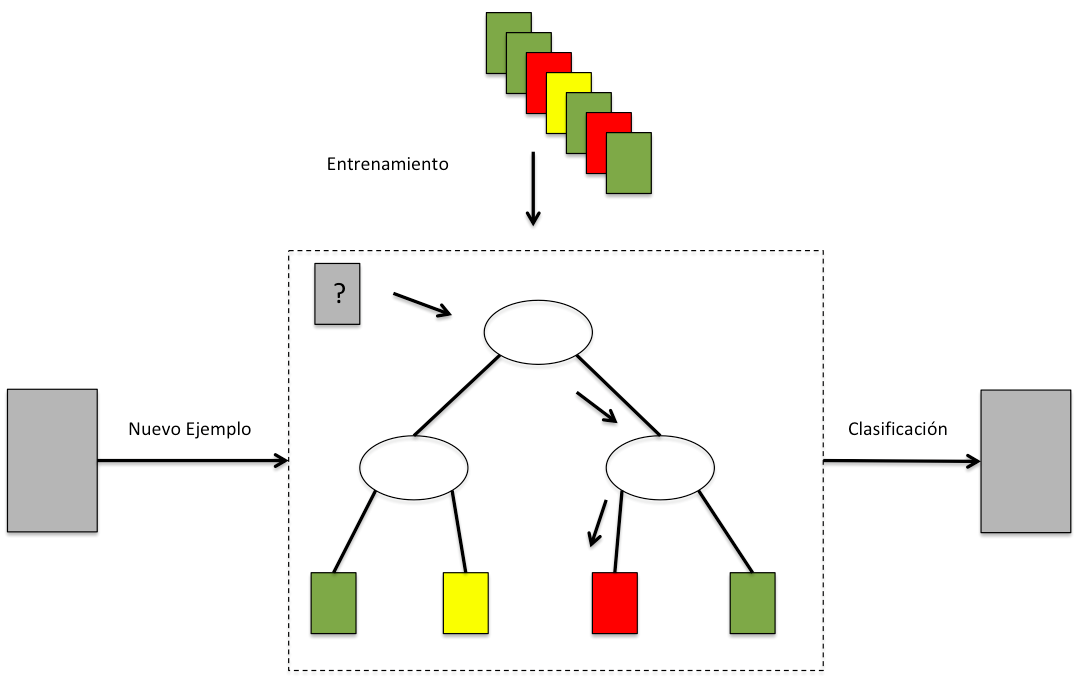
\includegraphics[height=7.5cm]{entrenamiento}
\caption{Clasificaci�n mediante algoritmos de la 2da generaci�n}
\label{fig:entrena}
\end{figure}
\newpage

\subsection{Tercera Generaci�n}

En 1997, la aparici�n del algoritmo \textbf{Q}uick, \textbf{U}nbiased and\textbf{E}fficient \textbf{S}tatistical \textbf{T}ree(QUEST) descrito por Loh y Shih \cite{loh1997split}, inicia la tercera generaci�n de algoritmos. Este algoritmo es el primero sin tener sesgo de selecci�n.  Se enlista algunas de sus principales caracter�sticas:\par

\begin{enumerate}
	\item Usa ANOVA y tablas de contingencia con pruebas $\chi^2$ para la selecci�n de variables.
	\item Mezcla clases en dos superclases para tener selecciones binarias.
	\item Usa el an�lisis discriminante cuadratico para encontrar el punto de partici�n.
	\item Usa imputaciones de datos mediante el promedio de los nodos.
	\item Poda con el m�todo CART.
\end{enumerate}

Estas caracter�sticas son similiares a las encontradas en el algoritmo \textbf{C}lassification \textbf{R}ule with \textbf{U}nbiased \textbf{I}nteraction \textbf{S}election and \textbf{E}stimation, CRUISE (desarrollado por Hyunjoon kim y Wei-Yin Loh \cite{kim2001classification} \cite{kim2003classification}), en el sentido de que utilizan la prueba de $\chi^2$ para la partici�n de variables y utiliza el an�lisis descriminante lineal para encontrar los puntos en donde partir. Sin embargo tiene otras que lo diferenc�an:\par

\begin{itemize}
	\item Particiona cada nodo en tantos subnodos como el n�mero de clases en la variable respuesta.
	\item Tiene un sesgo negligible en la selecci�n de variables.
	\item Tiene m�ltiples v�as de lidiar con valores perdidos.
	\item Puede detectar interacciones locales entre pares de variables predictoras.
\end{itemize}


\begin{figure}[h]
\centering
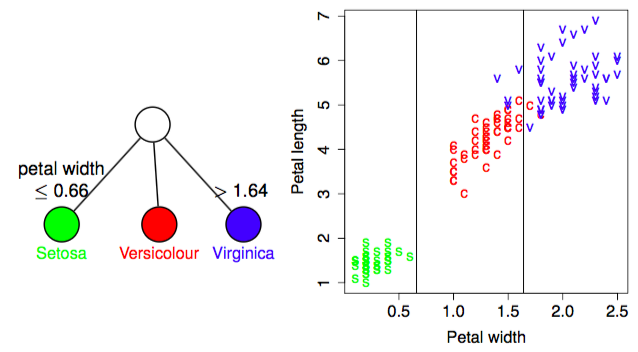
\includegraphics[height=6cm]{cruise}
\caption{Ejemplo de el �rbol de decisi�n CRUISE}
\label{fig:cruise}
\end{figure}

Un ejemplo de este �ltimo algoritmo se muestra en la figura \ref{fig:cruise}.

\subsection{Cuarta Generaci�n}

Este mismo autor Loh, publica el algoritmo GUIDE (cuarta generaci�n) que continua basandose en pruebas de significancia en el paso de dividir un nodo. Utiliza la prueba de $\chi^2$. El pseudoc�digo de este algoritmo  se describen a continuaci�n \cite{loh2011classification}:\par

\begin{tcolorbox}[title =  \centering Pseudoc�digo del algoritmo GUIDE, title filled]
\begin{enumerate}
\item Inicia en el nodo ra�z.
\item Para cada variable ordenada X, convierte a una no ordenada variable X' al agrupar sus valores en el nodo, dentro de un peque�o numero de intervalos. Si X es no ordenada, X' = X.
\item Realiza una prueba de $\chi^2$ de independencia para cada X`variable vs. Y en los datos del nodo y computa su probabilidad de significancia.
\item Escoge una variable X* asociada con el X' que tiene la probabilidad de significancia mas peque�a.
\item Encuentra la partici�n del conjunto \{X $\in$ S*\} que minimiza la suma de los indices Gini, y usalo para dividir el nodo en dos nodos mas peque�os.
\item Si el criterio de paro es alcanzado, termina, De otra forma, aplica los pasos 2 - 5 para alcanzar un nodo hijo.
\item Poda el �rbol con el metodo CART.
\end{enumerate}
\end{tcolorbox}

Este algoritmo puede dividir combinaciones de dos variables a la vez, y trata a los valores perdidos como una categor�a separada. Una comparaci�n entre los �ltimos algoritmos descritos se pueden ver en la tabla  \ref{tab:comp}.\par

\begin{table}[ht]
\centering
\begin{tabular}{cccc}\hline
\rowcolor{Gray} Caracter�stica & CRUISE & GUIDE & QUEST\\\hline
Partici�n no sesgada & $\sqrt[]{}$&$\sqrt[]{}$&$\sqrt[]{}$\\
Tipo de partici�n&$u,l$&$u,l$&$u,l$\\
Ramas/Partici�n & $\geq 2$ & 2 & 2 \\
Pruebas Interacci�n & $\sqrt[]{}$ &$\sqrt[]{}$ & \\
Poda & $\sqrt[]{}$ & $\sqrt[]{}$ & $\sqrt[]{}$\\
Costos (Usuario) & $\sqrt[]{}$ & $\sqrt[]{}$ & $\sqrt[]{}$ \\
Previo (Usuario) & $\sqrt[]{}$ & $\sqrt[]{}$ & $\sqrt[]{}$ \\
Ranking Variable & & $\sqrt[]{}$ & \\
Modelo de nodo &$c,d$& $c,k,n$& c \\
Bagging y Ensembles & &$\sqrt[]{}$& \\
Valores perdidos & i,s & m & i \\\hline
\end{tabular}
\caption{Comparaci�n de M�todos de clasificaci�n con �rboles. Una marca indica presencia de la caracter�stica}
\label{tab:comp} 
\end{table}

\subsection{Quinta Generaci�n}

En la quinta generaci�n se encuentra ya la era del big Data y la Industria 4.0. En ella se incluyen una gran cantidad de tipos de aprendizaje (learning) que tratan de superar los retos del Big Data. Se mencionar� brevemente el significado de los diferentes aprendizajes de esta generaci�n (tratando de no alejarse mucho del objetivo de esta tesis).

\subsubsection{Aprendizaje activo (Active Learning)}

Para describir el aprendizaje activo de una forma m�s comprensible, se debe contrastar con el aprendizaje pasivo (passive learning); que es el aprendizaje est�ndar, bien estudiado establecido en estad�stica y aprendizaje maquina). En el aprendizaje pasivo (ocasionalmente referido como aprendizaje supervisado), la meta es obtener un buen predictor de los datos etiquetados.  En el modelo de aprendizaje activo es un poco diferente a esto, ya que inicialmente los datos no tienen una etiqueta, el objetivo en este aprendizaje es el mismo que en el aprendizaje pasivo; sin embargo, en este tipo de aprendizaje esta permitido buscar una etiqueta respuesta para cualquier dato ingresado en los predictores \cite{hsu2010algorithms}.\par

\subsubsection{Aprendizaje de transferencia (Transfer learning)}

El aprendizaje de transferencia es dirige al proceso de adquisici�n de conocimiento (o habilidades) en el contexto de que una tarea acompa�ada de una subsecuente aplicaci�n del conocimiento para aprender nuevas tareas eficientemente \cite{won2007transfer}. Se debe considerar que las diferentes tareas descritas en este p�rrafo pueden diferentes relaciones como se ve en la figura \ref{fig:tareas} .


\begin{figure}
\centering
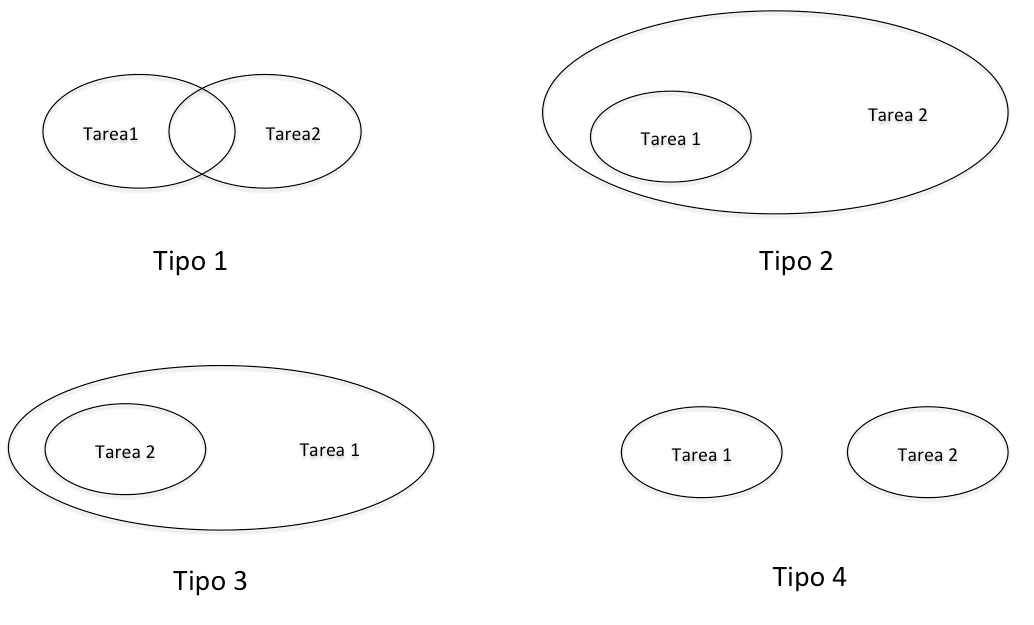
\includegraphics[height=7cm]{tareas}
\caption{Tipos de tareas en Aprendizaje de Transferencia}
\label{fig:tareas}
\end{figure}

El algoritmo de transferencia para �rboles de decisi�n, aprende  una nueva tarea u objetivo, de un modelo de decisi�n parcial, inducido por el ID3, que captura el conocimiento previo, de una tarea previa \cite{quinlan1986induction}. El algoritmo de �rboles de decisi�n de transferencia, consta de dos partes: 1) consise en identificar atributos que no ocurren en el �rbol de la tarea fuente y determina el orden en el que los nuevos atributos deben ser considerados; 2) consiste en aplicar transformaciones de la tarea fuente, para colocar los nuevos atributos en los lugares correctos, en conjunto con la etiqueta asociada.



\subsubsection{Aprendizaje semi-supervisado (Semi-supervised learning)}

Los m�todos semi-supervisados no usan solamente los datos etiquetados, sino que tambi�n usan los datos no etiquetados; esto con el motivo de combinar la informaci�n de los datos no etiquetados con los etiquetados para mejorar el desempe�o de la clasificaci�n \cite{tanha2017semi}. En este caso, el algoritmo base de aprendizaje es el �rbol de decisi�n y puede ser modificado  al combinar el algoritmo con por ej. el clasificador ingenuo de Bayes (Naive Bayes Tree Classifier).

% desde aqui %%%%5
\section{Algoritmo C4.5}

El algoritmo C4.5, el sucesor y refinado ID3, es el mas popular en cuanto a m�todos de "clasificaci�n" basados en �rboles. En el, las variables con valor real, son tratadas de la misma forma que en CART.  Con particiones multi-v�a, el algoritmo usa fundamentos heur�sticos para la poda del �rbol obtenido. Este algoritmo tiene la provisi�n para la poda basada en las reglas derivadas del mismo �rbol. Esto es mediante la v�a desde la ra�z al nodo final, si existen reglas redundantes, estas son eliminadas \cite{quinlan1993c4}.\par 

La construcci�n b�sica del algoritmo C4.5 es la siguiente:

\begin{itemize}
	\item Los nodos ra�z es el nodo mas arriba del nodo. El es considera todas las muestras y selecciona los atributos que son mas significantes.
	\item La informaci�n de la muestra es pasada a los nodos subsecuentes, llamados ``nodos de rama'' que eventualmente terminan en los nodos hoja que dan las decisiones.
	\item Las reglas son generadas mediante una ilustraci�n de la v�a de la ra�z a un hoja
\end{itemize}

C4.5 usa los valores de probabilidad para tratar a los datos perdidos, en lugar de asignar valores comunes de alg�n atributo. Aunque este algoritmo es de uso extendido tiene algunas limitantes \cite{mazid2010improved}:

\begin{itemize}
	\item Ramas vac�as: En caso que un nodo tenga 0 valores o valores cercanos a 0, no ayuda a construir reglas, sino que solo hace el �rbol mas complejo y grande.
	\item Ramas sin significado: Las variables discretas pueden ayudar a formar un �rbol de decisi�n pero no ayudan en la tarea de clasificaci�n llevando a tener un �rbol mas grande y al sobre ajuste.
\end{itemize}


\newpage

\section{Algoritmo C5.0}

El algoritmo C5.0 es un algoritmo relativamente nuevo basado en su antecesor C4.5 (desarrollado por  Quinlan) introduce nuevas tecnolog�as que incluyen el boosting y un �rbol de decisi�n sensible a una funci�n de costos. \cite{pang2009c5}
Este algoritmo es una extensi�n de C4.5 que a su vez es una extensi�n del ID3, este algoritmo es uno que puede aplicar en el concepto del big data ya que es mejor que el C4.5 en cuanto a la velocidad, memoria y eficiencia.\cite{brijain2014survey}

Un modelo C5.0 esta basado en la teor�a de la informaci�n y trabaja separando el conjunto de datos en multiples sub muestras.\cite{golmah2014efficient}

Similar al algoritmo de Adaboost, el boosting en C5.0 es una mejora importante. Esta basado en el c�lculo de un peso ("weight", en ingl�s) el cual se incrementa con la influencia en la muestra. El peso es ajustado en cada iteraci�n, con cada nueva muestra. El hecho de enfocarse a las muestras con peor clasificaci�n dada por el �rbol de decisi�n anterior hace que estas muestras tengan un mayor peso. % revisar las bibliograf�as.
Este m�todo de hacer �rboles de decisi�n es muy robusto para manejar los datos faltantes y grandes cantidades de ``inputs'' al modelo.


\section{�rbol de decision con vista hacia adelante (Look Ahead Decisi�n Tree)}

Aunque algoritmos de �rboles de decisi�n  descritos anteriormente son muy populares (como C4.5), este tipo de algoritmos basados en un abordaje �vido (``greedy''), tienen algunos inconvenientes,  por ejemplo las particiones tempranas (o nodos) o anteriores pueden afectar los nodos subsecuentes, llevando a: 1) parada temprana del �rbol (por encontrar un �ptimo local), 2) puede afectar la soluci�n final \cite{breslow1997simplifying}.\par

Una de las posibles alternativas es la utilizaci�n de el paso hacia adelante para escoger mejores particiones, poniendo atenci�n la efectividad futura (esto es suprime el efecto del horizonte). Aunque se piensa que puede mejorar la efectividad del algoritmo, algunos autores muestran la complejidad del �rbol resultante y que tal vez pudiera afectar la exactitud \cite{elomaa2005look} \cite{elomaa2003lookahead}\cite{murthy1995lookahead}.




\section{�rbol de Decisi�n Sensible a Costos (Cost Sensitive Decision Tree)}

La clasificaci�n en el contexto del aprendizaje maquina, maneja el problema de predecir la clase $y_i$ del conjunto de ejemplos $S$, dado sus $k$ variables. El objetivo es construir una funci�n $f(S)$ que prediga las $c_i$ clases de cada ejemplo usando las variables $X_i$. Esto pensando que  los diferentes errores de clasificaci�n tienen el mismo costo. Los m�todos que usan diferentes costos de error de clasificaci�n se conocen como clasificadores costo sensibles; los diferentes tipos de algoritmos se presentan en la figura \ref{fig:cs} \cite{bahnsen2015novel} .

\begin{figure}[h]
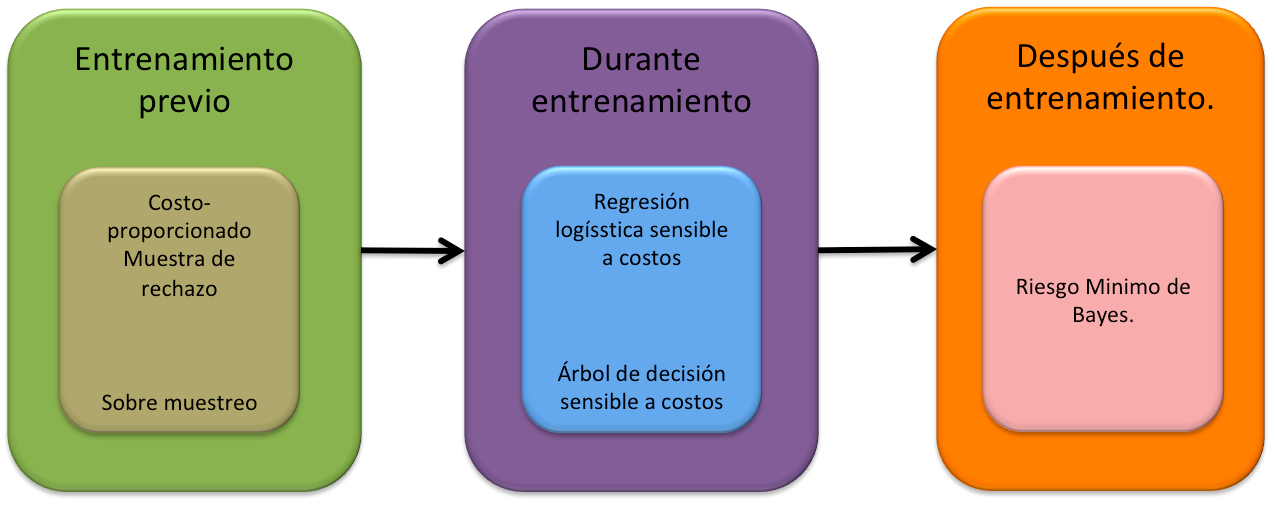
\includegraphics[height=6cm]{cs}
\caption{Algoritmos Sensibles a Costos}
\label{fig:cs}
\end{figure}

En el modelo propuesto por Correa Bahnsen , el criterio de partici�n es usado durante la construcci�n del �rbol de decisi�n. En lugar de utilizar criterios ya conocidos  como el Gini o entrop�a para el error de clasificaci�n, el costo definido: $Cost = \sum_{i=1}^{N} Costo_i$ para cada nodo es calculado y la ganancia de usar cada partici�n evaluada como el decremento en total de los ``ahorro'', definido como:  $Ahorro = \frac{Costo_i - Costo}{Costo_i} $.










\section{Algoritmo Utilizado:  �rbol de Decisi�n Sensible a Costos y con Mirada Adelante Generalizado}

Despu�s de la revisi�n de literatura m�dica y de los diferentes algoritmos existentes de �rboles de decisi�n, se tienen en mente diferentes problemas a la hora de realizar el an�lisis de este tipo de datos. Y estos incluyen:

\begin{enumerate}
\item Datos desbalanceados. Los grupos de las diferentes etiquetas no son iguales.
\item Posible error al seleccionar de variables. Siendo los datos de muy alta dimensionalidad, se puede presentar la ocasi�n de que la selecci�n de determinada variable pueda hacer crecer un �rbol con una tendencia a la mala clasificaci�n de pacientes.
\end{enumerate}

Por estos problemas se decide proponer un algoritmo que incluya la soluci�n (al menos parcial) de estos problemas: el Algoritmo Cost Sensitive Look Ahead Decision Tree. 

En este algoritmo se utiliza el criterio de informaci�n basado en la reducci�n de la entrop�a, siempre tomando en cuenta primeramente a la variable que maximiza esta reducci�n $G(k,l)$.

\begin{itemize}
\item $(k^*,\tau^*) = \text{argmax}_{k,\tau} G(k,\tau) $

\item Donde $G(k,\tau) =  E_{antes} - E_{despues}$.
\item $E$ denota la entrop�a, que es una medida de incertidumbre en los datos.

\item $E_{antes}$ y $E_{despues}$, denotan la entrop�a antes y despu�s de la partici�n.\par

\item $E_{antes} = E(D) =  \sum^m_{i=1} f(w_i,D) p(c_i,D) log_2 (p(c_i,D))$

\item $E_{despues} = \frac{|D_l (k,\tau)|}{|D|} E(D_l(k,\tau)) + \frac{|D_r(k,\tau)|}{|D|} E(D_r(k,l)) $

\item Donde D denota conjunto de entrenamiento, $C = \{c_1,c_2,\cdots,c_m\}$, denota el indice nivel de clase,
\item $D = \{(\textbf{v},y)\}$, $\textbf{v} = \{v_1, v_2,\cdots, v_M\} $ 
\item $\text{ es matriz de caracter�sticas,}$ $y\text{ pertenece al nivel }\\\text{de clase de cada muestra}$.

\item Tuple $(k,\tau)$ divide el conjunto de entrenamiento $D = \{(\textbf{v},y)\}$ en dos subconjuntos : 
\begin{itemize}
\item $D_l(k,\tau) = \{(\textbf{v},y) | v_k \leq \tau$\\
\item $D_r(k,\tau) = D\textbackslash D_l (k,\tau) $
\end{itemize}
\item $E(D_l(k,\tau)) =  \sum^m_{i=1} f(w_i,D_l) p(c_i,D_l) log_2 (p(c_i,D_l))$\\
\item $E(D_r(k,\tau)) =  \sum^m_{i=1} f(w_i,D_r) p(c_i,D_r) log_2 (p(c_i,D_r))$
\end{itemize}
\newpage

A esta forma de particionar los datos, se le puede sumar la posibilidad de agregar un peso a eventos de errores de clasificaci�n. Esto es hacer costo sensible al algoritmo, se puede ver en la siguiente tabla de contingencia que los errores que deben ser pesados (y disminuidos) son los falsos positivos y falsos negativos.
\vspace{2cm}
\begin{table}[h]
\centering
\begin{tabular}{c|c|c}
& Actual Positivo & Actual Negativo \\
Predicho positivo & $C_{TP_{i}}$ & $C_{FP_{i}}$\\
Predicho Negativ & $C_{FN_{i}}$ & $C_{TN_{i}}$
\end{tabular}
\caption{Matriz Costos de clasificaci�n\cite{bahnsen2015ensemble}}
\end{table}
\vspace{2cm}


\begin{tcolorbox}[title = �rbol de decisi�n sensible a costos, title filled]
$f(w_i,D) = \frac{\sum^m_{i=1,c\neq i}|D(c_i)|}{|D|}$\\~\\ $|D(c_i)| =$ \# de observaciones  en D pertenecientes a clase $c_i$.
$f(w_i,D) = 1 \forall i $ para �rboles de decisi�n no sensibles a costo 
\end{tcolorbox}
\newpage


\section{Forma de evaluar la efectividad de los �rboles de decisi�n}

Se decide agregar esta secci�n de "Forma de evaluaci�n de la efectividad de los �rboles de decisi�n" para tener una mayor conocimiento en las definiciones de los t�rminos utilizados.  La mayor�a de los t�rminos son utilizados en la literatura m�dica y su entendimiento por los mismos profesionales es claro; sin embargo no necesariamente lo es para los profesionales de las otras ramas.  Sin mas se describen los t�rminos

Uno de los t�rminos mas importantes es el de la exactitud (\textbf{accuracy}, en ingl�s). Este define el porcentaje sujetos que son correctamente clasificados. Se incluyen los adecuadamente clasificados como ej. positivo o negativo.

Otro de los t�rminos utilizados en las pruebas medicas es la sensibilidad (\textbf{sensitivity}, en ingl�s) que es la habilidad de una prueba de dar un resultado positivo en casos verdaderos de enfermedad. La especificidad (\textbf{specificity}, en ingl�s) es la habilidad de dar un resultado negativo en caso de que la enfermedad este ausente. Ambas son probabilidades y son expresadas en porcentaje. Para calcular ambas caracter�sticas de las pruebas se determinan los casos verdaderos y falsos positivos; esto es: cuantos de los sujetos son clasificados correcta e incorrectamente.  Podemos observar la formula de ambas a continuaci�n:

\begin{equation}
\text{Sensibilidad } = \frac{TP}{TP + FN}
\end{equation}

\begin{equation}
\text{Especificidad } = \frac{TN}{TN + FP}
\end{equation}

Otros t�rminos que se agregaron a la evaluaci�n del modelo son las probabilidades post test. Estas probabilidades son por as� decirlo, la inversa de la sensibilidad y la especificidad. Y se refieren a la probabilidad de que un paciente tenga una enfermedad ya que tiene la prueba positiva (\textbf{valor predictivo positivo}) o de que no la tenga si tiene una prueba negativa (\textbf{valor predictivo negativo}). Las formulas de estas probabilidades se muestran a continuaci�n\cite{indrayan2017medical}:

\begin{equation}
\text{Valor predictivo positivo } = \frac{TP}{TP + FP}
\end{equation}

\begin{equation}
\text{Valor predictivo negativo } = \frac{TN}{TN + FN} 
\end{equation}

Se hace menci�n tambi�n que en la secci�n de anexo, se tendr� la oportunidad de revisar un poco sobre el tema de regresi�n log�stica y la selecci�n hacia adelante de variables (Forward selection), as� tambi�n se revisar� un poco sobre la t�cnica de bootstrap. 


\chapter{Aplicaci�n de los �rboles de decisi�n en el s�ndrome metab�lico}

\section{Origen de los datos}

En esta secci�n se detalla con mas profundidad la obtenci�n de las bases de datos utilizadas en este trabajo. Los resultados ser�n discutidos en el texto y se mostrar�n en las tablas. Se debe comentar que de las bases de datos obtenidas en los diferentes estudios, se computaron las metas caracter�sticas para cada una de las bases de datos. Estas meta caracter�sticas, refieren a nuevas variables que son construidas de las bases de datos mediante combinaciones lineales de las variables. Estas combinaciones lineales son obtenidas mediante el uso de operaciones aritm�ticas b�sicas (suma, resta multiplicaci�n y divisi�n). En las tablas donde se refiera a los datos obtenidos mediante meta caracter�sticas se les agrega un s�mbolo de (+) cuando los datos son analizados en crudo m�s las meta caracter�sticas. 

\subsection{H�gado graso no alcoh�lico y retinopat�a.}

La base de datos para el el estudio de el H�gado graso no alcoh�lico y retinopat�a se obtuvo de un proyecto llevado acabo en el Hospital General de M�xico. Se dise�� un estudio transversal, observacional, comparativo y prolectivo en el que completamos cuatro grupos de pacientes: 

\begin{enumerate}
\item Pacientes con EHNA y obesidad (IMC>30), 
\item Pacientes con EHNA sin obesidad  (IMC<25), 
\item Pacientes sin EHNA con obesidad 
\item Pacientes sin EHNA sin obesidad
\end{enumerate}
Estos grupos son desbalanceados (tama�os de muestra diferentes), y con los siguientes criterios de:
Inclusi�n: 
\begin{itemize}
\item Edad: 18-45 a�os
\item Hombres y mujeres por igual
\item IMC para los obesos: >30; para los no obesos: 20 -25
\end{itemize}

Exclusi�n:
\begin{itemize}
\item Pacientes con h�bito de fumar que tengan �ndice tab�quico>1.
\item Ingesti�n de alcohol >10g a la semana.
\item Pacientes con historia cl�nica de Diabetes, Hipertensi�n, Insuficiencia renal cr�nica, c�ncer enfermedad inflamatoria o infecciosa aguda o cr�nica.
\item Pacientes que estuvieran tomando medicamentos hepatot�xicos.
\item Pacientes que no son conocidos por alguna de las condiciones del inciso anterior pero que durante el examen f�sico o los resultados de laboratorios fueran diagnosticadas. 
\item Pacientes con alguna patolog�a ocular que impida visualizaci�n de fondo de ojo o presencia de alguna otra retinopat�a asociada.
\item Pacientes embarazadas.
\item Pacientes que no acepten participar.
\item Pacientes que hayan aceptado participar que no acudan a las citas programadas para medici�n de variables.
\end{itemize}

\subsubsection{Escala de medici�n de las variables.}

Acorde al tratamiento estad�stico las variables pueden modificarse como predictoras (independientes) o predichas (dependientes). En general las podemos clasificar en los siguientes grupos:\par
Variables independientes (ver anexo1): talla, peso, �ndice de masa corporal, obesidad, cintura, porcentaje de grasa corporal, presi�n arterial, curva de tolerancia a la glucosa, �ndice de sensibilidad a la insulina por Matsuda \cite{matsuda1999insulin},colesterol total, triglic�ridos, colesterol de alta densidad (c-HDL), colesterol de baja densidad (c-LDL). \par
Variables dependientes (ver anexo 1): Factor estimulante de colonias de granulocito-macr�fago (GM-CSF), Interfer�n Gama (IFN-?) , Interleucina 10 (IL-10), Interleucina 2 (IL-2), Interleucina 4 (IL-4), Interleucina 6 (IL-6),Interleucina 8 (IL-8), Factor de necrosistumoral alfa (TNF $\alpha$), Prote�na C Reactiva. Di�metro arteriolar y venular de la retina,  cruces arteriovenosos, relaci�n arteriovenular, tortuosidad, alanino amino transferasa (ALT), glutamino amino transferasa (AST).\par
Se incluyeron a pacientes de la consulta externa del Hospital General de M�xico (febrero - agosto 2012). Posterior a aplicar criterios de inclusi�n y exclusi�n se citaron  a los pacientes un �nico d�a de acuerdo a las preferencias y conveniencias del mismo. Previo firma de consentimiento informado se realiz� una breve historia cl�nica donde se interrog� sobre los antecedentes de tabaquismo, alcoholismo, consumo de medicamentos hepatot�xicos, hepatitis, hipertensi�n, diabetes, enfermedades cr�nicas o agudas infecciosas; historia familiar de diabetes, obesidad e hipertensi�n. 
Se tom� presi�n arterial, aplicando los criterios de la JNC7 para descartar hipertensi�n, peso, talla y c�lculo de IMC, as� como realizaci�n de impedancia bioel�ctrica con aparato RJL, modelo Quantium IV (EUA).\par
La toma de muestra para an�lisis de par�metros bioqu�micos se realiz� de la siguiente manera: el personal de enfermer�a calificado coloc� un punzocat de12-16Gen venas superficiales de antebrazo. Se tom� una muestra sangu�nea basal, de la cual se obtuvo suero para la medici�n de: glucosa, urea, creatinina, �cido �rico, colesterol total, colesterol HDL, colesterol LDL, Triglic�ridos, Prote�na C reactiva, AST, ALT; los que se analizaron con un equipo Beckman automatizado . Tambi�n se obtuvo suero para medici�n de insulina la que se analiz�  por m�todo de ELISA con el equipo Multiskan Ascent V1.24 (USA).El coeficiente de variaci�n de las replicaciones (CV\%) oscil� entre 1.81 y 2.94\%.  Adem�s se midi� la concentraci�n  en suero de  IL 2, IL4, IL6, IL8, IL10, IFN, GM-CSF, TNF? a trav�s de ELISA m�ltiples con equipo Bioplex-ProTMAssays (Bio Rad, USA). El coeficiente de variaci�n de las repeticiones (CV\%) fue el siguiente: GM-CSF: 19, IFN-$\gamma$: 15, IL-10: 8, IL-2: 12, IL-4: 11, IL-6: 16, IL8: 17, TNF$\alpha$: 4 .\par
Adem�s se realiz� curva de tolerancia a la glucosa oral con 75 gr de glucosa anhidra, se tomaron muestras sangu�neas a los 30, 60, 90 y 120 minutos.\par
Para la fotograf�a de fondo de ojo se administr� el midri�tico TP (tropicamida). La fotograf�a digital se realiz� con la c�mara Visucam NM/SA n�mero 07740. Las fotos fueron tomadas con foco en papila central, temporal, nasal y se realiz� una reconstrucci�n de 7 im�genes en una sola por computadora. Estas im�genes fueron analizadas de manera ciega, al azar por el retin�logo que mostr� a trav�s de la prueba de concepto mayor correlaci�n cl�nica intraobservador (ver marco te�rico). El retin�logo consider� como fondo de ojo anormal ( FOa) la presencia de al menos 2/3 de los siguientes caracter�sticas cl�nicas:  p�rdida de la relaci�n arteria-vena, tortuosidad y cruces arteriovenosos patol�gicos.\par
Finalmente se realiz� en los pacientes ultrasonido de h�gado y v�as biliares con equipo Voluson Pro V de General Electric (USA), con un transductor de 3.5MHz, para determinar la presencia de EHNA de manera cl�nica apreciativa de acuerdo a la imagen observada por operador con base a tres par�metros \cite{charatcharoenwitthaya2007role} \cite{pluma2009higado}: 1) Ecotextura: la esteatosis se observa como un incremento de  la ecogenicidad en ecos muy finos y condensados, con apariencia de ?h�gado brillante?. 2) Aumento en la atenuaci�n: a mayor atenuaci�n mayor dificultad de penetrar el h�gado, lo que causa oscurecimiento posterior y p�rdida de la definici�n del diafragma, lo que tambi�n resulta en un ri��n relativamente hipoecoico. 3) Vasos hep�ticos: disminuye la visualizaci�n de las venas porta y hep�ticas, dando lugar a una apariencia blanda o sin caracter�sticas del h�gado, por la compresi�n del par�nquima lleno de grasa; estos hallazgos hacen dif�cil la diferenciaci�n entre esteatosis hep�tica difusa y otras enfermedades parenquimatosas difusas. Adem�s se calcul� la distribuci�n del tono gris de los pixeles en el l�bulo derecho del h�gado y se compar� con la densidad en pixeles del ri��n derecho, con lo que se calcul� el �ndice:\par

 
\[\frac{\hat{x}_{pix}\text{hep�tico}}{\hat{x}_{pix}\text{renal}}, \]

donde el numerador corresponde al promedio de grises de los pixeles registrados en el h�gado; y el denominador al promedio de los mismos en el ri��n correspondiente


\subsection{Diabetes mellitus}

Este estudio fue llevado a cabo en el Departamento de Endocrinolog�a del Hospital Universitario ``Jos� E. Gonz�lez'', a los pacientes que acudieron a la consulta externa, se les invito a participar a nuestro estudio previo consentimiento informado. Se  incluyeron 124 pacientes los cuales fueron categorizados de la siguiente forma:\par

\begin{figure}
\centering
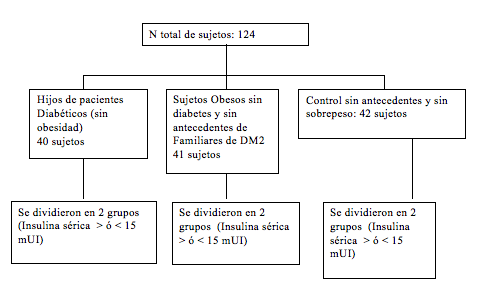
\includegraphics[height=7cm]{hu_px}
\caption{Grupos de pacientes de donde se obtuvieron los datos para la predicci�n de Diabetes}
\end{figure}

Para este trabajo solo se incluyeron, los grupos de sujetos normales y de los sujetos con diabetes meliitus. Y fueron reclutados bajo los siguientes criterios de inclusi�n.\par

\begin{itemize}
\item Sujetos sin antecedentes de diabetes mellitus, no diab�ticos, sin sobrepeso (IMC <25kg/m2).
\item Sujetos con Diabetes mellitus
\end{itemize}

\subsubsection{Metodolog�a}
A los pacientes que cumplieron con los criterios de inclusi�n se les realizo una antropometr�a adem�s de la recolecci�n de muestra para la evaluaci�n bioqu�mica:

\subsubsection{Obtenci�n de muestras de sangre}
Previa firma de consentimiento informado se coloc� una canalizaci�n y se les tomaron muestras basales que incluyen: glucosa, perfil de l�pidos, insulina, acil carnitinas; aproximadamente se extrajeron 60 ml. de sangre. Posteriormente se les dar� 75g de glucosa y se les mantendr� en reposo en el �rea de Pruebas Din�micas de Endocrinolog�a. En el transcurso de la prueba se realizar� Curva de Tolerancia a la Glucosa de 2 horas. Al las dos horas de ingerido se repetir� la insulina, acilcarnitinas. Aproximadamente se extraer�n 20 ml adicionales de sangre, para un total de 80 ml. Las muestras ser�n enviadas al laboratorio correspondiente para an�lisis. Se remover� la canalizaci�n y se citar� al paciente para entrega de resultados de laboratorio y discusi�n de los hallazgos. Se tomar�n 2 tubos de sangre, los que ser�n guardados en congelador para su an�lisis posterior.\par

Glucosa Enzim�tica. M�todo de Trinder-Colorim�trico. La determinaci�n de la glucosa se realizara utilizando la glucosa oxidasa (GOD). La glucosa es oxidada por la GOD a acido glucur�nico y agua oxigenada. En otra reacci�n secuencial interviene la peroxidasa que une al p-hidroxibenzoato con 4-aminoantipirina formando un crom�geno con absorbancia m�xima de 505nm.\par

Acil carnitinas por espectrometr�a de masas en tandem. El espectr�metro de masas es un detector que identifica masas (peso) de mol�culas individuales y sus fragmentos. Lo detectado se presenta en una grafica; eje de las x representa las masas y el eje de las y la cantidad de iones. El espectr�metro tiene alta sensibilidad y especificidad y capacidad de multi an�lisis.\par


Insulina por Electro quimioluminiscencia.  Se realizan dos incubaciones en t�cnica de s�ndwich que duran en total 18 minutos. En la primera incubaci�n se ponen 20$^o$ de la muestra con un anticuerpo monoclonal biotinilado espec�fico anti-insulina y otro anticuerpo monoclonal espec�fico marcado con quelato de rutenio. La segunda incubaci�n incluye la adici�n de micropart�culas de estreptavidina, dando como resultado un complejo que se fija a la base s�lida por interacci�n entre la biotina y la estreptavidina. La mezcla se transfiere a un lector que por magnetismo separa la micro part�culas. Los elementos no fijados se eliminan. Se aplica una corriente el�ctrica definida y se produce una reacci�n de quimioluminicencia cuya emisi�n de luz se mide directamente con un fotomultiplicador. Los resultados se obtienen mediante curva de calibraci�n.\par

Hemoglobina glucosilada. Se basa en la inhibici�n de la inmunoaglutinaci�n de part�culas l�tex. Tras introducir el cartucho en la c�mara anal�tica del sistema DCA 2000, el resultado aparecer� en 6 minutos. En este an�lisis se determinan la concentraci�n de HbA1c, la concentraci�n de hemoglobina total y la relaci�n entre ambas, se reporta como porcentaje de hemoglobina A1c. \par
%\section{Implementaci�n}

\newpage
\section{H�gado graso no alcoh�lico (NAFLD)}

En esta secci�n se desarrolla la aplicaci�n de �rboles de decisi�n para la clasificaci�n de pacientes con h�gado graso no alcoh�lico (NAFLD). Se aplicaran los algoritmos descritos de C4.5, C5.0, look ahead y cost sensitive; as� como la reducci�n de dimensi�n con la regresi�n log�stica con paso adelante.

\subsection{Algoritmo C4.5 y C5.0}

Para resolver el problema de clasificaci�n de pacientes con h�gado graso no alcoh�lico, se utilizaron todas las variables reportadas (no solo las relacionadas a las acilcarnitinas). En la figura \ref{fig:c45_nafld} se puede observar como el modelo obtenido por el algoritmo C4.5 toma encuentra variables cl�nicas y bioqu�micas b�sicas como la circunferencia abdominal, glucosa de ayuno y triglic�ridos.

\begin{figure}[H]
\centering
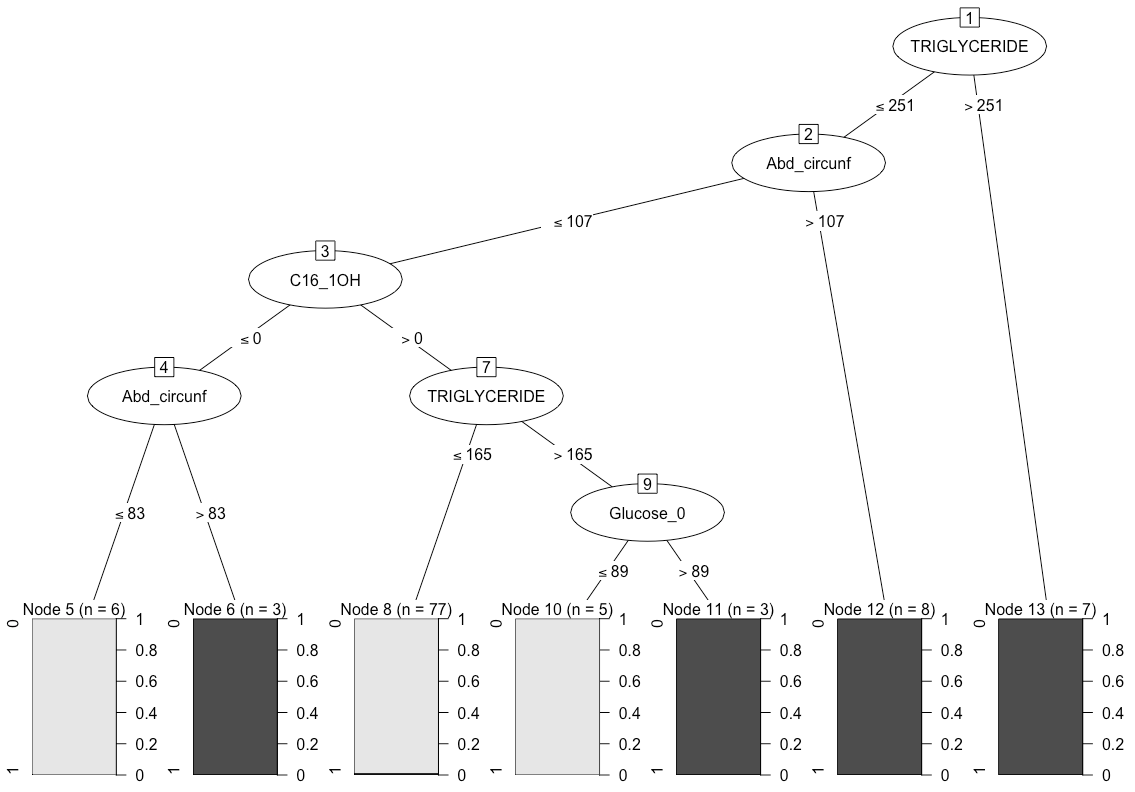
\includegraphics[width=10cm]{c45_nafld}
\caption{Modelo obtenido del algoritmo C4.5}
\label{fig:c45_nafld}
\end{figure}

El desempe�o de este modelo es bastante aceptable en general, teniendo un buen balance en cuanto a sensibilidad y especificidad. La exactitud del modelo es muy alta, 89.2\%, tabla \ref{tab:c45nafld} .



\begin{table}[H]
\centering
\begin{tabular}{||c||c||}
\hline \hline
Estad�stico & Valor \\\hline \hline
Exactitud & 89.2\% \\
Sensibilidad & 77.7\% \\
Especificidad & 94.7\% \\
V. Predictivo Positivo & 87.5\% \\
V. Predictivo Negativo & 90\% \\ \hline \hline
Validaci�n cruzada & \\\hline \hline
Exactitud & 97.6\% (IC 94.3\%, 100\%)\\
Sensibilidad & 91.8\% (IC 81.2\%, 100\%)\\
Especificidad & 100\% \\
V. Predictivo Positivo & 100\% \\
V. Predictivo Negativo & 97\% (IC 92.9\%, 100\%)\\ \hline \hline
\end{tabular}
\caption{Desempe�o de modelo obtenido por C4.5}
\label{tab:c45nafld}
\end{table}

\begin{figure}[H]
\centering
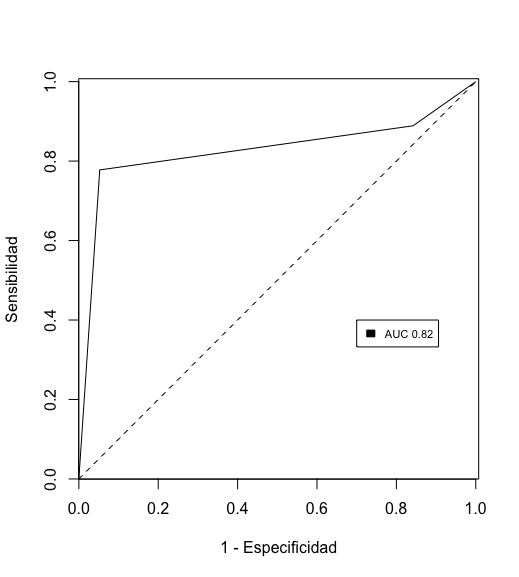
\includegraphics[width=7cm]{c45_auc_nafld}
\caption{AUC del modelo obtenido por C4.5}
\end{figure}

No se muestra el modelo obtenido con C5.0 ni su tabla de desempe�o porque es exactamente la misma que la obtenida por C4.5.

\subsection{Reducci�n de dimensiones realizado mediante regresi�n log�stica}

En la figura \ref{fig:c45_fs_nafld} se aprecia como las variables de peso, triglic�ridos y acilcarnitnas de cadena larga (C14 - C18) son fuertes predictores de la presencia de h�gado graso. El desempe�o de este modelo es muy competitivo y sigue caracterizandose por buena especificidad, tabla \ref{tab:esp_c4.5fs}.

\begin{figure}[H]
\centering
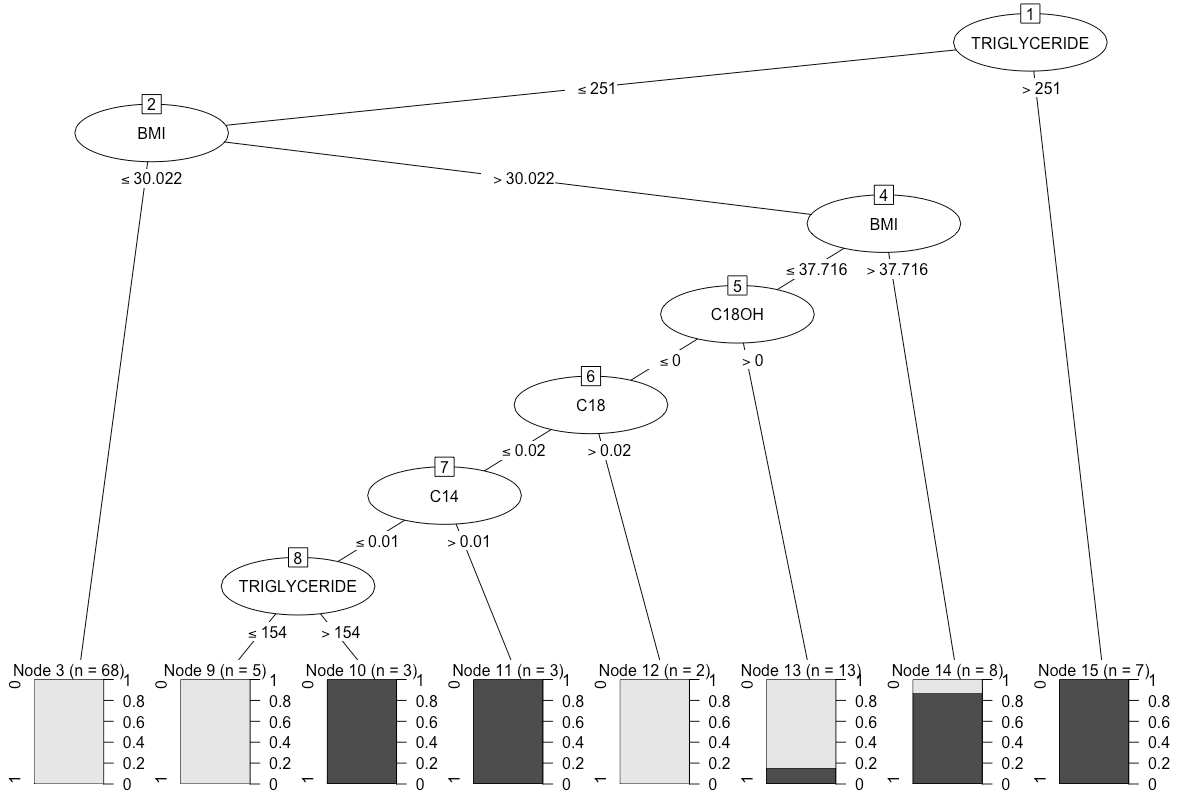
\includegraphics[width=10cm]{c45_fs_nafld}
\caption{Modelo obtenido mediante C4.5 y FS/LR}
\label{fig:c45_fs_nafld}
\end{figure}


\begin{table}[h]
\centering
\begin{tabular}{||c||c||}\hline\hline
Estad�stico & valor\\\hline \hline
Exactitud & 85.7\%\\
Sensibilidad & 77.7\%\\
Especificidad & 89.4\%\\
V. Predictivo Positivo & 77.7\% \\
V. Predictivo Negativo & 89.4\% \\ \hline \hline
Validaci�n cruzada & \\
Exactitud & 94.9\% (IC 78.1, 91.7)\\
Sensibilidad & 80\% (IC 65.8\%,94.1\%)\\
Especificidad & 87.4\% (IC 82.4\%, 92.5\%)\\
V. Predictivo Positivo & 66.6\% (IC 54.5\%, 78.7\%)\\
V. Predictivo Negativo & 92.2\% (IC 86.3\%, 98.1\%)\\ \hline \hline
\end{tabular}
\caption{Desempe�o de algoritmo C4.5 FS/LR}
\label{tab:esp_c4.5fs}
\end{table}

\subsection{Evaluaci�n del desempe�o mediante bootstrap}

Como en la secci�n anterior, describimos el resultado de la evaluaci�n de los modelos mediante bootstrap.


\begin{figure}[H]
\centering
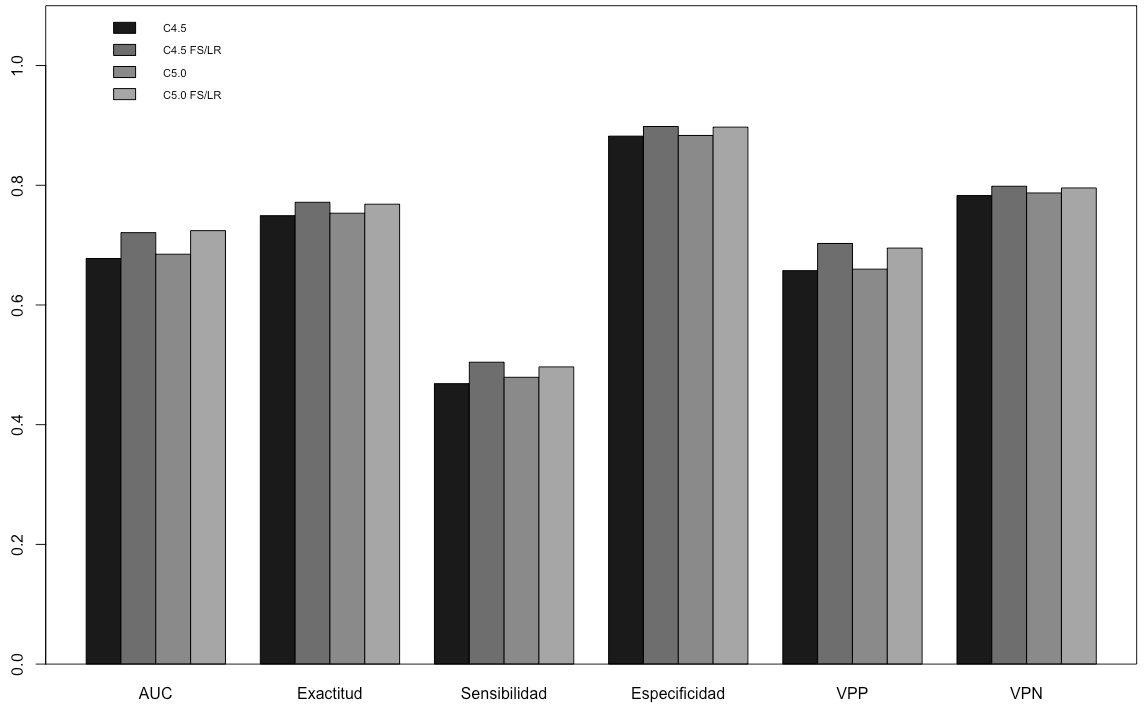
\includegraphics[width=10cm]{b_nafld}
\caption{Desempe�o de los algoritmos mediante bootstrap}
\label{fig:b_nafld}
\end{figure}

Como se muestra en la figura \ref{fig:b_nafld}, los algoritmos tienen una tendencia a ser muy espec�ficos y en este caso C4.5 y C5.0 en conjunto con FS/LR presentan la misma especificidad ya que se obtienen los mismos modelos.



\subsection{Aplicaci�n de �rbol de decisi�n costo sensible}

Como se observa en la tabla \ref{tab:cs_nafld}, el �rbol de decisi�n costo sensible puede incrementar de manera sobresaliente en comparaci�n a C4.5 y C5.0, pero no hay gran diferencia entre la exactitud derivada de diferentes costos.

\begin{table}[h]
\centering
\begin{tabular}{|c|c|c|}\hline
\begin{minipage}{.33\textwidth}
Costo (Estimado = NAFLD/ \\Actual = Normal) 
\end{minipage}
& \begin{minipage}{0.33\textwidth}
 Costo (Estimado = Normal/\\Actual = NAFLD) 
 \end{minipage}
 & Exactitud\\\hline
0.25 & 0.75 & 90.6  \\\hline
0.75 & 0.25 & 91.24  \\\hline
0.33 & 0.67 &  90.73 \\\hline
0.67 & 0.33 &  92.45  \\\hline
0.5 & 0.5 &  91.24 \\\hline
\end{tabular}
\caption{Resultados de clasificaci�n de NAFLD con diferentes costos}
\label{tab:cs_nafld}
\end{table}
\newpage
%
%
\subsection{Look Ahead Decision Tree.}

Como se muestra en la tabla \ref{tab:look_nafld}, este algoritmo no supera al anterior y de hecho empeora la clasificaci�n. Aunque si se utilizan dos nodos adelante para la clasificaci�n se mantiene con casi la misma clasificaci�n que los algoritmos base de C4.5 y C5.0.

\begin{table}[h]
\centering
\begin{tabular}{|c|c|c|c|}\hline
                  & Deep 1 & Deep 2 & Deep 3 \\ \hline
B = 0.01 & 78 &  84.6 & 78.7 \\\hline
B = 0.03 & 78.9& 77.4 & 76.7\\\hline
B= 0.06 & 78.6& 73.6 & 74.5\\\hline
B = 0.09 & 78.7& 80.9 & 79.6\\\hline
B = 0.1& 81.8& 82.4 & 77.3\\\hline
\end{tabular}
\caption{Resultados para clasificar pacientes con NAFLD con diferente beta (B) y diferente profundidad  (Deep) de vista hacia adelante.}
\label{tab:look_nafld}
\end{table}

\subsection{Meta caracter�sticas}

En este segmento se describe la aportaci�n de las meta caracter�sticas para la clasificaci�n de h�gado graso. Como se ve en la tabla \ref{tab:meta_c4.5_nafld}, El algoritmo C5.0 puede mejorar su clasificaci�n sobre todo con los datos generados de por el m�todo de suma. El resto no muestra un gran cambio.

\begin{table}[h]
\centering
\begin{tabular}{|c|c|c|}\hline
 				& C4.5 & C5.0  \\\hline
Suma & 83.9 &   92.8     \\\hline
Suma + & 83.9 &     92.8   \\\hline
Resta & 81.7	& 89.1      \\\hline
Resta + & 81  &    89.8      \\\hline
Multiplicaci�n & 83.9 &   87.8     \\\hline
Multiplicaci�n + & 83.9  &  87.8      \\\hline
\end{tabular}
\caption{Exactitud (\%) de los algoritmos con metacaracteristicas en NAFLD}
\label{tab:meta_c4.5_nafld}
\end{table}

En la tabla \ref{tab:meta_look_nafld1} se observa como el algoritmo costo sensible puede mejorar la clasificaci�n con practicamente cualquier costo y sin una predilecci�n entre el origen de los datos.


\begin{table}[H]
\centering
\begin{tabular}{|c|c|c|c|c|c|}\hline
 	Costos	& 0.25 - 0.75 & 0.75 - 0.25 & 0.33 - 0.67 & 0.67 - 0.33 & 0.5 - 0.5   \\\hline
Suma & 93.6 & 87.5   & 93.4 & 90 &  94.5  \\\hline
Suma + & 93.7  & 90.3  & 94.8 &91.2 &  92.7   \\\hline
Resta & 92.1	&  87.9 &89.2 & 90.2 &   91.2  \\\hline
Resta + & 92.5  & 91.4    & 90.7 & 91.4 & 90.5     \\\hline
Multiplicaci�n &89.4  & 93    & 90 & 93.6 & 89.7   \\\hline
Multiplicaci�n + & 92.3  & 95   &89.76 & 93.4 & 90.8   \\\hline
\end{tabular}
\caption{Exactitud (\%) de los algoritmos con metacaracteristicas con CSDT en NAFLD}
\label{tab:meta_look_nafld1}
\end{table}

Por otro lado, el algoritmo look ahead incrementa la exactitud en combinaci�n con las meta caracter�sticas originadas por resta y en Deep 2.Tabla \ref{tab:meta_look_nafld}

\begin{table}[H]
\centering
\begin{tabular}{|c|c|c|c|}\hline
                  & Deep 1 & Deep 2 & Deep 3 \\ \hline
Suma & 75.2   &  76.4  &  75.9 \\\hline
Suma + & 74.5  & 75   & 75.8     \\\hline
Resta & 84.6 & 90.4   &   86.7    \\\hline
Resta + &  82.3  &  85.4  & 83.1  \\\hline
Multiplicaci�n & 82.5   &  84    &   82.4 \\\hline
Multiplicaci�n + &  83.2  &  81  & 83.2  \\\hline
\end{tabular}
\caption{Exactitud (\%) de los algoritmos con metacaracteristicas con LADT previa selecci�n de variables en NAFLD (todos fueron con B = 0.1)}
\label{tab:meta_look_nafld}
\end{table}



%
%
%
\section{Diabetes mellitus}

En esta secci�n se aplican los diferentes algoritmos de �rboles de decisi�n para la clasificaci�n de sujetos con y sin diabetes mellitus tipo 2.\vspace{-1.cm}

\subsection{Algoritmo C4.5 y C5.0}

Los modelos resultantes de evaluar la informaci�n metabol�mica de los pacientes con diabetes mellitus tipo 2 se observan en las figuras \ref{fig:dm_j48} y \ref{fig:dm_c50}  .

\begin{figure}[H]
\centering
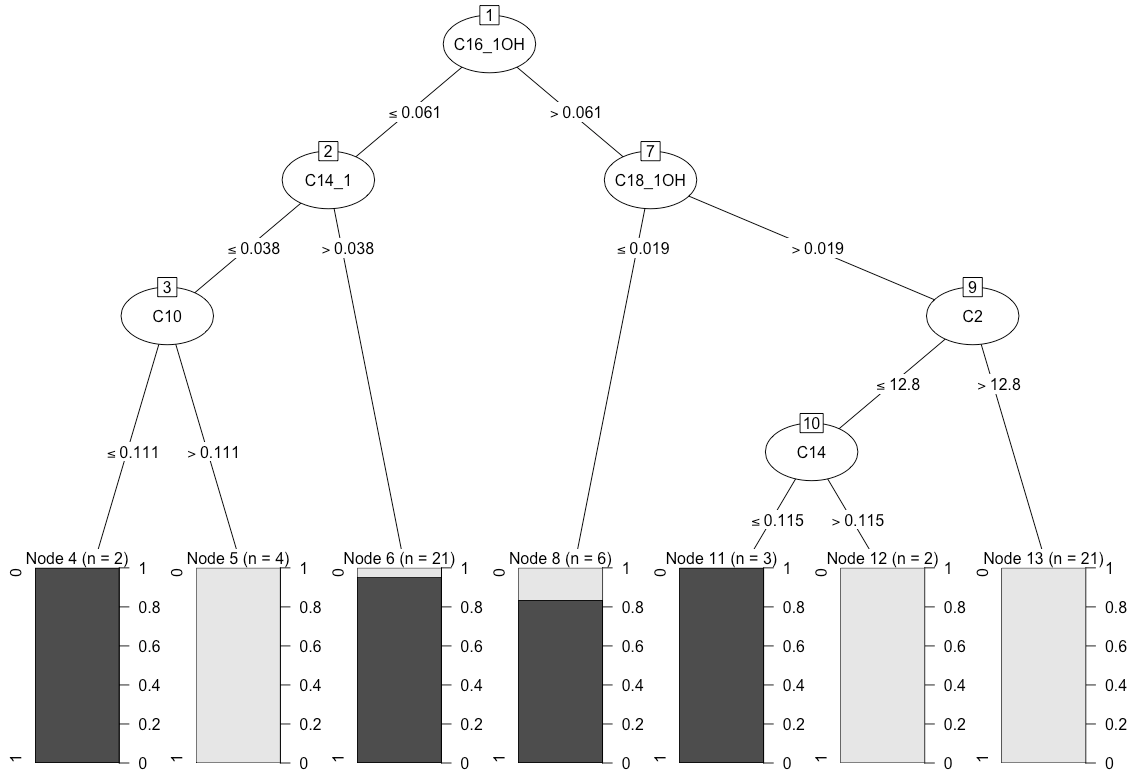
\includegraphics[width=12cm]{dm_j48}
\caption{�rbol obtenido el algoritmo C4.5}
\label{fig:dm_j48}
\end{figure}
Estos �rboles de decisi�n muestran como las variables explicativas relacionadas a las acilcarnitinas de cadena larga son muy importantes en la clasificaci�n de los pacientes con diabetes mellitus tipo 2. Ambos son muy parecidos en tama�o y en las variables tomadas en cuenta para clasificar.\par
\begin{figure}[H]
\centering
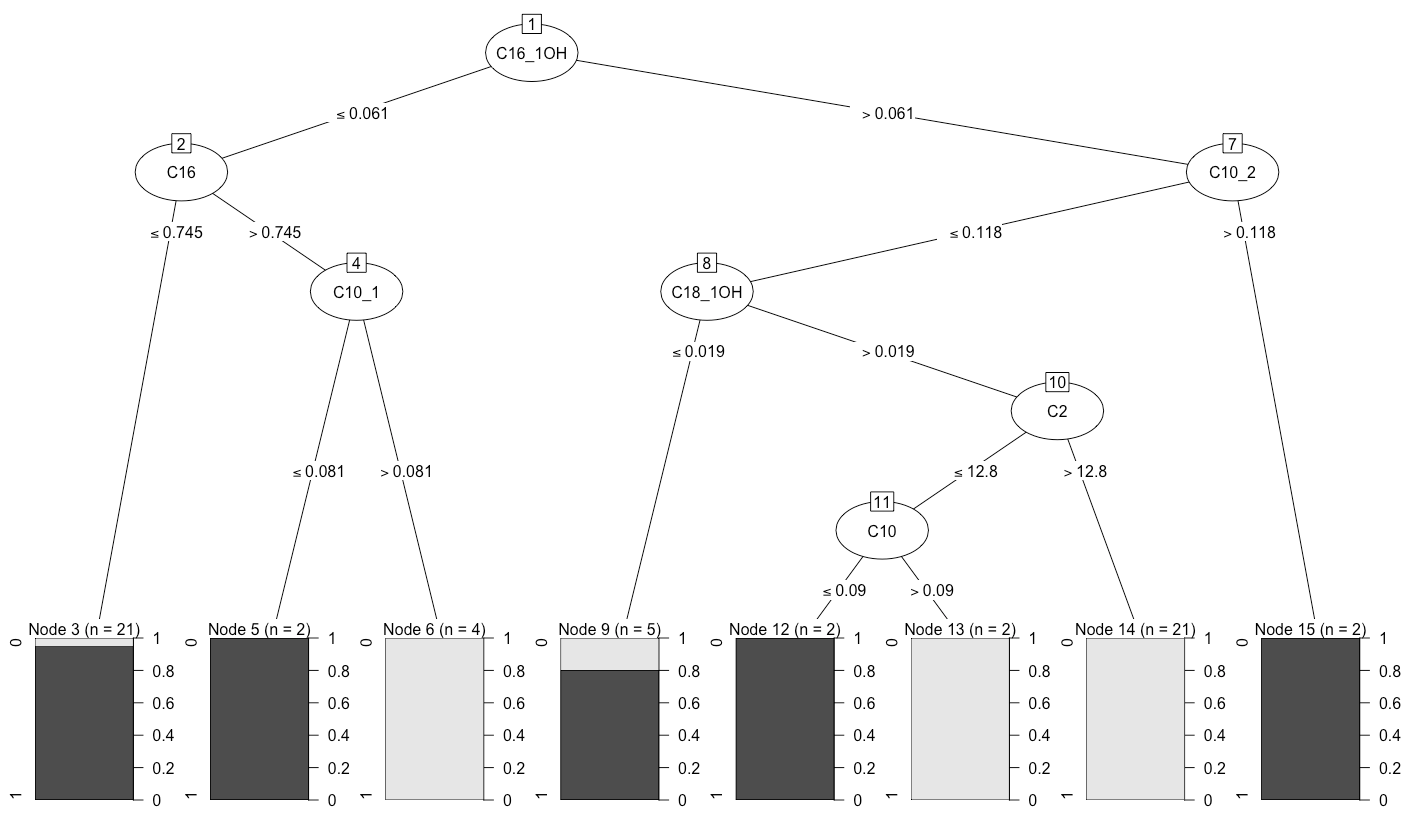
\includegraphics[width=12cm]{modc5}
\caption{Modelo propuesto por el algoritmo C5.0}
\label{fig:dm_c50}
\end{figure}


Para la comparaci�n de ambos modelos se utiliz� el an�lisis de �rea bajo la curva, la figura \ref{fig:auc_dm}, donde se demuestra que el modelo mostrado por el algoritmo C5.0 es superior.

\begin{figure}[H]
\centering
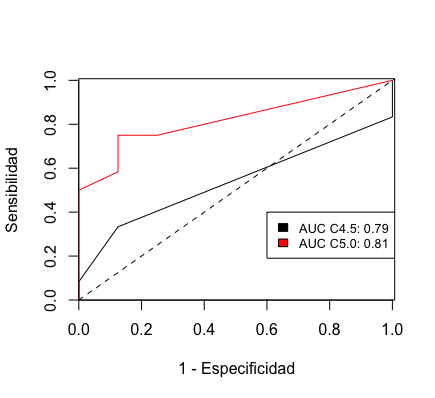
\includegraphics[width=10cm]{auc_mod_dm}
\caption{Comparaci�n de los resultados de los algoritmos C4.5 y C5.0 por AUC}
\label{fig:auc_dm}
\end{figure}

En la tabla \ref{tab:mod_c45_dm}  se muestra como el modelo propuesto por el algoritmo C4.5 se mantiene con adecuada sensibilidad, especificidad y respetable exactitud. En su validaci�n cruzada, continua teniendo una mayor sensibilidad que especificidad. En cuanto al desempe�o del algoritmo mediante validaci�n cruzada, se muestra el mismo resultado en la relaci�n sensibilidad y especificidad (tabla \ref{tab:al_c4.5}). \par
\newpage

\begin{table}[H]
\centering
\begin{tabular}{||c||c||}
\hline\hline
Estad�stico & Valor \\\hline \hline
Exactitud & 75\%\\
Sensibilidad & 88.8\%\\
Especificidad & 63.6\%\\
V. Predictivo Positivo & 66.6\%\\
V. Predictivo Negativo & 87.5\%\\\hline\hline
Validaci�n cruzada&\\\hline\hline
Exactitud  & 91.2\%  (IC 88.4\%, 94\%)\\
Sensibilidad & 91.6\% (IC 88.6\%, 94.6\%)\\
Especificidad & 90\% (IC 86.5\%, 93.4\%)\\
V. Predictivo Positivo & 94.1\% (IC 92.1\%, 96.2\%)\\
V. Predictivo Negativo &  90.8\% (IC 86.9\%, 94.7\%)\\
%AUC & 89.6 \% (IC 88.1\%,  891.1\%)\\
\hline\hline
\end{tabular}
\caption{Desempe�o del modelo propuesto por el Algoritmo C4.5}
\label{tab:mod_c45_dm}
\end{table}



\begin{table}[H]
\centering
\begin{tabular}{||c||c||}
\hline\hline
Estad�stico & Valor \\\hline \hline
Exactitud  & 66\%  (IC 63.1\%, 68.9\%)\\
Sensibilidad & 75\% (IC 71.2\%, 78.7\%)\\
Especificidad & 61.5\% (IC 56.6\%, 66.3\%)\\
V. Predictivo Positivo & 71.1\% (IC 67\%, 75.2\%)\\
V. Predictivo Negativo &  68\% (IC 63.8\%, 73.7\%)\\
%AUC & 63.5\% (IC 60.7\%,66.2\%)\\
\hline\hline
\end{tabular}
\caption{Desempe�o del Algoritmo C4.5 en validaci�n cruzada}
\label{tab:al_c4.5}
\end{table}

% De aqui en adelante es C5.0
En la tabla \ref{tab:c50}  , correspondiente al desempe�o del modelo dado por el algoritmo c5.0 se observa como pierde algo de exactitud, sin embargo,  se mantiene competitivo en cuanto a sensibilidad no as� en el valor predictivo positivo y negativo. En la validaci�n cruzada del modelo, se mantiene con adecuado VPP y VPN. 

\begin{table}[H]
\centering
\begin{tabular}{||c||c||}
\hline\hline
Estad�stico & Valor \\\hline \hline
Exactitud & 70\%\\
Sensibilidad & 87.5\%\\
Especificidad & 58.3\%\\
V. Predictivo Positivo & 58.3\%\\
V. Predictivo Negativo & 87.5\%\\\hline\hline
Validaci�n cruzada&\\\hline\hline
Exactitud  & 90.2\%  (IC 83.1\%, 97.4\%)\\
Sensibilidad & 90.7\% (IC 80.9\%, 100\%)\\
Especificidad & 92.7\% (IC 87\%, 98.4\%)\\
V. Predictivo Positivo & 91.2\% (IC 84.2\%, 98.3\%)\\
V. Predictivo Negativo &  91.1\% (IC 80.5\%, 100\%)\\
\hline\hline
\end{tabular}
\caption{Desempe�o del modelo propuesto por el Algoritmo C5.0}
\label{tab:c50}
\end{table}

En la validaci�n cruzada, tabla \ref{tab:c50_1} se mantiene competitivo con respecto al algoritmo algoritmo c4.5, con excepci�n de la AUC donde el c5.0 es mayor, (figura \ref{fig:algos_dm}).


\begin{table}[h]
\centering
\begin{tabular}{||c||c||}
\hline\hline
Validaci�n cruzada&\\\hline\hline
Exactitud  & 69.4\%  (IC 57.1\%, 81.7\%)\\
Sensibilidad & 72.2\% (IC 57.8\%, 86.5\%)\\
Especificidad & 69.8\% (IC 49.8\%, 89.8\%)\\
V. Predictivo Positivo & 77.3\% (IC 61.9\%, 92.8\%)\\
V. Predictivo Negativo &  67.4\% (IC 47.4\%, 87.3\%)\\
\hline\hline
\end{tabular}
\caption{Desempe�o del algoritmo C5.0 en validaci�n cruzada}
\label{tab:c50_1}
\end{table}

\newpage
\begin{figure}[H]
\centering
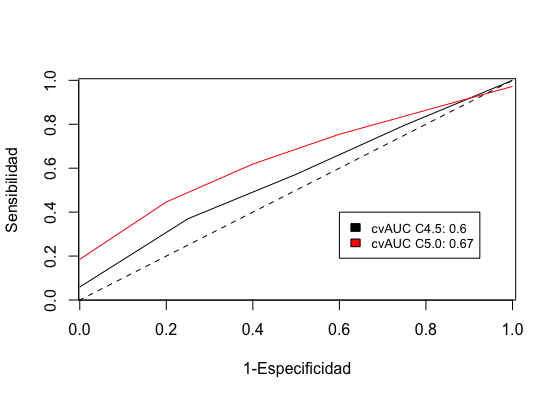
\includegraphics[width=10cm]{algos_auc_dm}
\caption{Validaci�n cruzada de AUC de algoritmo C5.0}
\label{fig:algos_dm}
\end{figure}

\subsection{Selecci�n de variables previamente realizado mediante regresi�n log�stica}

En las tablas \ref{tab:cf4.5} y \ref{tab:cf50}, siguientes se puede observar que utilizar una reducci�n de dimensiones mediante la regresi�n log�stica con pasos adelante (FS/LR) empeora el desempe�o de ambos algoritmos, el algoritmo con mejor desempe�o global es el C4.5. En la figura \ref{fig:auc_fs_dm}  se muestra el AUC  para ambos modelos.

\begin{table}[h]
\centering
\begin{tabular}{||c||c||}
\hline\hline
Estad�stico & Valor\\\hline\hline
Exactitud  & 55\%  \\
Sensibilidad & 33.3\% \\
Especificidad & 87.5\% \\
V. Predictivo Positivo & 80\% \\
V. Predictivo Negativo &  46\% \\  \hline \hline
Vallidaci�n cruzada & \\ \hline \hline
Exactitud & 81\% (IC 69.2\%, 94.6\%)\\
Sensibilidad & 72.5\% (IC 56.3\%, 88.6\%)\\
Especificidad & 90\% (IC 79\%, 100\%)\\
V. Predictivo Positivo & 91.6\% (IC 82.2\%, 100\%)\\
V. Predictivo Negativo & 78.9\% (63.9\%, 93.8\%)\\
\hline\hline
\end{tabular}
\caption{Desempe�o del modelo C4.5 con FS/LR}
\label{tab:cf4.5}
\end{table}
%%%% sigue con c5.0 fslr

\begin{table}[h]
\centering
\begin{tabular}{||c||c||}
\hline\hline
Estad�stico & Valor\\\hline\hline
Exactitud  & 50\%  \\
Sensibilidad & 25\% \\
Especificidad & 87.5\% \\
V. Predictivo Positivo & 75\% \\
V. Predictivo Negativo &  43.7\% \\  \hline \hline
Vallidaci�n cruzada & \\ \hline \hline%
Exactitud & 69.4\% (IC 59\%, 79.8\%)\\
Sensibilidad & 72.2\% (IC 60\%, 84.3\%)\\
Especificidad & 69.8\% (IC 52.8\%, 86.7\%)\\
V. Predictivo Positivo & 77.3\% (IC 64.2\%, 90.4\%)\\
V. Predictivo Negativo & 67.4\% (50.5\%, 84.2\%)\\
\hline\hline
\end{tabular}
\caption{Desempe�o del modelo C5.0 con FS/LR}
\label{tab:cf50}
\end{table}


\begin{figure}[H]
\centering
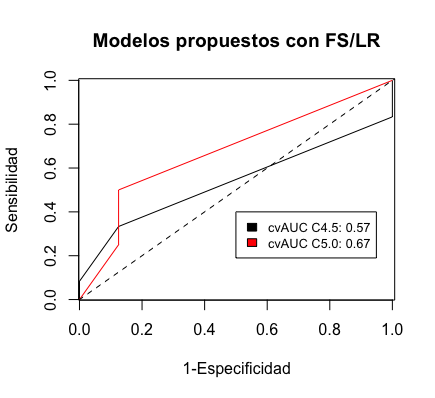
\includegraphics[width=10cm]{auc_modfs_dm}
\caption{AUC de modelos dados con reducci�n de dimensiones con FS/LR} 
\label{fig:auc_fs_dm}
\end{figure}
\vspace{-1cm}


\subsection{Evaluaci�n del desempe�o mediante bootstrap}



En esta secci�n se muestra el desempe�o de los algoritmos mediante un remuestreo bootstrap de los datos de entrenamiento. Este remuestreo se realiz� 1000 veces y se obtuvo la media y el intervalo de confianza para cada variable.

En la figura \ref{fig:b_dm} se observa claramente que el algoritmo con mayor �rea bajo la curva fue el que reuni� el C5.0 FS/LR, adem�s presento una de las mayores especificidades, aunque todos los algoritmos tienden a tener resultados muy similares.
\vspace{3cm}
\begin{figure}[H]
\centering
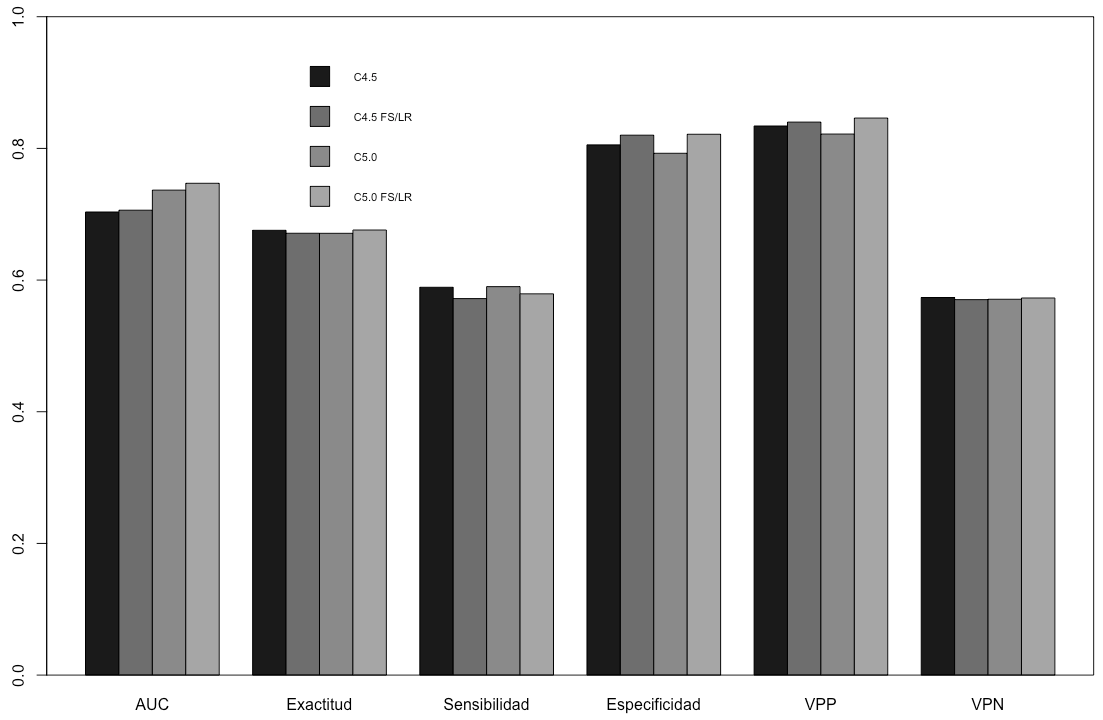
\includegraphics[width=10cm]{b_diabetes}
\caption{Desempe�o de los algoritmos mediante bootstrap}
\label{fig:b_dm}
\end{figure}

\subsection{�rbol de decisi�n costo sensible}

Se puede observar como en la tabla \ref{tab:dm_costo} se puede obtener una mejor exactitud al darle un peso distinto al 0.5. El mejor �rbol fue al que se le dio 0.67  con Estimado DM / Actual = Normal), con una exactitud del 84.6\%. \vspace{1cm}

\begin{table}[h]
\centering
\begin{tabular}{|c|c|c|}\hline
\begin{minipage}{.33\textwidth}
Costo (Estimado = DM/ \\Actual = Normal) 
\end{minipage}
& \begin{minipage}{0.33\textwidth}
 Costo (Estimado = Normal/\\Actual = DM) 
 \end{minipage}
 & Exactitud\\\hline
0.25 & 0.75 & 81.3  \\\hline
0.75 & 0.25 & 84.8  \\\hline
0.33 & 0.67 & 83.5  \\\hline
0.67 & 0.33 &  84  \\\hline
0.5 & 0.5 &  81 \\\hline
\end{tabular}
\caption{Resultados de clasificaci�n de DM con diferentes costos}
\label{tab:dm_costo}
\end{table}
\newpage

\section{Look Ahead Decision Tree.}

En la tabla \ref{tab:dm_look}, se puede observar que este algoritmo no es eficiente para clasificar a los pacientes con diabetes, ya que se mantiene con una exactitud muy cercana o inferior al 50\%. Esto con diferentes Deep y parametros B para su ajuste.

\begin{table}[h]
\centering
\begin{tabular}{|c|c|c|c|}\hline
                  & Deep 1 & Deep 2 & Deep 3 \\ \hline
B = 0.01 &  45.5 &  53.0 & 53.2   \\\hline
B = 0.03 &  45.5& 53.2 & 45.7  \\\hline
B= 0.06 & 53.3  &52.8  & 38.9  \\\hline
B = 0.09 & 53.2 &  53.0& 45.8  \\\hline
B = 0.1&  43.7  &  53.3 & 53.2 \\\hline
\end{tabular}
\caption{Resultados para clasificar pacientes con Diabetes Mellitus con diferente beta (B) y diferente profundidad  (Deep) de vista hacia adelante.}
\label{tab:dm_look}
\end{table}


\subsection{Meta caracter�sticas}

Esta dificultad en la clasificaci�n de diabetes mellitus, se demuestra de nueva cuenta en la tabla \ref{tab:meta_dm}, donde se muestra que los algoritmos C4.5 y C5.0 mejoran ligeramente la exactitud de clasificaci�n, sin embargo no alcanzan el 80\% de exactitud. La mejor exactitud la tuvo el algoritmo C5.0 con los datos originados de la Multiplicaci�n de variables sin los datos crudos.


\begin{table}[h]
\centering
\begin{tabular}{|c|c|c|}\hline
 				& C4.5 & C5.0  \\\hline
Suma &  56.9  &  72.2      \\\hline
Suma + & 56.9   &   73.5     \\\hline
Resta & 60.7  &    73.5   \\\hline
Resta + &   62.0  &  68.8        \\\hline
Multiplicaci�n &  63.2  &    74.7    \\\hline
Multiplicaci�n + & 64.5   &   71     \\\hline
\end{tabular}
\caption{Exactitud (\%) de los algoritmos con metacaracteristicas en Diabetes mellitus}
\label{tab:meta_dm}
\end{table}

En este caso de clasificar pacientes con diabetes mellitus agregando las meta caracter�sticas, mediante el algoritmo costo sensible, se puede ver en la tabla \ref{tab:csdt_metadm} que no se mejora la exactitud, siendo muy parecido en exactitud el que da un costo (25 - 75) y las meta caracter�sticas originadas por multiplicaci�n (las originadas con la resta tambi�n tienen una exactitud del 84.1\%). 


\begin{table}[h]
\centering
\begin{tabular}{|c|c|c|c|c|c|}\hline
 	Costos	& 0.25 - 0.75 & 0.75 - 0.25 & 0.33 - 0.67 & 0.67 - 0.33 & 0.5 - 0.5   \\\hline
Suma & 77.2  & 86   &  77.6 & 81 &  75.9  \\\hline
Suma + & 83.2   & 84.8   &76.7  & 80.5 &  82.9   \\\hline
Resta & 78.4	&  80.6 & 82.6 & 81 &  84.1   \\\hline
Resta + &  78.4 &  84.4   & 79.3 & 79.3  &  81.6    \\\hline
Multiplicaci�n & 84.1 &  76.5   &  81.4&  78.8 &  83.5  \\\hline
Multiplicaci�n + & 79.1  &  82.2 & 80.6 & 83.5 & 77.8   \\\hline
\end{tabular}
\caption{Exactitud (\%) de los algoritmos con metacaracteristicas con CSDT en Diabetes Mellitus}
\label{tab:csdt_metadm}
\end{table}


El algoritmo look ahead no mejora la clasificaci�n a�n con las meta caracter�sticas (tabla \ref{tab:metalook_dm}).

\begin{table}[h]
\centering
\begin{tabular}{|c|c|c|c|}\hline
                  & Deep 1 & Deep 2 & Deep 3 \\ \hline
Suma &  45.8  &  45.5  &  52.8 \\\hline
Suma + & 53.2  &   52.8 &   45.5   \\\hline
Resta & 65.7 & 64.4   &  66.7     \\\hline
Resta + &  63 &  63.5  & 63.2  \\\hline
Multiplicaci�n &  45.5  &   53.2   &  53   \\\hline
Multiplicaci�n + &  53.3  &   53.2 & 53.3  \\\hline
\end{tabular}
\caption{Exactitud (\%) de los algoritmos con metacaracteristicas con LADT previa selecci�n de variables en Diabetes Mellitus (todos fueron con B = 0.1)}
\label{tab:metalook_dm}
\end{table}


%
%
%
\section{Retinopat�a}

En esta secci�n se comentan los resultados de la aplicaci�n de los diferentes algoritmos para la clasificaci�n de pacientes con retinopat�a diab�tica.

\newpage

\subsection{Algoritmo C4.5 y C5.0}

En las figuras \ref{fig:retino_c45} y \ref{fig:retino_c50} , se muestran los modelos obtenidos por los algoritmos C4.5 y C5.0 en la predicci�n de retinopat�a diab�tica.

\begin{figure}[H]
\centering
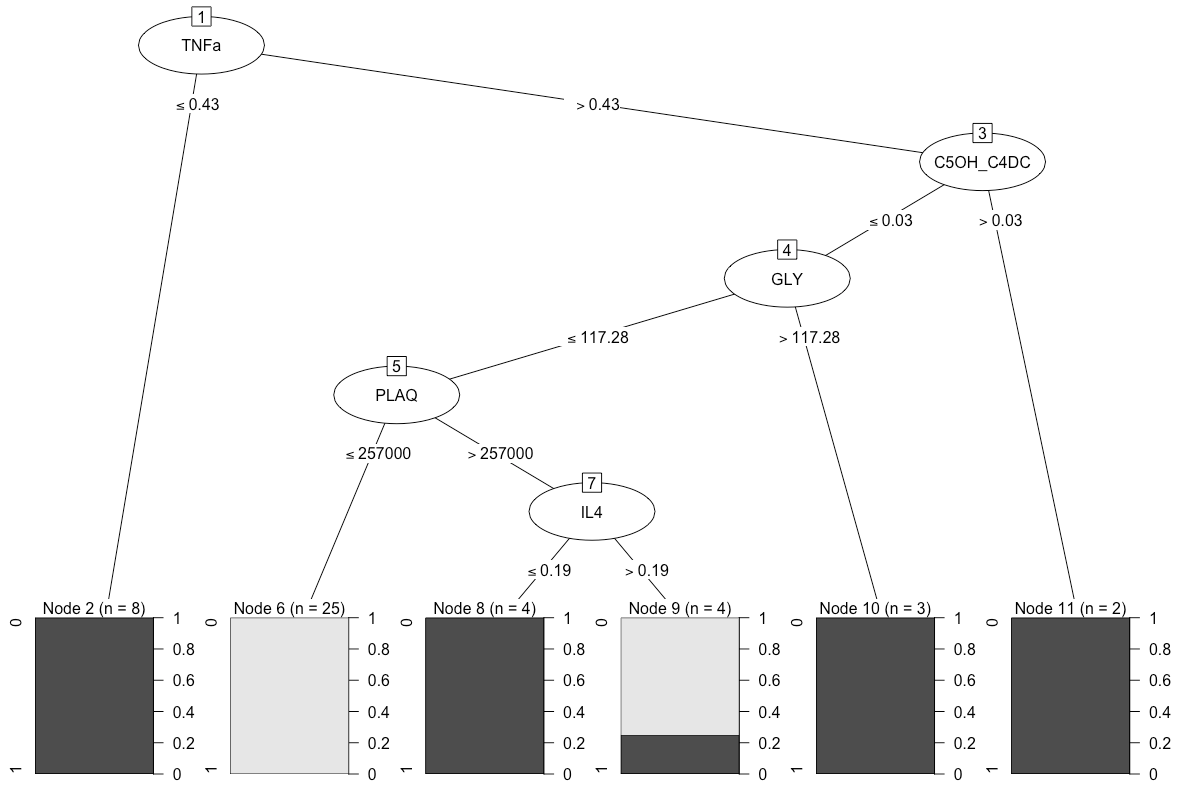
\includegraphics[width=10cm]{retino_c45}
\caption{Modelo obtenido por C4.5 para la clasificaci�n de retinopat�a diab�tica}
\label{fig:retino_c45}
\end{figure}


En este caso, se muestra (que como es de suponer por cuestiones biol�gicas) las variables obtenidas est�n relacionadas con un proceso inflamatorio (TNFa, IL4, plaquetas) y un proceso de alteraci�n metab�lica como es GLY (amino�cido, Glicina). En la tabla \ref{tab:retino_c45} se observa como al partir los datos (80\% de entrenamiento y 20\% de prueba) se tiene una alta sensibilidad pero con una exactitud no aceptable. Pudiendo sugerir que este modelo puede ser utilizado como escrutinio. Por otro lado, al realizarse una validaci�n cruzada 10 Folds se muestra un incremento en la exactitud y en el resto de par�metros de evaluaci�n del modelo.

\begin{table}[H]
\centering
\begin{tabular}{||c||c||}
\hline \hline
Estad�stico &  Valor \\\hline \hline
Exactitud & 50\%\\
Sensibilidad & 100\% \\
Especificidad & 45\% \\
V. Predictivo Positivo & 14.2\% \\
V. Predictivo Negativo & 100\% \\ \hline \hline
Validaci�n cruzada & \\ \hline \hline
Exactitud & 91\% (IC 79.3\%, 100\%)\\
Sensibilidad & 92.5\% (IC( 77.8\%, 100\%)\\
Especificidad & 96.8\% (IC 90.7\%, 100\%)\\
V. Predictivo Positivo & 95.8\% (IC 87.6\%, 100\%)\\
V. Predictivo Negativo & 90.6\% (IC 72.2\%, 100\%\\\hline \hline
\end{tabular}
\caption{Desempe�o de modelo C4.5}
\label{tab:retino_c45}
\end{table}


\begin{figure}[H]
\centering
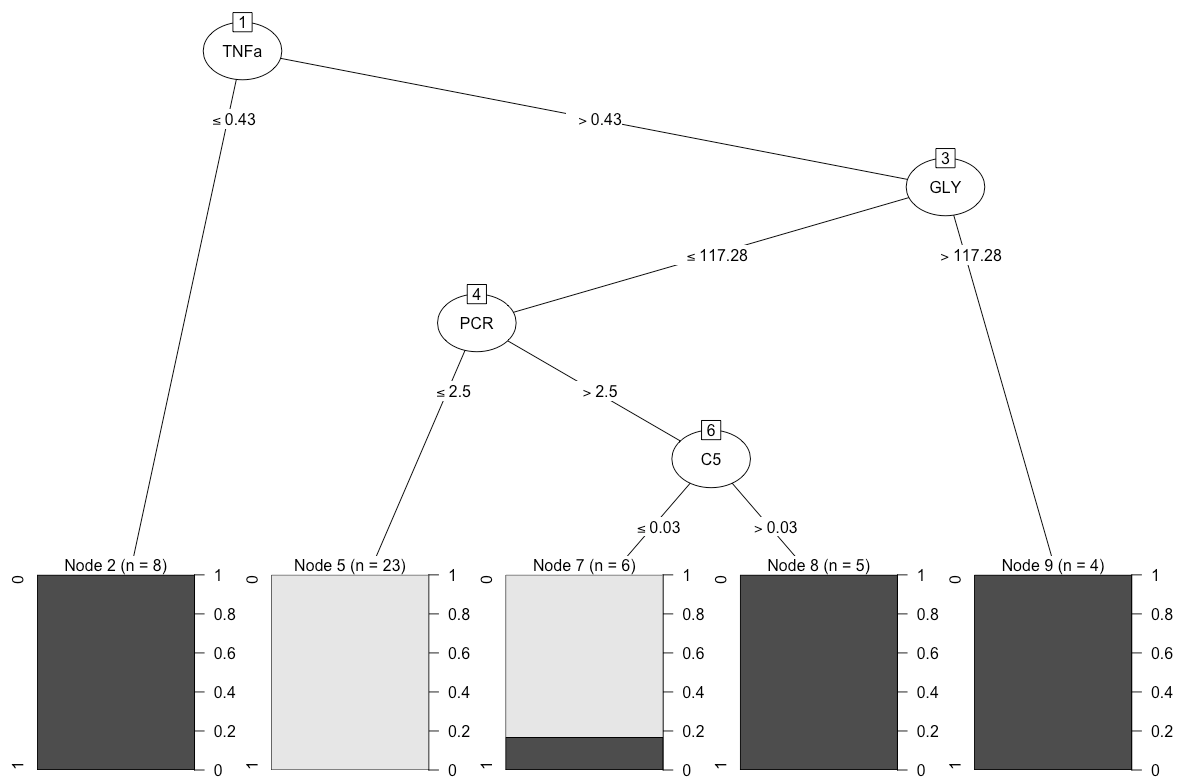
\includegraphics[width=12cm]{retino_c50}
\caption{Modelo obtenido por C5.0 para la clasificaci�n de retinopat�a diab�tica}
\label{fig:retino_c50}
\end{figure}
\newpage
El modelo C5.0 tambi�n incluye una acilcarnitina de cadena corta (relacionada a problemas metab�licos) pero no carboxilada. Este cambio puede ser debido al algoritmo que trata de producir �rboles de menor tama�o que su antecesor. As� tambi�n este algoritmo se mantiene con excelente sensibilidad, pero incrementa la exactitud y especificidad, tabla \ref{tab:c5.0_retino1}

\begin{table}[H]
\centering
\begin{tabular}{||c||c||}
\hline \hline
Estad�stico & Valor \\ \hline \hline
Exactitud & 75\%  \\
Sensibilidad & 100\% \\
Especificidad & 72.7\% \\
V. Predictivo Positivo & 25\% \\
V. Predictivo Negativo & 100\% \\ \hline \hline
Validaci�n cruzada & \\ \hline \hline
Exactitud & 97.9\%(IC 93.8\%, 100\%) \\
Sensibilidad & 93.7\% (IC 81.5\%, 100\%)\\
Especificidad & 100\% \\
V. Predictivo Positivo & 100\% \\
V. Predictivo Negativo & 97.5\% (IC 92.6\%, 100\%)\\ \hline \hline
\end{tabular}
\caption{Desempe�o de modelo obtenido del algoritmo C5.0}
\label{tab:c5.0_retino1}
\end{table}

\subsection{Selecci�n de variables previamente realizado mediante regresi�n log�stica}

En las tablas \ref{tab:frlr}, se puede observar que la selecci�n de variables mediante regresi�n log�stica no mejora la exactitud del modelo.
\newpage

\begin{table}[H]
\centering
\begin{tabular}{||c||c||}
\hline \hline
Estad�stico & Valor \\ \hline \hline
Exactitud & 58.3\% \\
Sensibilidad & 100\% \\
Especificidad & 54.5\% \\
V. Predictivo Positivo & 16.6\% \\
V. Predictivo Negativo & 100\% \\ \hline \hline
Validaci�n cruzada & \\ \hline \hline
Exactitud & 68.7\% (IC 64.1\%, 73.3\%)\\
Sensibilidad & 68.7\% (IC 57.5\%, 79.9\%)\\
Especificidad & 72.5\% (IC 67.1\%, 77.8\%)\\
V. Predictivo Positivo & 44.7\% (IC 35.2\%, 54.3\%)\\
V. Predictivo Negativo & 87.5\% (IC 83\%, 91.9\%)\\ \hline \hline
\end{tabular}
\caption{Exactitud de modelos C4.5 y C5.0, mediante regresi�n log�stica con paso hacia adelante.}
\label{tab:frlr}
\end{table}

\subsection{�rbol de decisi�n costo sensible}

En la tabla \ref{tab:costs_retino} se muestra como el algoritmo costo sensible puede mejorar la exactitud de la clasificaci�n mediante cualquier costo aplicado a la mala clasificaci�n de los sujetos. Llegando a tener una exactitud del 88.7\% en el modelo con el costo 0.25 - 0.75.

\begin{table}[h]
\centering
\begin{tabular}{|c|c|c|}\hline
\begin{minipage}{.33\textwidth}
Costo (Estimado = Retinopat�a/ \\Actual = Normal) 
\end{minipage}
& \begin{minipage}{0.33\textwidth}
 Costo (Estimado = Normal/\\Actual = Retinopat�a) 
 \end{minipage}
 & Exactitud\\\hline
0.25 & 0.75 &  88.7 \\\hline
0.75 & 0.25 &  87.9 \\\hline
0.33 & 0.67 &  89 \\\hline
0.67 & 0.33 &   84.5 \\\hline
0.5 & 0.5 &   84.4\\\hline
\end{tabular}
\caption{Resultados de clasificaci�n de Retinopat�a con diferentes costos}
\label{tab:costs_retino}
\end{table}


\section{Look Ahead Decision Tree.}

El �rbol de decisi�n obtenido por el algoritmo de Look Ahead, con diferentes Deep, puede incrementar ligeramente la exactitud, sobre todo con Deep 2 y par�metro Beta = 0.01, (tabla \ref{tab:deep_1}). Sin embargo no llega a ser tan competitivo como el �rbol obtenido con el modelo sensible a costo.

\begin{table}[H]
\centering
\begin{tabular}{|c|c|c|c|}\hline
                  & Deep 1 & Deep 2 & Deep 3 \\ \hline
B = 0.01 & 62.6  &  76.3 & 68.0 \\\hline
B = 0.03 & 69.6 & 66.3 & 76.6\\\hline
B= 0.06 & 71.0  & 76.0 & 68.6\\\hline
B = 0.09 & 67.6 & 72.3 & 68.6\\\hline
B = 0.1& 63.0   &  71.0 & 70.6\\\hline
\end{tabular}
\caption{Resultados para clasificar pacientes con Retinopat�a con diferente beta (B) y diferente profundidad  (Deep) de vista hacia adelante.}
\label{tab:deep_1}
\end{table}

\subsection{Meta caracter�sticas}

En esta secci�n se expondr�n los resultados de la aplicaci�n de los algoritmos en la base de datos creada mediante meta caracter�sticas.  En la tabla \ref{tab:meta_base} se puede observar que las meta caracter�sticas mejoran ligeramente la exactitud de la clasificaci�n. Sobre todo mediante el algoritmo C5.0 y con los datos obtenidos mediante multiplicaci�n con o sin los datos crudos.

\begin{table}[h]
\centering
\begin{tabular}{|c|c|c|}\hline
 				& C4.5 & C5.0  \\\hline
Suma & 58.6   &  73.6      \\\hline
Suma + & 58.6   &   73.3     \\\hline
Resta & 65.5   &   77.6    \\\hline
Resta + & 65.5    &   76       \\\hline
Multiplicaci�n &  72.4  &    82.3    \\\hline
Multiplicaci�n + &  72.4  &   82.3     \\\hline
\end{tabular}
\caption{Exactitud (\%) de los algoritmos con meta caracteristicas en Retinopatia}
\label{tab:meta_base}
\end{table}

En la tabla \ref{tab:meta_csdt}, se muestra como las meta caracter�sticas y el algoritmo costo sensible pueden incrementar la exactitud de la clasificaci�n de manera importante llegando a ser superior al 90\% como en los datos originados de la resta (90.9\%) y de la multiplicaci�n.


\begin{table}[H]
\centering
\begin{tabular}{|c|c|c|c|c|c|}\hline
 	Costos	& 0.25 - 0.75 & 0.75 - 0.25 & 0.33 - 0.67 & 0.67 - 0.33 & 0.5 - 0.5   \\\hline
Suma & 87.5  &  82.7  & 87.3  & 83.3 &  77.5  \\\hline
Suma + &  81.8  & 83.1   & 79.9 & 82.7 & 83.6    \\\hline
Resta & 83.6	&  90.9 & 85 &  86.7 &  85.3   \\\hline
Resta + & 87.5  & 89.2  & 87.9  &  86.2 & 86.2     \\\hline
Multiplicaci�n & 87.9 &  90   & 85 & 85.6  & 82.7   \\\hline
Multiplicaci�n + &  84 & 88.7  & 83.3 & 85.6  & 81.8   \\\hline
\end{tabular}
\caption{Exactitud (\%) de los algoritmos con meta caracter�sticas con CSDT en Retinopat�a}
\label{tab:meta_csdt}
\end{table}

El algoritmo de Look Ahead, incremento de manera ligera la exactitud del modelo. El �rbol con Depp 1 originado de los datos de Resta sin los datos crudos fue el que tuvo la mejor exactitud con 74.3\%. (Tabla \ref{tab:metaladt}).

\begin{table}[h]
\centering
\begin{tabular}{|c|c|c|c|}\hline
                  & Deep 1 & Deep 2 & Deep 3 \\ \hline
Suma & 67.3   &  67.3  &  66.6 \\\hline
Suma + &  66.6 & 66.6   &   67   \\\hline
Resta & 74.3 &  71.6  &   72.6    \\\hline
Resta + &  70.3 &  69.3  & 62.6  \\\hline
Multiplicaci�n &  67  &  67.3    &  67   \\\hline
Multiplicaci�n + &  67.3  &  67.6  & 67  \\\hline
\end{tabular}
\caption{Exactitud (\%) de los algoritmos con meta caracter�sticas con LADT previa selecci�n de variables en Retinopat�a (todos fueron con B = 0.1)}
\label{tab:metaladt}
\end{table}


\section{Software utilizado}

En esta tesis se utiliz� el paquete estad�stico R v 3.4.2 , Matlab 2016 y Weka v 3.8.2 . Las librer�as utilizadas en R son: pROC, DescTools, RWeka, caret, C50, corrplot, gbm, coin, psych, ROCR, OptimalCutpoints, RcmdrMisc, cvAUC.



\chapter{Contribuciones, conclusi�n y trabajo futuro}

\section{Contribuciones al an�lisis de datos}

El an�lisis de los datos utilizados en este trabajo, se caracterizan por ser de alta dimencionalidad y de gran dificultad de an�lisis. Los algoritmos base (por ejemplo C4.5 y C5.0) con los que se di� soluci�n al problema de clasificaci�n pueden ser mejorados con la previa selecci�n de variables con una regresi�n log�stica o con otras t�cnicas como el dar un paso hacia adelante en su algoritmo (Look Ahead) o con la propiedad de ser sensibles a costo. Las contribuciones se resumen puntualmente de la forma siguiente:

\subsection{GCSLADT supera otras variantes de �rbol de decisi�n y criterio de s�ndrome metab�lico para NAFLD}.

Dependiendo del problema a resolver se pueden utilizar las capacidades de este algoritmo para resolverlas, una de ellas la sensibilidad a costos cuando los datos son desbalanceados, en nuestro trabajo se presentaron dos casos as�: el conjunto de pacientes con h�gado graso no alcoh�lico y el sub grupo anidado de pacientes con retinopat�a. De estos los datos con mayor desbalance fue la de NAFLD y  el algoritmo present� una exactitud que rondaba el 92\%. \par

En el caso del uso del paso hacia adelante (Look Ahead), se demuestra que se debe tener en consideraci�n que la cantidad de pasos hacia adelante. Ya que el dar muchos pasos hacia adelante pudieran alterar la clasificaci�n final del algoritmo (efecto del horizonte). Tambi�n que este efecto pudiera ser alterado por el criterio de parada (beta) en la partici�n del �rbol.\par

\subsection{Active, Online, reinforcement e incremental learning pueden ser incorporados en la estructura del algoritmo GCSLADT.}

Algoritmos como Active, Online, Reinforcement e Incremental Learning pueden ser incorporados al algoritmo base de GCSLADT. Con la intenci�n de incrementar el desempe�o del algoritmo inicial. Se hace hincapi� a considerar el tipo de problema albergado en los datos as� como el tama�o de los mismos para la decisi�n de usar tal o cual aprendizaje.

\subsection{Incorporaci�n de meta caracter�sticas ayuda a dar mayor exactitud de �rbol de decisi�n para clasificar complicaciones del s�ndrome metab�lico.}

Las meta caracter�sticas que se utilizaron en este trabajo incluyeron las opraciones algebraicas de de suma, resta y multiplicaci�n.  Mostraron la capacidad de incrementar la exactitud en la predicci�n de las complicaciones del s�ndrome metab�lico.  Esta exactitud es incrementada todav�a mas al agregar un ``peso'' a las desiciones equivocadas (Sensible a costo) del algoritmo, sobre todo para datos desbalanceados (ej. H�gado graso no alcoh�lico).


\subsection{Las t�cnicas de elegir caracter�sticas (NCA,FA, Forward selection) reduce la complejidad computacional del �rbol de decisi�n por disminuir la dimensi�n sin reducir la exactitud.}

La selecci�n de variables es un paso muy importante con la alta dimensionalidad de los datos. Adem�s algoritmos como look ahead que mejoran la exactitud de los algoritmos tradicionales, tienen un limite de dimensiones (100 variables en caso de Look Ahead) haciendo muy necesario este paso.

Por otro lado,  el escoger las variables mas importantes sin perdida de desempe�o del algoritmo disminuye el costo computacional de la clasificaci�n.

\section{Contribuciones a la literatura m�dica}

En la literatura medica, existen multiples intentos (los cuales fueron revisados en esta tesis) de clasificar adecuadamente pacientes sanos y con h�gado graso no alcoh�lico; adem�s en este mismo trabajo se realiz� un �rbol de decisi�n hecho por el experto, con los criterios de clasificaci�n de s�ndrome metab�lico, demostrando la necesidad de un algoritmo inteligente.
En el uso de algoritmos como C4.5 y C5.0 se pudo demostrar que se puede mejorar la clasificaci�n de pacientes con h�gado graso no alcoh�lico mediante la combinaci�n de variables qu�micas, cl�nicas y metabol�micas.\par

Se demostr� como las alteraciones en las acilcarnitinas (principalmente de cadena larga, como C16\_OH), est�n relacionadas con la presencia de h�gado graso. El incremento en los niveles de las acilcarnitinas es asociado a esta enfermedad hep�tica y resistencia a la insulina. Esto ultimo dado a que la carnitina C16\_1OH (y tambi�n otras como la C14\_1, C18\_1OH) son unas de las principales variables que pueden clasificar a los pacientes con diabetes mellitus tipo 2.\par

En este mismo sentido, en este trabajo se documenta por primera vez la utilidad de las acilcarnitinas (como �nicas variables) para clasificar al paciente con diabetes. Por otro lado, tambi�n se logra confirmar la relaci�n entre el trastorno metab�lico expresado en estas variables metabol�micas y la presencia de retinopat�a. Aunque pareciera aventurado confirmar en este momento, pero parece ser que hay bases suficientes para sostener la teor�a de la retinopat�a del paciente obeso.\par

Por otro lado, el tipo de an�lisis llevado a cabo originar nuevas hip�tesis. El poder fundamentar que la clasificaci�n de retinopat�a por acilcarnitinas es posible, nos sugiere la realizaci�n de estudios dise�ados para evaluar causalidad.

\section{Conclusiones}

Las conclusiones de este trabajo son resumidas a continuaci�n:

\begin{itemize}
\item Desarrollamos �rbol de Decisi�n Sensible a Costos y con Mirada Adelante Generalizado (Generalized Cost Sensitive Look Ahead Decision Tree , GCSLADT) para automatizar el diagnostico de las complicaciones del s�ndrome metab�lico.
\item Demostramos el poder de meta caracter�sticas para clasificar las complicaciones del s�ndrome metab�lico.
\item Utilizamos decision tree para clasificar las complicaciones del s�ndrome metab�lico por su interpretabilidad por los m�dicos.
\item Comparamos el rendimiento de �rbol de decisi�n con diferentes scores diagn�sticos publicados en la literatura.
\item El perfil bioqu�mico es suficiente para clasificar NAFLD con �rbol de decisi�n autom�ticamente.
\end{itemize}


\section{Trabajo futuro}

Actualmente existe mucho trabajo futuro por realizar, de entre ellos se remarcan los siguientes:
El algoritmo de �rboles de decisi�n utiliza el criterio de reducci�n de entrop�a para la partici�n de los datos.
\begin{itemize}
\item  Generalized Cost Sensitive Look Ahead Decision Tree (GCSLADT) funciona mejor para clasificar NAFLD, presencia de diabetes y Retinopat�a, se probara en otras enfermedades.
\item Queremos  investigar el agregar diferentes tipos de aprendizaje (Any time, High speed, ensamble) a la estructura de GCSLADT. 
\end{itemize}



%\chapter{Conclusi�n y trabajo futuro}

\section{Conclusiones}

Las conclusiones de este trabajo son resumidas en la siguiente lista:

\begin{itemize}
\item Desarrollamos �rbol de Decisi�n Sensible a Costos y con Mirada Adelante Generalizado (Generalized Cost Sensitive Look Ahead Decision Tree , GCSLADT) para automatizar el diagnostico de las complicaciones del s�ndrome metab�lico.
\item Demostramos el poder de meta caracter�sticas para clasificar las complicaciones del s�ndrome metab�lico.
\item Utilizamos decision tree para clasificar las complicaciones del s�ndrome metab�lico por su interpretabilidad por los m�dicos.
\item Comparamos el rendimiento de �rbol de decisi�n con diferentes scores diagn�sticos publicados en la literatura.
\item El perfil bioqu�mico es suficiente para clasificar NAFLD con �rbol de decisi�n autom�ticamente.
\end{itemize}


\section{Trabajo futuro}

Actualmente existe mucho trabajo futuro por realizar, de entre ellos se remarcan los siguientes:
El algoritmo de �rboles de decisi�n utiliza el criterio de reducci�n de entrop�a para la partici�n de los datos. Existen otros como el Gini Index y el   voy a considerar la varianza de la clase.
\begin{itemize}
\item  Generalized Cost Sensitive Look Ahead Decision Tree (GCSLADT) funciona mejor para clasificar NAFLD, presencia de diabetes y Retinopat�a, se probara en otras enfermedades.
\item Queremos  investigar el agregar diferentes tipos de aprendizaje (Any time, High speed, ensamble) a la estructura de GCSLADT. 
\end{itemize}


 

\bibliography{nafld}

\setcounter{secnumdepth}{-1} % no level is numbered

\chapter{Anexo}

\section{Regresi�n log�stica.}

Los m�todos de regresi�n se han convertido en una parte principal del an�lisis de los datos, en lo que se refiere a la relaci�n entre las variables respuesta y las explicativas. Se puede distinguir la regresi�n log�stica de los otros tipos de regresi�n, porque la variable respuesta es binaria o dicot�mica. Donde la variable respuesta debe ser predicha mediante una probabilidad, y no mediante la predicci�n de un valor determinado continuo .  

Se puede usar la cantidad $\pi(x) = E(Y|x)$ para representar la media condicional de Y dado x cuando la regresi�n log�stica es usada. La ecuaci�n especifica a este modelo es:

\begin{equation}
\pi(x) = \frac{e^{\beta_0 + \beta_1 x}}{1+ e^{\beta_0 + \beta_1 x}}
\end{equation}

$\pi(x)$ se puede transformar en la transformaci�n logit:

\begin{equation}
g(x) = ln[ \frac{\pi(x)}{1 - \pi(x)}]
= \beta_0 + \beta_1 x
\end{equation}

La importancia de esta transformaci�n es que g(x) tiene propiedades deseables de un modelo de regresi�n lineal. El logit, g(x), es lineal en sus par�metros, puede ser continuo y su rango de $- \infty$ a $+\infty$ dependiendo del rango de x.

La cantidad de variables incluidas en el modelo deben ser k-1 variables, siendo K la cantidad de observaciones a predecir.  Por lo que se debe tener cuidado al momento de incluir las variables y no saturar el modelo. 

La selecci�n paso a paso es ampliamente usado en otros tipos de regresiones como en la lineal. Este procedimiento se basa en la selecci�n estad�stica de las variables "mas importantes" y esta importancia es medida mediante la significancia estad�stica de los coeficientes de las variables. En la regresi�n log�stica se utiliza el mayor cambio de log verosimilitud en relaci�n con un modelo que no contiene la variable.

La selecci�n de variables hacia adelante  (\textbf{Forward},en ingl�s), es uno de los tres m�todos disponibles para la selecci�n autom�tica de variables (los otros son, hacia atras (\textbf{backward}) y exhaustivo (\textbf{exhaustive}).  Estos m�todos pueden ser criticados por reunir variables que cl�nicamente pudieran ser retiradas del modelo y se sugiere siempre agregar variables por expertise del investigador. Sin embargo, en el presente trabajo se utiliza este m�todo ya que en la actualidad no se cuenta con una manera cl�nica de selecci�n de variables.

A continuaci�n se describe el algoritmo de selecci�n hacia adelante.

\begin{enumerate}
	\item Paso (0): Inicia con el ajuste del "modelo solo con intercepto" y la evaluaci�n de su log-verosimilitud. Esto es seguido de el ajuste de cada posible variable mediante regresiones log�sticas univariadas. Se agregan solo las variables con menor "p valor".
	\item Paso (1):  Se comienza con el ajuste de la regresi�n log�stica, conteniendo ya la primera variable. Se ajusta el siguiente modelo agregando la variable con menor "p valor", y se procede a realizar el paso 2, de otra forma se detiene.
	\item Paso (2): Se ajusta el modelo conteniendo las dos primeras variables. Dado que la primera variable agregada puede no ser ya significativa (en presencia de la segunda variable), se realiza una eliminaci�n hacia atr�s. Esto basado en el cambio en el p valor con o sin la primera variable.
	\item Paso (3): El paso (3) es id�ntico al paso (2). El programa ajusta el modelo que incluye la variable seleccionada durante el paso previo. Este paso continua hasta el paso (s).
	\item Paso (S): Este paso, ocurre cuando:
		\begin{enumerate}
			\item Todas las variables an entrado al modelo �
			\item Todas las variables en el modelo tienen p valor, para remover las que tengan menor p valor.
		\end{enumerate}

\end{enumerate}

\section{Bootstrap}

El ``bootstrap'' es una de las t�cnicas que ahora es parte de un abanico de pruebas estad�sticas no parametricas que comunmente son llamados m�todos de remuestreo. Fue definido por Efron en el a�o 1979  como un procedimiento de remuestreo. El objetivo del bootstrap es estimar un par�metro de los dato (media, mediana o desviaci�n est�ndar). Tambi�n se pueden construir intervalos de confianza \cite{chernick2014introduction}.

El elemento b�sico para el boostraping es la distribuci�n empirica. Esta distribuci�n empirica es solo la distribuci�n discreta que da igual peso a cada punto (�sea probabilidad 1/n). El principio del bootstrap menciona que F es la distribuci�n de la poblaci�n, y T(F) es la funci�n que define el par�metro a obtener. Nosotros deseamos estimar un par�metro cualquiera de una muestra de $n$ observaciones independientes e igualmente distribuidas. Entonces $F_n$ juega el papel de F y $F_n *$ la distribuci�n bootstrap, tiene el papel $F_n *$ en el proceso de remuestreo.

De esta forma nosotros calculamos la media del par�metro con el que se eval�a el modelo (ej. sensibilidad, especificidad, etc.).


\newpage
\section{Pseudoc�digo ID3}

En el siguiente espacio se describir� el pseudoc�digo de ID3

\begin{algorithm}
\SetKwInOut{Create}{Create}
\SetKwBlock{Otherwise}{Otherwise}{end}
ID3 (\textbf{Ejemplos}, \textbf{Atributo}, \textbf{Atributos})
\Create{Un nodo ra�z para el �rbol; asigna todos los \textit{Ejemplos} a la ra�z}
\If{ Todos los \textbf{Ejemplos} son positivos}{\Return un solo nodo ra�z, con etiqueta $=+$}
\If{ Todos los \textbf{Ejemplos} son negativos}{\Return un solo nodo ra�z, con etiqueta $=-$}
\If{ Los \textbf{Atributos} est�n vacios}{\Return un solo nodo ra�z, con la etiqueta =  el valor mas com�n de \textbf{Atributo} en \textbf{Ejemplos}}
\Otherwise{A $\leftarrow$ el atributo de \textbf{Atributos} que mejor clasifica en \textbf{Ejemplos}\\
El atributo decisi�n para la ra�z $\leftarrow$ A\\
\ForEach{Posible valor $v_i$ de A}{Agregar una nueva rama debajo de la ra�z, correspondiente a la prueba $A = v_i$\\Haz que $\text{Ejemplos}_vi$ sea el subgrupo de \textbf{Ejemplos} que tienen el valor $vi$ para $A$\\
\If (Esta vac�o){$\text{Ejemplos}_{vi}$}{Debajo de esta nueva rama se agrega un nodo hoja con etiqueta = el valor mas com�n de \textbf{Atributo} en \textbf{Ejemplos}\\ \Else{Debajo esta nueva rama agregar el sub �rbol\\
ID3(\textbf{Ejemplos}, \textbf{Atributo}, \textbf{Atributos}\{A\})}} }
\Return ra�z}
% viene den el archivo id3 pseudocode
\end{algorithm}
\newpage

\section{Pseudoc�digo C4.5}
Se presenta el pseudoc�digo del algoritmo C4.5.


\begin{algorithm}
\SetKwInOut{Input}{Input}
\SetKwInOut{Output}{Output}
\SetKwFor{ForEach}{foreach}{do}{end}
\SetKwRepeat{Repeat}{repeat}{until}
\Input{ atributos valuados en el conjunto de datos D}
�rbol = \{\}\\
\If{ D es ``puro'' u otro criterio de paro se cumple}{termina}
\ForAll{Atributos $\in$D}{Computar el criterio de informaci�n te�rico si particionamos en a}
$a_{\text{mejor}}$ = El mejor atributo acorde a los criterios computados antes.\\
$D_{v}$ = Inducci�n de los sub-datos de $D$ basados en $a_{\text{best}}$\\
\ForAll{$D_{v}$}  {$\text{�rbol}_{v} = C4.5(D_v)$ Adjunta el $\text{�rbol}_{v}$ a la rama correspondiente del �rbol}
\Return{�rbol}
\caption{Pseudoc�digo de algoritmo C4.5}
\end{algorithm}

\section{Pseudoc�digo del boosting C5.0}

Para describir el desarrollo de este algoritmo, asumiremos que el conjunto de muestras $S$ consiste de $n$ muestras y un sistema de aprendizaje que construye diferentes �rboles de decisi�n. El boosting construye  �rboles de decisi�n de las muestras, esto es, construye $T$ �rboles de decisi�n, y $C^t$ es el �rbol de decisi�n arrojado por el sistema de aprendizaje en el intento $t$ y $C^*$ es el �rbol final que es formada al agregar los $T$ �rboles de decisi�n. $w_{i}^{t}$ es el peso de la i-�sima muestra en la prueba $t$ ($i = 1,2,\dots, N; t= 1,2, \dots,T$). $P_{i}^t$ es el factor normalizado de $w_{i}^t$ y $\beta_t$  es el factor que ajusta el peso. Tambi�n se puede definir una funci�n indicadora:

\begin{equation}
\theta^t (i) =
\begin{cases}
1 \text{, la i-�sima muestra es mal clasificada}\\
0 \text{, la i-�sima muestra es bien clasificada}
\end{cases}
\end{equation}

Los principales pasos para el boosting es el siguiente:

\begin{enumerate}
	\item Inicializar las variables; ajusta un valor al numero de $T$ (usualmente es 10). Ajusta $t = 1,w_{i}^1 = \frac{1}{n}$.
	\item Calcula $P_{i}^t = w_{i}^t / \sum^{n}_{i=0} (w_{i}^{t}$, donde $\sum^{n}_{i=0}(P_{i}^{y}) = 1$.
	\item Sea $P_{i}^t$ el peso de cada muestra y construye $C^t$ bajo esta distribuci�n.
	\item Calcula la taza de error de $C^t$ como $\epsilon^t = \sum_{i=0}^n (P_{i}^t \theta_{i}^t)$.
	\item Si $\epsilon^t <$ 0.5, los experimentos se terminan, sea $T = t +1$; de otra forma si $\epsilon^t =0$, los experimentos se terminan, sea $T = t$; de otra forma si $0 <\epsilon^t < 0.5$, ve al paso 6.
	\item Calcula $\beta^t = \epsilon^t/(1-\epsilon^t)$.
	\item Ajusta el peso acorde a la tasa de error, que es
	\[
	w_{i}^t{t+1} =
	\begin{cases}
	w_{i}^t \beta^t ,\text{ la muestra es clasificada equivocadamente.}\\
	w_{i}^t,\text{ la muestra es clasificada correctamente}.
	\end{cases}
	\]
	\item Si $t = T$, los experimentos son terminados. De otra forma, sea $t = t +1$ y ve al paso 2 para empezar con el nuevo experimento.
\end{enumerate}

Finalmente, se obtiene el boosted tree $C^*$ sumando los votos de los �rboles de decision ($C^1,C^2,\dots,C^T$), donde el voto para $C^t$ vale $log(1/\beta^t)$ unidades.  Esto es $C^* = \sum_{t=1}^T (1/\beta^t)C^t$. Esto significa cuando clasifica una muestra de prueba usando un modelo de �rbol de decision, primero, se clasifica esta muestra por $C^t(1\leq t\leq T)$, y podemos tener los $T$ resultados. Entonces se cuentan al final los votos de cada clase acorde al peso de $C^t (1\leq t \leq T)$ y selecciona la clase que tiene el mas alto voto como resultado final. \cite{brijain2014survey}.\par

La poda del �rbol producido por el algoritmo C5.0 es hecha desde el punto de vista de la probabilidad en la tasa de mala clasificaci�n; esto es, del intervalo de confianza. Cuando el control de la poda del �rbol es llevada por este intervalo de confianza (CF):  mientras mas grande el valor, menos ramas son podadas, mientras mas bajo sea el valor mas ramas son podadas. As� como en el algoritmo C4.5, el valor por default de CF es de 0.25, y asumimos que la tasa de error en la clasificaci�n esta acorde a una distribuci�n binomial.\par

\section{Pseudoc�digo de la integraci�n del Look Ahead al algoritmo C4.5 (J48 de Weka).}

\subsection{Pseudoc�digo}
\begin{algorithm}
\SetKwInOut{Input}{Input}
\SetKwInOut{Output}{Output}
\SetKwFor{ForEach}{foreach}{do}{end}
\SetKwRepeat{Repeat}{repeat}{until}


\Input{$S_l$, un conjunto de atributos asignados al Nodo l, en el �rbol T; SM (Medici�n de partici�n)}
\Output{MejorSM ($S_l$ (la mejor partici�n de atributo para el nodo l)}
�rbol = \{\}\\
\ForEach{atributos $a_i \in S_l$}{SM($a_i$) $\leftarrow$ Calcular la medida de partici�n (SM,l,i)
\\ MejorSM ($S_l$) $\leftarrow$ arg max [SM($a_i$)]
\\SM$_{Crit} \leftarrow$ Encontrar un valor critico (MejorSM ($S_l$))
\\ Iniciar un grupo de atributos potencialmente particionables $E_l \leftarrow $ \O
}
\ForEach{atributo $a_i \in S_l$}{\If{SM ($a_i$) >$SM_{Crit}$}{$E_l \leftarrow a_i$} }
Crea t, el arreglo para guardar la evaluaci�n de sub�rboles

\ForEach{$a_e \in E_l$}{$t_e \leftarrow$ Construye�rbolJ48 ($a_e$)
Exactitud ($t_e$) $\leftarrow$ Evalua�rbol ($t_e$,ConjuntoValidaci�n$_l$)}
Encuentra el ``Mejor'' sub�rbol\\
\textbf{Mejor�rbol $leftarrow$ arg max Exactitud ($t_e$)}\\
\textbf{MejorSM($S_l$) $\leftarrow$ Mejor�rbol}\\
Regresa MejorSM ($S_l$) 

\caption{Pseudoc�digo de Look Ahead agregado a J48}
\end{algorithm}

\section{Pseudoc�digo �rbol de Decisi�n Sensible a Costos}

En esta secci�n se presenta el pseudoc�digo del �rbol de decisi�n sensible a costos:


\begin{algorithm}
\SetKwInOut{Input}{Input}
\SetKwInOut{Output}{Output}
\SetKwInOut{Metodo}{M�todo}
\SetKwFor{ForEach}{foreach}{do}{end}
\SetKwRepeat{Repeat}{repeat}{until}

\Input{Datos de entrenamientos S; el conjuto de atributos C, par�metro $\delta$}
\Metodo{ACSDT}
\Output{A �rbol de decisi�n}
Crea un nodo �rbol;\\
\If{S es puro o C esta vac�o}{regresa �rbol tiene un nodo hoja;}
maxQuality = 0; El m�ximo valor de la funci�n heur�stica\\
\tcc{Selecciona el atributo con el mayor valor de funci�n heur�stica}
\For{i = 0; i<|C|; i++}{Computa el m�ximo valor (denotado como maxValue) y el
minimo valor (denotado como minValue) del atributo $a_i$;
$cp= \frac{1}{2}(maxValue+minValue)$, $paso=\frac{1}{4}$(maxValue-minValue);\\
Quality($a_i$) = ASCP(cp,paso);\\
\If{Quality($a_i$ > maxQuality}{A=$a_i$;maxQuality=Quality(A);}\Else{
\tcc{Remueve atributo}
\If{|C|>$\delta$ y Quality($a_i$) < $\frac{1}{\delta}$*maxQuality}{C=C-\{$a_i$}:}}
\If{maxQuality=0}{regresa �rbol;}
�rbol=�rbol $\leftarrow$ A; tc(A) =0;
\tcc{Particiona S en dos conjuntos de datos: S$_1$, S$_2$.}
Coloca el objeto con VA$_{x_{i}} \leq$
\caption{Pseudoc�digo de �rbol de decisi�n Sensible a Costos}
\end{algorithm}


\section{�rbol de Decisi�n Sensible a Costos y con Mirada Adelante Generalizado}

El pseudoc�digo del algoritmo propuesto se presenta a continuaci�n.

\begin{algorithm}[H]
\SetKwInOut{Input}{Input}
\SetKwInOut{Output}{Output}
\SetKwFor{ForEach}{foreach}{do}{end}
\SetKwRepeat{Repeat}{repeat}{until}
\textcolor{red}{�rbol de Decisi�n Sensible a Costos y con Mirada Adelante Generalizado  (GCSLADT)(D,d)}\\
\% D: conjunto de datos, d: tama�o de profundidad\\
\Input{ atributos valuados en el conjunto de datos D}
\Output{Un GCSLADT}
\If{ D es ``puro'' u otro criterio de paro se cumple}{termina}
\ForAll{Atributos $\in$D}{Computar el criterio de \textcolor{red}{\textbf{informaci�n te�rico}} si particionamos en a}
$a_{\text{mejor}}$ = El mejor subconjunto de atributos de tama�o d, acorde a los criterios de \textcolor{red}{\textbf{informaci�n te�rico}} computados antes

%$a_{\text{mejor}}$ = El mejor atributo acorde a los criterios computados antes.\\
�rbol = Crea una rama de decisi�n que prueba $a_{mejor}$ en la ra�z\\
$D_{I}$ = Inducci�n de los sub-datos de $D$ basados en $a_{\text{mejor}}$\\
\ForAll{$D_{I}$}  {$\text{�rbol}_{v} = (GCSLADT)(D_I,d)$\\
 Adjunta el $\text{�rbol}_{v}$ a la rama correspondiente del �rbol}
\Return{�rbol}
\end{algorithm}





%\bibliographystyle{ezsanish.bst}
\end{document}
